\documentclass{dd}

\begin{document}

Couverture!

\clearpage

\tableofcontents

\part{La Ville de Sichua}

\chapter{Description et Histoire}

\section{Introduction}

Sichua est le centre du monde civilisé, c'est à dire peu de chose en ce bas monde.
Mais si il existe une civilisation des races humanoïdes, c'est à Sichua qu'en est 
son centre. C'est autour de l'estuaire du fleuve Tervyn que les petits immeubles 
s'entremêlent sans fin dans une brume grise. Le bruit
incessant des vendeurs de rues et des marteaux dans les forges s'y mêlent aux cris
des marins sur les bateaux et des oiseaux qui les poursuivent. À Sichua 
tout semble chaotique à l'étranger nouvellement arrivé mais
s'organise en fait comme une fourmillière où chacun tient son rôle. Sur l'ile de 
la source, où la ville prit son origine, les élites dirigent. Au nord, le port 
militaire, assure la domination de Sichua sur les mers. En levant la tête, on 
observe la tour phare géante, siège de l'archimage de Sichua. Vers le sud, les 
ruelles débouchent bientôt sur de grandes places où s'installent des marchés qui
semblent interminables. Mais continuez dans cette direction et vous déboucherez
sur la misère la plus sombre ou l'opulence la plus vulgaire selon que vous allez 
au pied de la colline ou à son sommet. Car Sichua est la ville des contrastes
et vous y trouverez toute les fortunes et toutes les races civilisées. Enfin,
c'est la ville de toutes les opportunités, mais méfiez vous, vous n'êtes ni les 
premiers, ni les derniers à rêver de gloire et de fortune en ces murs.

\section{La Légende}

Histoire et légende de la création.

Notes diverses: il n'y a pas de dragon métallique dans cet univers, tous les 
dragons sont sauvages, féroces et fondamentalement mauvais.


\section{Organisation Politique}
\section{Système Politique}

\subsection{Dirigeants}

   \paragraph{Pentumvirat ou conseil des cinq: }
       Ils se réunissent régulièrement pour décider des affaires de la 
       ville. Ils peuvent décréter de nouvelles loi ou en abolir d'ancienne,
       levé des impots ou la mobilisation générale en cas de guerre. \\

   \paragraph{Duc de Sichua, représentant des nobles: }
       En principe un noble élu par ses pairs, en fait toujours le duc \\
   \paragraph{Prévost des marchands: }
       Élu par les marchands payant des taxes \\
   \paragraph{Grand prètre: } 
       Souvent celui de la justice, mais élu aussi \\
   \paragraph{Archimage: }
       Gardien de la tour phare et de l'école de magie \\
   \paragraph{Représentant de la plèbe (nom romain?): }
       Élu indirectement, il est souvent affilié à la guilde des voleurs \\

   \paragraph{Les chambellans:} élus dans chaque quartier, ils servent de référents
       entre la population et l'aristocratie. Ils sont généralement des
       personnages locaux importants: prètres, riches marchands, noble
       ou mafieu local. Ils élisent le représentant des plébeiens. \\

\subsection{Justice}

Les textes de lois décrétés par le conseil sont conservés par la 
bibliothèques du temple du dieu de la justice \\

  \paragraph{Cour commerciale}
    Au palais du prévost, gère tous les conflits civils lié aux contrats
    au vol, aux marriages etc. \\
  \paragraph{Cour ducale}
    Au palais ducal, gère les crimes de sang et politiques. \\
  \paragraph{Cour religieuse}
    Au temple de la justice, gère les crimes religieux hérésie, démonologie
    et diableries. \\
  \paragraph{Conseil de l'ordre des mages}
    Sanctionne principalement les mauvais élèves de l'école de magie, en
    principe il peut exiler tout mage qui se comporterait de manière 
    dangeureuse pour le publique: création d'objets vicieux ou expériences 
    magiques dangereuses. \\
  \paragraph{Cour du chambellan }
    Elle règle tous les petits littiges du quotidien. C'est 
    plus un lieu de médiation que de justice. Ses décisions peuvent
    toujours être contsté dans une autre cour supérieure. Ces cours peuvent
    se saisir de n'importe quelle affaire jugé ou non par un chambellan.
    Dans les faits, les affaires d'importances ne passe jamais par ce 
    niveau de justice. \\
  \paragraph{Cour suprème}
    Il en coute une fortune de la convoquer et on reste généralement en 
    prison en attendant, la cour suprème réunit le pentumvirat et juge
    en dernière instance. Dans des cas excepionnels, ils jugent les 
    affaires les plus importantes et les plus secrètes. \\

\subsection{Taxes}
  \paragraph{Taille} levé par le duc par quartier/foyer
    Gardes et entretiens des murs \\
  \paragraph{Dime agricole} pour les prêtres
    Soins et entretien des temples \\
  \paragraph{Payages} sur les marchandises passant les portes de la ville, 
                      dans les ports et sur les ponts. Elle est collectée 
                      par le prevost et elle sert à
    l'entretiens des routes, des ports et la sécurité sur les marchés \\



Num, Nom/Localisation, Chambellan, races présentes

1 L'Ile Source

2 Vieille Ville Nord

3 Vieille Ville Sud-Est

4 Vieille Ville Sud-Ouest


\chapter{Bâtiments Notables}

\section{Aux Dés d'Argent}

C'est dans un petit immeuble à la façade sale mais finement décorée qu'est 
installé le cercle de jeu le plus réputé de la ville. Son aspect extérieur 
laisse une impression équivoque, en effet la bâtisse transpire la richesse et 
la finesse de ses anciens propriétaires, mais son état actuel semble largement 
négligé. Alors que la plupart des habitants du quartier entretiennent leur 
immeuble comme une façade de leur réputation, le cercle de jeu garde ses 
richesses dissimulées. L'ambiance intérieure tranche particulièrement avec 
l'aspect extérieur par sa décoration abondante et clinquante. Dans les salles 
de jeux, d'épais rideaux de velours rouge bloquent la lumière du jour, 
celle-ci est agréablement remplacée par un éclairage doux provenant de nombreux 
chandeliers en argent aux styles disparates.

\begin{figure}[b!]
\center
\fbox{%
  \begin{minipage}[c]{.95\linewidth}
    \label{AlastarGremet}
    {\bfseries\LARGE\scshape Alastar Gremet} \\
    Humain de taille M, loyal mauvais \\
    \noindent\rule{\textwidth}{1pt} \\
    {\bfseries Classe d'armure} 11 \\
    {\bfseries Points de vie} 17 \\
    {\bfseries Vitesse} 9 m \\
    \noindent\rule{\textwidth}{1pt} \vskip 2pt
    \setlength{\tabcolsep}{4pt}
      {\footnotesize 
    \begin{tabular}{cccccc}
      \bf FOR & \bf DEX & \bf CON & \bf INT & \bf SAG & \bf CHA \\
       8 (-1) & 12 (+1) & 10 (+0) & 16 (+3) &  14 (+2) &  8 (-1) \\
    \end{tabular} }
    \setlength{\tabcolsep}{6pt}
    \noindent\rule{\textwidth}{1pt} \\
    {\bfseries Sens} Perception passive 12 \\
    {\bfseries Langues} commun, comptable \\
    {\bfseries Facteur de puissance} 0 (0 XP)\\
    \noindent\rule{\textwidth}{1pt} \\
Homme sans personnalité, son esprit semble avoir été taillé pour manier les 
chiffres plutôt que les mots. Il est sans coeur et n'a aucun scrupule à 
étrangler un client avec une dette excessive qui le mènera à la banqueroute et 
la vente de ses biens. Mais n'attendez pas une pièce de cuivre de crédit si 
vous n'avez rien pour assurer cet emprunt. Alastar est aussi le comptable du 
cercle et le seul à vraiment comprendre l'état financier de l'entreprise qui 
détient de nombreux emprunts, hypothèques et même les dépôts de certains
joueurs chanceux ne souhaitant pas rentrer chez eux de nuit avec une grosse 
somme.
 \end{minipage}
}%
\end{figure}

\begin{figure*}[tb!]
\center
\fbox{%
  \begin{minipage}[c]{.45\linewidth}
    \label{MeribaldDalloris}
    {\bfseries\LARGE\scshape Meribald Dalloris} \\
    Humain de taille M, neutre \\
    \noindent\rule{\textwidth}{1pt} \\
    {\bfseries Classe d'armure} 14 (armure de cuir) \\
    {\bfseries Points de vie} 58 (13d8) \\
    {\bfseries Vitesse} 9 m \\
    \noindent\rule{\textwidth}{1pt} \vskip 2pt
    \setlength{\tabcolsep}{4pt}
      {\footnotesize 
    \begin{tabular}{cccccc}
      \bf FOR & \bf DEX & \bf CON & \bf INT & \bf SAG & \bf CHA \\
       8 (-1) & 16 (+3) & 10 (+0) & 17 (+3) &  12 (+1) & 14 (+2) \\
    \end{tabular} }
    \setlength{\tabcolsep}{6pt}
    \noindent\rule{\textwidth}{1pt} \\
    {\bfseries Jets de sauvegardes} Dex +7, Int +7\\
    {\bfseries Compétences} Discrétion +7, Escamotage +11, Intimidation +6, Intuition +9, 
                            Représentation +10, Tromperie +10\\
    {\bfseries Sens} Perception passive 14\\
    {\bfseries Langues} commun, elfique, jargon des voleurs\\
    {\bfseries Facteur de puissance} 8 (3900 XP)\\
    \noindent\rule{\textwidth}{1pt} \\
    {\bfseries Attaque sournoise (1/tour).} Meribald inflige 21 (6d6) dégâts supplémentaires 
               quand il touche une cible lors d'une attaque avec une arme et qu'il a 
               l'avantage au jet d'attaque, ou lorsque la cible est 1,50 mètre ou moins d'un 
               allié de Meribald qui n'est pas incapable d'agir et si Meribald n'a pas un 
               désavantage à son jet d'attaque.
\vspace{-10pt}
    \subsection*{Actions}
    {\bfseries Attaques multiples.} Meribald réalise deux attaques avec sa rapière.\\
    {\bfseries Rapière.} Corps à corps : +7 (1d8+3 perforant ; finesse)
  \end{minipage}
  \hspace{14pt}
  \begin{minipage}[c]{.45\linewidth}
Meribald provient des couches les plus populaires de la ville. Depuis son 
plus jeune âge il observe tous ses riches personnages et s'étonne que des 
imbéciles puissent être riche. Il a toujours pensé qu'il pourrait rétablir 
quelque peu la balance en exploitant leurs faiblesses pour tirer des sommes 
importantes de ces gens. Sa philosophie est simple, il respecte l'intelligence 
et le savoir-faire. Maintenant qu'il a accumulé une petite fortune, dont le 
joyaux est le bâtiment abritant le cercle de jeu, il met un point d'honneur à 
ne recruter que des jeunes des classes populaires dans lesquels il reconnaît 
un fort potentiel.

Meribald a commencé sa carrière comme un joueur de taverne, son charisme et sa 
prestance lui ont rapidement valu de monter en gamme et de passer des jeux de 
tavernes à une pièce de cuivre le point aux salons de la ville haute à dix 
pièces d'or par point. Évidemment sa réussite ne tient en rien au hasard et 
c'est un maître de la triche, mais aussi un excellent acteur qui a toujours su 
équilibrer ses jours de gains avec des pertes raisonnables pour ne jamais être 
sérieusement soupçonné par ses partenaires. Sa méthode de triche favorite est 
l'usage de dés pipés qu'il introduit subtilement à la table lorsque les mises 
commencent à atteindre des mises inconfortablement élevées.

A présent à la tête d'un établissement reconnu, d'une petite milice et d'un 
réseau de renseignement efficace. Tout laisse à penser que Meribald va se 
lancer en politique... 

 \end{minipage}
}%
\end{figure*}

\begin{figure*}[tb!]
\center
\fbox{%
  \begin{minipage}[c]{.45\linewidth}
    \label{GrimKramdac}
    {\bfseries\LARGE\scshape Grim Kramdac alias Brise-Os} \\
    Demi-orque de taille M, neutre \\
    \noindent\rule{\textwidth}{1pt} \\
    {\bfseries Classe d'armure} 16 (cuirasse) \\
    {\bfseries Points de vie} 112 (15d8 + 45) \\
    {\bfseries Vitesse} 9 m \\
    \noindent\rule{\textwidth}{1pt} \vskip 2pt
    \setlength{\tabcolsep}{4pt}
      {\footnotesize 
    \begin{tabular}{cccccc}
      \bf FOR & \bf DEX & \bf CON & \bf INT & \bf SAG & \bf CHA \\
       18 (+4) & 15 (+2) & 16 (+3) & 10 (+0) &  12 (+1) & 17 (+3) \\
    \end{tabular} }
    \setlength{\tabcolsep}{6pt}
    \noindent\rule{\textwidth}{1pt} \\
    {\bfseries Jets de sauvegarde} For +7, Dex +5, Con +6 \\
    {\bfseries Compétences} Athlétisme +7, Intimidation +6
    {\bfseries Sens} Vision dans le noir à 18 m, perception passive 11 \\
    {\bfseries Langues} commun, orque \\
    {\bfseries Facteur de puissance} 5 (1800 XP)\\
    \noindent\rule{\textwidth}{1pt} \\
    {\bfseries Bravoure.} Kramdac a l'avantage aux jets de sauvegarde pour ne pas être effrayé. \\
    {\bfseries Brute.} Une arme de corps à corps inflige un dé supplémentaire de ses dégâts si 
                       Kramdac touche avec celle-ci. \\
    {\bfseries Endurance tenace.} Lorsque Kramdac est réduit à 0 point de vie, mais pas tué sur 
               le coup, il peut remonter à 1 point de vie. Il doit terminer un repos long pour 
               pouvoir utiliser cette capacité de nouveau.
\vspace{-10pt}
    \subsection*{Actions}
    {\bfseries Attaques multiples.} Kramdac réalise trois attaques de corps à corps ou deux 
               attaques à distance.\\
    {\bfseries Épée longue.} Attaque d'arme de corps à corps : +7 au toucher, allonge 1,50 m, 
               une cible. Dégâts : 15 (2d10 + 4) dégâts tranchants.
  \end{minipage}
  \hspace{14pt}
  \begin{minipage}[c]{.45\linewidth}
    {\bfseries Arbalète lourde.} Attaque d'arme à distance : +5 au toucher, portée 30/120 m, 
               une cible. Dégâts : 7 (1d10+2) dégâts perforants.
\vspace{-10pt}
    \subsection*{Réactions}
    {\bfseries Parade.} Kramdac ajoute 3 à sa CA contre une attaque de corps à corps 
               qui le toucherait. Pour ce faire, il doit voir l'attaquant et avoir en main 
               une arme de corps à corps. \\
    \noindent\rule{\textwidth}{1pt} \\
Grim est un vétéran de l'armée qui a mené de nombreuses expéditions contre les 
tribus d'orques et de gobelins environnantes. Sa qualité principale est qu'il 
ne pose pas de question et se contente d'appliquer les ordres. Il a une seconde 
qualité, sa largeur d'épaule impressionnante qui a un effet calmant sur les 
fauteurs de troubles. Les débiteurs du cercle savent néanmoins que c'est 
lorsqu'il frappe qu'il est le plus impressionnant, on ne s'en relève 
généralement pas...

Grim pourrait passer pour une sombre brute, mais il est en réalité plus 
intelligent qu'il n'y parait et ce n'est pas par hasard que Meribald l'a 
recruté. Il sait jongler entre les menaces physiques et d'autres ordres avec 
talent. D'un petit lieutenant d'une tour de reconnaissance lointaine, il est 
devenu une figure reconnue et respectée des hauts quartiers, il est largement 
reconnaissant de cette ascension sociale envers Meribald. Il lui reconnaît 
aussi une intelligence supérieure et lui est fidèle par intérêt, il sait que 
ceux qui doublent Meribald finissent toujours dans le fossé. Il sait aussi que 
quel que soit le gain matériel qu'il pourrait obtenir en trahissant son mentor, 
il le payerait au long terme. Inutile donc d'essayer de le corrompre.

 \end{minipage}
}%
\end{figure*}



Aux rez-de-chaussée se trouve la réception avec un imposant escalier menant 
aux premier et second étages. Les armes étant interdites dans l'établissement, 
c'est ici que les visiteurs devront les laisser dans un vestiaire à cet effet. 
De part et d'autre de la salle de réception se trouve les deux principales 
salles de jeu ouvertes aux bourses les plus modestes. Les clients plus fortunés 
se rendent directement au premier étage où ils pourront s'installer 
confortablement pour jouer tout en consommant un vin ou une liqueur de qualité 
supérieure. Alors que l'odeur d'herbe à pipe bas de gamme peut être 
incommodante au rez-de-chaussée, le mélange d'encens et d'épices luxueuses du 
premier étage est très agréable. Cet étage est celui où la bonne société veut 
être vue jouant des sommes importantes, mais pas excessives, en appréciant des 
produits exotiques et raffinés. Les joueurs qui se rendent au second étage sont 
ceux qui préfèrent rester discret, soit qu'ils jouent des sommes astronomiques 
soit qu'ils agrémentent leurs parties de drogues ou d'une compagnie moins 
socialement acceptable...

Au niveau organisationnel, une cuisine est installée sous l'escalier principal, 
elle entretient un buffet raffiné disponible au premier étage et sert sur 
commande dans toute la demeure. Pour la sécurité de l'établissement des gardes 
circulent dans toutes les salles et transportent les fonds recueillis aux 
tables vers le second étage dans le bureau d'Alastar Gremet, le banquier et 
comptable de l'établissement. Le second étage accueil aussi les bureaux des 
autres dirigeants du cercle : Grim Kardak en charge du recouvrement des dettes 
et bien sûr Meribald Dalloris le propriétaire du cercle. C'est dans son bureau 
que se trouve le coffre-fort du cercle. Celui-ci prend la forme d'une porte 
ouvrant sur un plan de poche, la porte est néanmoins ordinaire et n'ouvre que 
sur le mur si on ne visualise pas la clef du coffre, bien sûr seul Meribald 
sait quelle est cette pensée clé : le sceptre du Roi-Dieu. Finalement, sous 
les toits un troisième étage se trouve un certain nombre de chambres où dorment 
une partie des employés.

\begin{figure}[p]
\center
\fbox{%
  \begin{minipage}[c]{.95\linewidth}
    \label{MainLegere}
    {\bfseries\LARGE\scshape Elune et Solane MainLégère} \\
    Halfelines de taille P, chaotiques bonnes \\
    \noindent\rule{\textwidth}{1pt} \\
    {\bfseries Classe d'armure} 12 \\
    {\bfseries Points de vie} 27 (6d8) \\
    {\bfseries Vitesse} 7.5 m \\
    \noindent\rule{\textwidth}{1pt} \vskip 2pt
    \setlength{\tabcolsep}{4pt}
      {\footnotesize 
    \begin{tabular}{cccccc}
      \bf FOR & \bf DEX & \bf CON & \bf INT & \bf SAG & \bf CHA \\
       8 (-1) & 15 (+2) & 10 (+0) & 12 (+1) &  17 (+3) & 13 (+1) \\
    \end{tabular} }
    \setlength{\tabcolsep}{6pt}
    \noindent\rule{\textwidth}{1pt} \\
    {\bfseries Compétences} Discrétion +4, Escamotage +4, Intuition +5, Investigation +5, Perception +8 \\
    {\bfseries Sens} Perception passive 18 \\
    {\bfseries Langues} commun, langage des signes \\
    {\bfseries Facteur de puissance} 1 (200 XP)
\vspace{-10pt}
    \subsection*{Actions}
    {\bfseries Attaques multiples.} Les s\oe{}urs réalisent chacune deux attaques de corps à corps.\\
    {\bfseries Épée courte. }Attaque d'arme de corps à corps : +4 au toucher, allonge 1,50 m, une cible. 
               Dégâts : 5 (1d6 + 2) dégâts perforant.\\
    {\bfseries Arbalète de poing.} Attaque d'arme à distance : +4 au toucher, portée 9/36 m, une cible. 
               Dégâts : 5 (1d6 + 2) dégâts perforants.\\
    \noindent\rule{\textwidth}{1pt} \\
Elune et Solane MainLégère ont appris la triche au côté de Meribald dans les 
bas quartiers. Celui-ci a vite reconnu leur talent et s'est empressé de les 
faire travailler de l'autre coté des miroirs sans teint des plafonds de ses 
salles de jeux où seul des halfelins sans trop d'embonpoint peuvent se glisser. 
Expertes en triche, elles connaissent tous les coups tordus et signalent tout 
tricheur à Grim.  Ceux-ci sont menés rapidement au sous-sol, la première fois 
pour des remontrances musclées la seconde pour se faire passer à tabac 
allègrement. Il arrive aussi que Meribald mette à l'amande ces joueurs et leur 
fassent payer une pénalité financière, manière de prendre sa part sur toute 
triche se déroulant sous son toit.

L'architecture des pièces est telle que le son se transmet particulièrement 
bien vers les conduits ou se glissent les deux halfelines et celle-ci en 
profitent pour prendre des notes sur les confidences des clients. Toutes ses 
informations sont consignées par Meribald dans des dossiers stockés dans son 
coffre fort. On peut raisonnablement penser que ce dossier est en fait la chose 
la plus précieuse de ce coffre... Néanmoins, Elune et Solane qui s'amusent 
beaucoup de ce travail ne se préoccupent pas vraiment des grands desseins 
de leur employeur. 
 \end{minipage}
}%
\end{figure}

\begin{figure}[p]
\center
\fbox{%
  \begin{minipage}[c]{.95\linewidth}
    \label{MainLegere}
    {\bfseries\LARGE\scshape Eldrik de Mestarin} \\
    Humain de taille S, Loyal neutre \\
    \noindent\rule{\textwidth}{1pt} \\
    {\bfseries Classe d'armure} 13 \\
    {\bfseries Points de vie} 9 (2d8) \\
    {\bfseries Vitesse} 9 m \\
    \noindent\rule{\textwidth}{1pt} \vskip 2pt
    \setlength{\tabcolsep}{4pt}
      {\footnotesize 
    \begin{tabular}{cccccc}
      \bf FOR & \bf DEX & \bf CON & \bf INT & \bf SAG & \bf CHA \\
       11 (0) & 16 (+3) & 10 (0) & 12 (+1) &  14 (+2) &  16 (+3) \\
    \end{tabular} }
    \setlength{\tabcolsep}{6pt}
    \noindent\rule{\textwidth}{1pt} \\
    {\bfseries Compétences} Escamotage +8, Tromperie +5\\
    {\bfseries Sens} Perception passive 12 \\
    {\bfseries Langues} commun, elfique \\
    {\bfseries Facteur de puissance} 1/8 (25 XP)
\vspace{-10pt}
\subsection*{Actions}
    {\bfseries Rapière.} Attaque d'arme de corps à corps : +5 au toucher, allonge 1,50 m, une cible. 
                         Dégâts : 5 (1d8 + 3) dégâts perforants.
\vspace{-10pt}
\subsection*{Réactions}
    {\bfseries Parade.} Eldrik ajoute 2 à sa CA contre une attaque de corps à corps qui le toucherait. 
                        Pour ce faire, il doit voir l'attaquant et avoir en main une arme de corps à corps.\\
    \noindent\rule{\textwidth}{1pt} \\
Eldrik de Mestarin est un petit nobliau de province venu à Laelith pour briller 
en société et gagner sa vie plus richement que dans son petit domaine. 
Malheureusement, tout ne s'est pas passé comme prévu et le jeune homme a 
rapidement laissé les filles de petite vertu et le cercle de jeu le dépouiller 
de ses richesses. C'est lorsque tous ses biens furent hypothéqués qu'il se mit 
à tricher pour essayer de s'en sortir. Le fait est que s'il avait peu de 
jugeote pour l'argent, il est un plutôt bon tricheur, au point qu'Elune et 
Solane ont mis plusieurs jours à le repérer. Mais Meribald s'est immédiatement 
renseigné auprès d'Alastar, cela faisait apparemment plusieurs jour qu'Eldrik 
gagnait fréquemment...

Meribald fit une proposition qu'on ne peut refuser à Eldrik, ses halfelines 
fermeraient les yeux sur sa triche en échange de la moitié de ses gains. Une 
affaire pour Eldric à première vue, néanmoins lorsqu'on sait que la seconde 
moitié des gains revient aussi à Meribald en payement des intérêts de dettes 
passées... On comprend que la situation d'Eldrik n'est pas enviable. Mais c'est 
cela ou Meribald fera jouer ses hypothèques sur le domaine d'Eldrik. Pour 
Meribald, par contre c'est une manière de faire payer un supplément discret à 
ses joueurs sans attirer l'attention de qui que ce soit. 
 \end{minipage}
}%
\end{figure}

Une partie plus méconnue de la bâtisse est son sous-sol, il est accessible par 
un petit escalier discret. Celui-ci débouche dans la vaste salle de repos des 
employés, où on trouve aussi leurs vestiaires. Deux portes se trouvent dans 
cette pièce, si celle de gauche mène dans un lieu de stockage sans grand 
intérêt, celle de droite mène dans une salle plus surprenante. Là, plusieurs 
estrades sont disposés en cercle autour d'une fosse, c'est ici qu'ont lieux les 
combats de chien hebdomadaire. Officiellement ceux-ci sont interdit en ville, 
mais les habitués savent bien que le jour de fermeture du cercle n'est qu'une 
excuse pour les organiser discrètement.  

La maison se concentre le reste du temps sur des jeux plus raisonnables et ce 
sont les jeux de cartes et de dés qui dominent les salons de jeux. Ceux-ci 
opposent souvent les joueurs directement sans impliquer le cercle qui assure 
alors ses revenus grâce aux services qu'il offre: restauration, boissons, mais 
surtout emprunts. L'activité la plus rentable est en effet l'usure ! Les 
joueurs se trouvent souvent à cours de finances, mais refusent de quitter leur 
table, ils se font alors amener des fonds. Le taux d'intérêt varie de 1 à 5% 
par jour, selon la solvabilité du client, le taux étant décrété par Alastar. 
Cette activité bancaire s'est largement développée dans les années passées au 
point qu'un certain nombre de clients ne viennent que pour faire un emprunt et 
ne jouent même pas.
 
Évidemment ce type d'établissement nécessite une sécurité de qualité. Celle-ci 
démarre dans la rue devant le cercle où des gardes patrouillent régulièrement, 
car il n'est pas question qu'un client se fasse dévaliser devant la porte. 
Toutes les pièces où se trouvent des joueurs ou des valeurs sont aussi gardées. 
Enfin la salle de réception et les escaliers sont surveillés en permanence pour 
éviter qu'un joueur ne se rende dans un étage où il n'est pas le bienvenue. La 
sécurité est essentiellement assurée par des vétérans de la garde. Tout ceci 
n'est néanmoins que la partie émergée de l'iceberg, car durant la journée, 
l'activité principale de ces hommes est le recouvrement de fonds ! Ces gros 
bras se rendent alors chez les mauvais payeurs pour les convaincre qu'il est 
dans leur intérêt de rembourser rapidement... Cette partie du travail fait 
aussi intervenir une autre équipe de sécurité, beaucoup plus discrète celle-ci. 
En effet, deux halfelines à l'oeil aiguisé surveillent qu'il n'y a pas de 
tricheurs aux tables durant les parties. Leur rôle dans le recouvrement de 
fonds est généralement lié à leurs oreilles qui traînent et si vous parlez à 
l'un de vos amis de cette maîtresse que vous entretenez à l'insu de votre 
femme, sachez qu'Aux Dés d'Argent les murs ont des oreilles et que cette 
information a été immédiatement consignée. Ainsi, le temps venu un seul employé 
de la maison avec un simple message saura vous faire payer bien plus vite 
qu'une poignée de gros bras. Cette méthode douce est d'autant plus utile 
lorsque le mauvais payeur est un personnage important qu'on ne peut pas 
simplement molester dans une ruelle.

\subsection*{Le jeu du dé d'or:}
Jeu de dés traditionnel, c'est le plus joué des tavernes crapuleuses aux salons 
les plus huppés. Le jeu se joue avec trois dés, deux argentés et un doré. Les 
joueurs (de 4 à 6 en général) placent chacun une mise au centre de la table au 
départ puis lancent les dés à tour de rôle. Le but du jeu est d'obtenir un 
score plus important sur le dé doré que sur les deux dés argentés combinés, le 
premier à réussir remporte toutes les mises au centre de la table et la partie 
se termine. Il y a néanmoins un prix pour jouer, car à chaque lancer de dés si 
la somme des dés d'argent est plus faible que celle obtenue par le joueur 
précédent, vous devez ajouter des mises au centre de la table. Initialement, il 
ne faut placer qu'une mise supplémentaire au centre, mais ce prix pour jouer 
augmente d'une mise à chaque fois que cela arrive. Il se peut donc que des 
joueurs ne puissent plus payer les mises et soient obligés de quitter la 
partie. Il existe un cas spécial, lorsque la somme des dés d'argent est 
exactement celle du dé doré, chaque joueur donnent une mise au malheureux qui a 
loupé la cagnotte de si peu et ce lancer ne nécessite jamais de contribuer au 
pot même s'il est plus faible que le précédent. Notez qu'il n'est pas 
raisonnable de se lancer dans une partie sans au moins une cinquantaine de 
mises initiales disponibles.



\section{Guilde des Alchimistes}

\subsection{Déscription}

Les maisons des différents alchimistes de la ville forment un ensemble compact 
et assez chaotique particulièrement original dans ce quartier huppé. Les 
longues cheminées d'où s'échappent des fumées multicolores révèlent 
immédiatement l'usage de ces bâtiments. Au rez-de-chaussée, les échoppes 
donnent pour la plupart sur la promenade des brouillards ou à défaut dans de 
petites venelles latérales. Au centre du complexe, un édifice plus cossu 
abrite le siège de la guilde en elle-même. Un vaste salon fort luxueux permet 
d'y recevoir les clients et fournisseurs les plus fortunés pour y négocier 
d'importants contrats autour d'un thé ou d'un vin aux origines lointaines. 
Au-dessus des échoppes se trouvent les bureaux et les habitations des 
alchimistes et de leurs familles, les laboratoires eux se trouvent généralement 
en retrait de la promenade au-dessus de hangars où sont installées de petites 
verreries artisanales.

Le travail d'alchimiste nécessite de se fournir en produits rares et exotiques
en provenance de toutes les parties du monde connu. Ce sont les dirigeants de
la guilde, dont les bureaux sont localisés au-dessus du grand salon, qui 
mènent les négociations avec les grands marchands de la ville pour acheter ces 
produits rares et ensuite les répartir entre les alchimistes. Cette dernière 
tâche, d'une importance capitale, est la raison pour laquelle les sièges 
héréditaires du conseil de la guilde se négocient à plusieurs centaines de
millier de pièces d'or. À l'autre bout de l'échelle sociale de la guilde on trouve 
les enfants coursiers qui forment un maillon essentiel de la guilde, les 
potions les plus vendues par la guilde étant les potions de guérison ou de 
soins, la plupart des clients ne sont pas en état de venir chercher leurs 
préparations et se les font donc livrer. Ces jeunes coursiers proviennent 
généralement des quartiers pauvres et doivent payer une redevance pour être 
autorisés à transporter les potions, en contre partie, ils touchent des primes
importantes à chaque ivraisons et élisent chaque année 
un représentant au conseil de la guilde.

La guilde ne se limite pas à la surface, les sous sols accueillent un certain
nombre de laboratoires et de lieux de stockage pour les matières les plus 
sensibles. En particulier, la grande salle des coffres sous le salon d'honneur 
de la guilde est hautement sécurisée et il y patrouille jour et nuit deux 
golems de fer. Cette grande salle voûtée, toujours parcourue par un courant
d'air dispersant les émanations toxiques ou corrosives, abrite le long de ses
murs les coffres de la guilde et des alchimistes les plus fortunés. On dit que 
cette salle est protégée contre tous types d'intrusion magique. Les trésors qui 
y sont stockés sont l'objet de nombreux bruits et fantasmes en ville, mais la 
réalité les surpasses tant on peut y trouver de potions légendaires dont la 
puissance n'est égalée que par leur prix. Les alchimistes y stockent aussi les 
matériaux les plus rares utilisés pour la fabrication de ces mêmes potions. Si 
l'on en crois les rumeurs cela inclurait du sang de dragons anciens, des plumes 
de solaire ou de la poudre d'os de liche... Un tel lieu pourrait légitimement 
attirer les convoitises et certains bruits dans les bas fonds indiquent que 
la guilde des alchimistes en a négocié l'immunité avec les guildes de voleurs. 
L'accord stipulerait que les guildes de voleurs punissent de mort toutes 
tentatives ou même projet de cambriolage du lieu, en échange de quoi les 
alchimistes fourniraient régulièrement des poisons rares à ces guildes. Un 
échange de bons procédés moralement discutable dont les instances dirigeantes 
de la guilde ont toujours nié l'existence.

\subsection{Quelques membres du conseil}

\label{AquilaPrimus}
{\bf Aquila Primus} est l'actuel Grand Alchimiste et maître de l'ordre. Sa famille
détient les recettes les plus complexes et les secrets pour extraire l'essence
des produits les plus rares. Les potions de sa fabrication sont d'une puissance
incomparable et on vient de très loin pour lui acheter ses produits. La rareté
de sa production lui laisse tout le temps nécessaire pour s'occuper de la 
gestion de la guilde et rencontrer ses partenaires commerciaux.

\label{TiberiusHondar}
{\bf Tiberius Hondar} est l'un des producteurs de potions de soins les plus réputés. 
En particulier ses onguents de régénérations qui ont permis à tant de riches 
clients de retrouver un doigt, un nez, voir parfois une jambe entière. Ce 
miracle a néanmoins un coût : plusieurs milliers de pièces d'or par semaine de 
traitement.

\label{KrassiusEldark}
{\bf Krassius Eldark} est un alchimiste atypique, car la spécialité de sa famille 
depuis de nombreuses générations est la fabrication de golems. Lorsque vous 
verrez l'un de ces petits golems de bois faire le service dans un hôtel 
particulier, sachez qu'il en est l'unique fabriquant et que ces petits bijoux 
valent une quinzaine de milliers de pièces d'or. La construction de golems de 
guerre, tel ceux de la salle aux trésors de la guilde, est néanmoins une toute 
autre affaire. Ceux-ci ne sont disponibles que sur commande plusieurs mois à 
l'avance et selon la disponibilité de matériaux de construction rares. Enfin, 
il vous faudra aussi débourser plusieurs centaines de milliers de pièces 
d'or... Vous comprenez à présent pourquoi ils ne courent pas les rues.

\begin{table} [h]
    \setlength{\tabcolsep}{4pt}
    \center
\begin{tabular}{lcc}
  \bf Nom & \bf Prix & \bf Page\\
   \rowcolor{LightCyan}
  Armure animée (FP 1) & 8 000 po & \pageref{ArmureAnimee}\\
  Golem de bois (FP 2) & 15 000 po & \pageref{GolemBois}\\
   \rowcolor{LightCyan}
  Golem de chair* (FP 5) & 50 000 po & \pageref{GolemChair}\\
  Gardien animé (FP 7) & 80 000 po & \pageref{GardienAnime}\\
   \rowcolor{LightCyan}
  Golem d'argile (FP 9) & 125 000 po & \pageref{GolemArgile}\\
  Golem de pierre (FP 10) & 150 000 po & \pageref{GolemPierre}\\
   \rowcolor{LightCyan}
  Golem de bronze (FP 13) & 250 000 po & \pageref{GolemBronze}\\
  Golem de fer (FP 16) & 400 000 po & \pageref{GolemFer}\\
\end{tabular}
\caption{\small * proposé uniquement aux clients de confiance...}
    \setlength{\tabcolsep}{6pt}
\end{table}

\label{KaesoHartar}
{\bf Kaeso Hartar} est le spécialiste incontesté des poisons et potions aux
objectifs les plus discutables. Son rôle dans la fourniture des guildes
d'assassins en fait un membre incontournable de la guilde. Il est néanmoins
très discret et son laboratoire est probablement la pièce la plus profonde
du complexe de la guilde des alchimistes. Sa specialité serait un poison à base 
de sang de Diantrefosse qui, selon la rumeure, enverrait sa victime directement 
en enfer pour une éternité de supplices...


\begin{table}[t!]
    \setlength{\tabcolsep}{4pt}
\begin{tabular}{lc}
  \bf Nom & \bf Prix \\
   \rowcolor{LightCyan}
  Potion de soins & 50 po \\
  Potion de poison** & 100 po \\
   \rowcolor{LightCyan}
  Potion de soins améliorés & 150 po \\
  Onguent de régénération & 150 po \\
   \rowcolor{LightCyan}
  Potion d'amitié animale & 200 po \\
  Potion d'escalade & 200 po \\
   \rowcolor{LightCyan}
  Potion d'héroïsme & 200 po \\
  Potion d'invisibilité & 200 po \\
   \rowcolor{LightCyan}
  Potion de lecture des pensées & 200 po \\
  Potion de respiration aquatique & 200 po \\
   \rowcolor{LightCyan}
  Potion de diminution & 250 po \\
  Potion de croissance & 250 po \\
   \rowcolor{LightCyan}
  Potion d'étât gazeux & 300 po \\
  Potion de résistance & 300 po \\
   \rowcolor{LightCyan}
  Potion de vitesse & 400 po \\
  Potion de force de géant des collines & 400 po \\
   \rowcolor{LightCyan}
  Huile d'insaisissabilité & 450 po \\
  Potion de soins supérieurs & 450 po \\
   \rowcolor{LightCyan}
  Philtre d'amour & 500 po \\
  Potion de vol & 500 po \\
   \rowcolor{LightCyan}
  Potion de clairvoyance & 1000 po \\
  Potion de force de géant du froid & 1000 po \\
   \rowcolor{LightCyan}
  Potion de vitalité & 1000 po \\
  Potion de soins suprêmes & 1350 po \\
   \rowcolor{LightCyan}
  Potion de force de géant du feu & 1600 po \\
  Huile éthérée* & 2000 po \\
   \rowcolor{LightCyan}
  Potion de souffle draconique* & 2500 po \\
  Huile d’affûtage* & 3000 po \\
   \rowcolor{LightCyan}
  Potion de force de géant des nuages* & 3000 po \\
  Potion d'immunité* & 3000 po \\
   \rowcolor{LightCyan}
  Potion d'invulnérabilité* & 4000 po \\
  Potion de force de géant des tempêtes* & 5000 po \\
   \rowcolor{LightCyan}
  Poison des enfers** & 6000 po \\
  Potion de soins complets* & 7000 po \\
   \rowcolor{LightCyan}
  Potion de longévité* & 9000 po \\
\end{tabular}
\caption{Description des potions page \pageref{potions} \newline \small
* potions disponible uniquement chez Aquila Primus.\newline
** potion disponible uniquement chez Kaeso Hartar}
    \setlength{\tabcolsep}{6pt}
\end{table}

\subsection{Accroche d'aventure}

Vos aventuriers peuvent se rendre à la guilde pour différentes raisons. La plus
commune est pour l'achat de potions. Dans ce cas, la taille et l'opulence de la 
boutique à laquelle ils s'adresseront dépend de la valeur des potions qu'ils 
achètent. Les membres du conseil de la guilde reçoivent généralement leurs clients 
réguliers dans le salon d'honneur. Il est aussi possible de revendre un certain 
nombre de plantes ou d'organes de créatures à la guilde. Néanmoins, un jet 
d'arcane DD 15 est nécessaire pour savoir quelles sont les parties intéressantes 
d'un monstre (s'il y en a) et un jet de nature DD 15 permet de les recueillir 
sans les altérer. Les alchimistes sont ouverts au troc et sont toujours à la 
recherche de matières premières, en cas de pénuries il peut même arriver qu'ils 
passent des commandes directement aux aventuriers de passage. Il est aussi 
possible que des aventuriers soient envoyés pour enquêter sur certaines 
activités de la guilde. En particulier, il existe des rumeurs indiquant que 
Krassius utiliserait des âmes humaines pour la construction de ses golems. 
Évidemment, toute enquête sur un empoisonnement mènera à Kaeso qui peut en tant 
qu'expert aider à trouver la nature d'un poison contre menu payement. Il 
ne donnera néanmoins jamais d'indication sur ses clients et ne garde d'ailleurs 
aucune note à leur sujet. On pourra seulement trouver des indications sur ses 
ventes récentes dans ses livres de comptes, mais il ne partagera jamais ces 
informations volontairement. 




\section{La Prison}

Sur l'ilot de la source, donnant sur le bras sud du Tervyn, se trouve un large batiment carré à l'allure sombre
tranchant avec les batiments officiels somptuairs. Ce batiment formé
de quatre ailes autour d'une large cour interieure et courronné d'un donjon
massif est la prison de Sichua.

\subsection{Aile Nord}

L'aile nord accueil en son centre la porte d'entrée de la prison et forme la 
façade donnant sur la grande rue. Elle accueille les appartements des gardes 
et les bureaux administratifs. C'est ici que sont géré l'accueil des nouveaux 
prisonniers et la libération des pentionnaires ayant fini de servir leur 
peine. Un certain nombre de garde y ont aussi un petit appartement, ceci fait 
parti des privilèges du corps des gardes de la prison (utiliser les 
statistiques des vétérants page \pageref{Veteran} pour les gardes de la 
prison). Quoiqu'il ne soit pas très enviable d'habiter une prison, le simple 
fait d'avoir un logement de fonction en plein centre de la ville renforce 
l'attrait des postes de garde. Cet emploi est particulièrement prisé dans 
les couches les plus populaire de la ville et le statut qu'il offre renforce 
la fidélité et l'honêteté des gardes.

\begin{figure}[btp]
\center
\fbox{%
  \begin{minipage}[c]{\linewidth}
    \label{GermardHertac}
    {\bfseries\LARGE\scshape Germar d'Hertac} \\
    Humain de taille M, neutre \\
    \noindent\rule{\textwidth}{1pt} \\
    {\bfseries Classe d'armure} 19 (clibanion et bouclier)\\
    {\bfseries Points de vie} 85 (13d8 + 27) \\
    {\bfseries Vitesse} 9 m \\
    \noindent\rule{\textwidth}{1pt} \vskip 2pt
    \setlength{\tabcolsep}{4pt}
      {\footnotesize 
    \begin{tabular}{cccccc}
      \bf FOR & \bf DEX & \bf CON & \bf INT & \bf SAG & \bf CHA \\
       19 (+4) & 10 (0) & 16 (+3) & 10  (0) & 12 (+1) & 15 (+2) \\
    \end{tabular} }
    \setlength{\tabcolsep}{6pt}
    \noindent\rule{\textwidth}{1pt} \\
    {\bfseries Jets de sauvegarde} For +7, Con +6 \\
    {\bfseries Compétences} Athlétisme +7, Perception +4, Persuasion +5 \\
    {\bfseries Sens} Perception passive 14 \\
    {\bfseries Langues} commun \\
    {\bfseries Facteur de puissance} 4 (1100 XP)
\vspace{-10pt}
    \subsection*{Actions}
    {\bfseries Attaques multiples.} Germar réalise trois attaques, deux avec son épée longue et une
               avec son bouclier.\\
    {\bfseries Épée longue.} Attaque d'arme de corps à corps : +7 au toucher, allonge 1,50 m, 
               une cible. Dégâts : 8 (1d8 + 4) dégâts tranchants. \\
    {\bfseries Coup de bouclier.} Attaque d'arme de corps à corps : +7 au toucher, allonge 1,50 m, 
               une créature. Dégâts : 6 (1d4 + 4) dégâts contondants. Si la cible est une créature de 
               taille M ou plus petite, elle doit réussir un jet de sauvegarde de Force DD 14 pour ne 
               pas tomber à terre.\\
    \noindent\rule{\textwidth}{1pt} \\
Quatrième fils d'une petite famille noble, Garmar a toujours su qu'il n'aurait 
rien d'autre que son nom en héritage. Il a donc rapidement décidé de se lancer 
dans le metier des armes. Après quelques
campagnes avec le club des chasseurs, il a pris conscience du danger que pouvait 
comporter ces expéditions. Les excursions militaires du duc étant encore plus
risqués, Garmar utilisat ses relations pour obtenir un poste de garde à la prison.
Son statut de noble et son intelligence sociale lui ont rapidement permis de 
monter dans la hierarchie de la prison. Il est à présent le capitaine de la
garde et déjeune avec le directeur Herinos tous les jours pour lui faire son
rapport sur la securité de la prison.

Pour Germar la question se pose à présent de trouver un moyen de s'établir
avec une jeune femme de meilleure fortune que lui.
C'est avec cet objectif en tête qu'il se comporte avec la plus grande 
diligence auprès des puissants, nobles ou bourgeois, de la prison.
 \end{minipage}
}%
\end{figure}


\subsection{Aile Est}

L'aile est accueille les prisonniers de basse suretée, que ce soit par leur
origine, leur fortune ou le simple fait que leurs crimes soient mineurs. Ces
prisonniers disposent d'un traitement de faveur et d'une relative liberté 
dans la prison, les moins
riches travaillent pour la prison à divers postes: cuisines, nettoyage
de la cour, entretien des écuries ou simplement comme laquais pour 
des nobles résidents de l'aile nord. Les dortoires y sont bondés mais 
sont installés dans de grandes salles bien aérée. Pour certains des
pentionnaires des couches les plus populaires, cette aile de la prison
est une aubaine et on dit que certains prisonniers agés sont ici bien
au-delà de leur peine initiale, mais ne veulent simplement plus partir.
Non pas que la vie dans le quartier basse suretée soient très comfortable,
mais elle assure un toit et un niveau de violence bien plus limité que certains
faubourgs de la ville. La direction ferme les yeux sur ces prisonniers car
ils forment une main d'oeuvre au coût très limité et une source d'information
fiable sur les activités des autres pensionnaires.

\subsection{Aile Ouest}

L'aile ouest comporte diverses salles utilitaires, en particulier les cuisines 
qui fournissent des repas différents pour l'aile nord, pour les gardes et pour 
les prisonniers communs. Les écuries se 
trouvent aussi dans cette aile, on y trouve quelques chevaux de trait pour
les carosses de prisonniers utilisés par la garde pour les transfers vers les 
différentes cours de justice de la ville. On y trouve aussi quelques salles d'audience, utilisé par
les juges qui considèrent trop dangereux de transporter un prisonnier hors de
la prison jusqu'au tribunal. Ces salles peuvent aussi
servir aux interogatoires que les autorités veulent garder secrets. Enfin cette aile
accueil le logement du bourreau de la prison. Celui-ci dispose d'une porte 
vers l'exterieur et ne se montre jamais dans la prison sans sa cagoule 
noire. Sa seule vue fait frissonner toutes la prison jusque dans ses 
entrailles.

\begin{figure}[b!]
\center
\fbox{%
  \begin{minipage}[c]{.95\linewidth}
    \label{Ystar}
    {\bfseries\LARGE\scshape Ystar} \\
    Nain de taille M, loyal mauvais \\
    \noindent\rule{\textwidth}{1pt} \\
    {\bfseries Classe d'armure} 11 \\
    {\bfseries Points de vie} 17 \\
    {\bfseries Vitesse} 9 m \\
    \noindent\rule{\textwidth}{1pt} \vskip 2pt
    \setlength{\tabcolsep}{4pt}
      {\footnotesize 
    \begin{tabular}{cccccc}
      \bf FOR & \bf DEX & \bf CON & \bf INT & \bf SAG & \bf CHA \\
       8 (-1) & 12 (+1) & 10 (+0) & 16 (+3) &  14 (+2) &  8 (-1) \\
    \end{tabular} }
    \setlength{\tabcolsep}{6pt}
    \noindent\rule{\textwidth}{1pt} \\
    {\bfseries Sens} Perception passive 12 \\
    {\bfseries Langues} commun, comptable \\
    {\bfseries Facteur de puissance} STAT d'un sorcier (0 XP)\\
    hache buveuse d'ame \\
    \noindent\rule{\textwidth}{1pt} \\
Ystar est un nain de la communauté de la colline du phare,
c'est aussi le bourreau de la prison de Sichua. Depuis sa jeunesse
Ystar est fasciné par la mort et les arts occultes. Lors de ses recherches
dans les bibliothèques naines, Ystar a retrouvé des documents datant
de la construction de la prison. Il a alors décidé de s'y rendre pour en
comprendre le pouvoir, ses études l'ont lié à la prison d'une manière
unique et les runes inscrites sur sa hache lui permettent de communiquer
avec les ésprits prisonniers. Ystar tire de la prison un pouvoir personel
hors du commun, néanmois c'est un jeu dangereux et Ystar est loin d'être 
qualifié pour pratiqué une telle magie. Si Herinos venait à apprendre à quoi
joue son bourreau, Ystar serait sans aucun doute immédiatement remplacé et 
très certainement la première victime de son successeur!
 \end{minipage}
}%
\end{figure}


\subsection{Aile Sud}

Au fond de la prison se trouve l'aile des nobles. Celle-ci donne 
directement sur la rivière. Le directeur de la prison y habite avec sa 
famille, dans des appartements luxueux, d'autres appartements y sont 
réservés à la noblesse et la bourgeoisie. Pour des raisons de paix 
sociale dans la ville, il arrive qu'un juge se voit forcé de condamner une personne
de haut rangs, celle-ci va alors vivre dans ce petit havre de paix en bord
de rivière. On voit 
de temps à autres des figures cagoulés se glisser dans 
des barques depuis la prison. Ce sont généralement ces prisonniers, car il est 
toléré par la direction qu'ils puissent s'absenter quelques jours de temps 
à autre, on leur demande simplement de ne pas trop se montrer en ville 
tant que leur peine n'est pas officiellement terminée.

\begin{figure*}[tb!]
\center
\fbox{%
  \begin{minipage}[c]{.45\linewidth}
    \label{ErinosdHarmar}
    {\bfseries\LARGE\scshape Herinos d'Harmar} \\
    Humain de taille M, loyal neutre \\
    \noindent\rule{\textwidth}{1pt} \\
    {\bfseries Classe d'armure} 12 (15 avec armure de mage) \\
    {\bfseries Points de vie} 40 (9d8) \\
    {\bfseries Vitesse} 9 m \\
    \noindent\rule{\textwidth}{1pt} \vskip 2pt
    \setlength{\tabcolsep}{4pt}
      {\footnotesize 
    \begin{tabular}{cccccc}
      \bf FOR & \bf DEX & \bf CON & \bf INT & \bf SAG & \bf CHA \\
       9 (-1) & 14 (+2) & 10 (+0) & 17 (+3) & 12 (+1) &  15 (+2) \\
    \end{tabular} }
    \setlength{\tabcolsep}{6pt}
    \noindent\rule{\textwidth}{1pt} \\
    {\bfseries Jets de sauvegarde} Int +6, Sag +4\\
    {\bfseries Compétences} Arcanes +6, Histoire +6, Persuasion +5\\
    {\bfseries Sens} Perception passive 12 \\
    {\bfseries Langues} commun, draconique, elfique, infernal \\
    {\bfseries Facteur de puissance} 6 (2300 XP)\\
   \noindent\rule{\textwidth}{1pt} \\
    {\bfseries Sorts.} Herinos est un lanceur de sorts de niveau 9. Sa caractéristique pour lancer 
               des sorts est l'Intelligence (sauvegarde contre ses sorts DD 14, +6 au toucher avec des 
               attaques de sort). Un mage a les sorts de magicien suivant préparés :\\
Sorts mineurs (à volonté) : trait de feu, lumière, manipulation à distance, prestidigitation\\
Niveau 1 (4 emplacements) : armure de mage, bouclier, détection de la magie, rayon de maladie\\
Niveau 2 (3 emplacements) : foulée brumeuse, cécité/surdité\\
Niveau 3 (3 emplacements) : malédiction, contresort, vol
 \end{minipage}
  \hspace{4pt}
 \begin{minipage}[c]{.45\linewidth}
Niveau 4 (3 emplacements) : invisibilité suprême, flétrissement\\
Niveau 5 (1 emplacement) : domination
 \vspace{-10pt}
    \subsection*{Actions}
    {\bfseries Dague.} Attaque d'arme de corps à corps ou à distance : +5 au toucher, allonge 1,50 m ou portée 6/18 m,
         une cible. Dégâts : 4 (1d4 + 2) dégâts perforants. \\
   \noindent\rule{\textwidth}{1pt} \\
Herinos est un noble à la formation de magicien. Les membres de sa famille
dirigent la prison depuis de nombreuses générations et en connaissent tous les 
secrets. Herinos à remplis son devoir familliale depuis son plus jeune age et
suivi une formation de nécromancien à la tour phare pendant sa jeunesse pour 
prendre en charge la prison après son père. Il entretient les sortilèges de 
protection de la prison et dirige tous les aspects de la prison. Son poste est 
très réspécté en ville et rare sont ceux qui se confronte à sa famille. 

Herinos est un homme droit et peut enclun à profiter de manière abusive de
sa position, mais il connait tout de même ses intêrets et ne laissera personne
mettre en doute l'efficacité de sa prison ou son autorité sur cette institution.
 \end{minipage}
}%
\end{figure*}

\subsection{Donjon}

Au centre de la cour un énorme donjon de granit d'une trentaine de
mètres est entouré d'une fosse
d'une dizaine de mètres de fond. Devant la porte, un 
cercle de dalles de granit d'une dizaine de mètres de diamètre sert de lieu 
d'executions. Dans la tour,
le rez de chaussé est occupé par la salle des gardes. Les étages sont 
remplis de cellules aux portes de fer. Celle-ci sont scellée lors de 
l'emprisonnement et seulement déscellée pour une libération ou une 
execution. Dans ces cellules sont gardés les prisonniers de moyennes 
sécurités. Au dernier étage, se trouvent les cellules des 
condamnés à mort qui descendent le grand escalier en collimasson passant
devant chaque cellule pour leure dernière sortie. Une petite trappe dans 
la porte de chaque cellule permet d'apporter 
les repas et de sortir les bacs de commodités chaque jours. Ce travail est effectué par 
des prisonniers de basse sécurité de confiance. Généralement d'anciens 
mendiants qui ne voudraient être libéré sous aucun prétexte. Au sous-sol quelques cellules sont 
isolées par de nombreuses portes, elles accueillent les prisonniers 
au secret. Ce sont des gardes qui s'occupent d'ammener la nourriture a ces 
prisonniers.

Dans le dernier sous sol du donjon se trouve une étrange machine. Une cage de fer tenu 
par un cable, celle-ci peut descendre dans un tunel vertical fort profond
jusqu'au lieu de détention des prisonnier de haute sécurité. Pour une 
raison ou une autre, le juge ne pouvait pas pronnoncer la peine de mort
ou alors souhaitait il une peine pire que la mort? Au fond de ce tunnel une grande
salle sphérique. Les murs sont fait d'admantium pur, épais de plusieurs 
centimètres. Un garde descend chaque jour les rations dans la cage pour nourrire les 
survivants de cette salle. Parfois un prisonnier 
essaye de remonter avec l'ascenceur. Lorsque cela arrive, les gardes redescendent la cage et 
laissent les prisonniers sans nourriture quelques jours. L'ascenceur n'est utilisé
que pour apporter de nouveaux prisonniers, jamais pour en sortir un. En cas de
problème ou si ils soupçonnent une tentative de fuite, les gardes ont la possibilités 
de déverser des feux gréjoix dans le tunnel et de bruler tous les prisonniers 
haute-sécurité vifs.

\subsection{La Prison des Esprits}

Le secret de la sécurité du donjon est sa protection magique. La prison
agit comme un aimant pour les ésprits de ceux qui y meurent, fournissant
l'énergie magique nécessaire à la prison. Ces âmes damnées assoifées de vengence
contre les vivants sont prêtes à tout 
pour empecher la moindre évasion. L'énergie des ésprits alimente la magie de 
la prison et bloque toutes 
tentatives de teleportation que ce soit depuis ou vers la prison. La magie est d'une
puissance telle qu'elle reconstruit aussi murs et barreaux de fenètres
continuellement. Enfin, si quelqu'un venait à attérir sur le toit du donjon, il 
serait immédiattement attaqué par des spectres (page \pageref{Spectre}).
Ce système de protection magique a une conséquence particulerement effrayante,
la prison de Sichua permet de garder ses prisonniers même après la mort.
Les ames de
ceux qui meurent dans la prison ou dans le cercle d'exécution sont en effet piégées et
ces personnes ne peuvent rejoindre ni les enfers ni le paradis. Enfin elles ne
peuvent pas non plus être rescussités... Cette caratéristique de la prison est peu connue
en ville, car les autorités préfèrent rester discrètes à ce sujet. Il n'y a
en effet pas de moyen pour la prison de différencier les
gardes des prisonniers, ainsi les gardes mourrant dans l'enceinte de la prison
subissent le même sort que les prisonniers, or une telle nouvelle rendrait le 
recrutement de nouveaux gardes significativement plus difficile...


{\bf Possible add-on:} deux trois prisonniers connus.




Boutique d'objets magiques tenu par une femme gnome de pierre
(Il n'y a que des gnomes de pierre dans la demeurre.

En début de falaise

Maison très bourgeoise mais pas très haute (2.20 de hauteur de plafond)

L'entrée ouvre sur plusieurs salles d'attentes. Mobilier luxueux on sert 
le thé et des biscuits aux visiteurs.

Bureau de Hella Rochenoire. Salle très étendu, son fils et sa fille ont
des bureaux plus petits à l'entrée. Ils travaillent tous en général sur 
des petits objets. 

A droite du bureau, la chambre de Hella et sa salle d'étude personnelle
il y a une porte entre cette salle et le bureau, a gauche les chambres
de ses enfants Grim et Agathe ainsi que la cuisine où se trouve les deux
servants de la maison Renald et Krimmelle.

Dans l'étude d'Hella se trouve les escaliers pour descendre au sous-sol.
Seul un Rochenoire peut en ouvrir la porte (ecrire regles).

Au sous sol une grande salle. Une centaines de coffres de toutes tailles.
La plupart son vide, un voleur passerait des mois à trouver l'objet 
qu'il recherche. Champs anti magie dans le sous sol. Les objets en vente 
sont dans des coffres individuellement. Seul Hella et ses enfants savent 
où et connaissent les codes des coffres, il n'existe pas de notes ecrites.

Liste d'objet en vente à générer. Faire une table? ou utiliser la table
du DMG. Liste d'objet secondaire, elle sait que des gens en ville veulent 
les vendre.

Hella achete toutes sortes de livres rares sur la magie et les artefacts.
Lorsqu'elle pense avoir localisé un objet elle envoie une équipe sur ses 
traces, elle peut embaucher une équipe pour ça. Elle emploie aussi des
gardes armés si elle dispose d'un artefact particulierement précieux.

Hella connait la pluspart des objets magiques puissant disponible en ville.
Elle sert souvent d'intermédiaire pour des ventes ou échanges entre familles
riches ou aventuriers. Elle assure alors à la fois la sécurité et 
l'expertise des objets échangés. 



\section{La guilde des Voleurs}

La guilde des voleurs consiste en réalité en une alliance de divers groupes 
clandestins opérant dans et autour de la ville de Sichua. La guilde est 
localisée dans des sous terrains se trouvant sous la colline des nobles
avec des accès à la fois vers la cote, les quartiers suds et les quartiers 
plus riches directement au dessus du complexe (voir carte). La guilde est
dirigée par huit maîtres: le maître assassin, le maître comptable, le maître 
esclavagiste, le maître escroc, le maître racketteur, le maître pirate, le 
maître voleur et la grande maîtresse (sous-entendu des prostituées). Ces huits 
dirigeants sont en charge des huits activités criminelles de la guilde et
s'occupent de la coordination entre les différentes branches. Le leader
de la guilde est généralement le maître assassin, un personnage 
particulièrement mystèrieux connu seulements des autres maîtres à la
tête d'un groupe de meurtrier aussi efficaces que discrets.


\begin{figure*}[p]
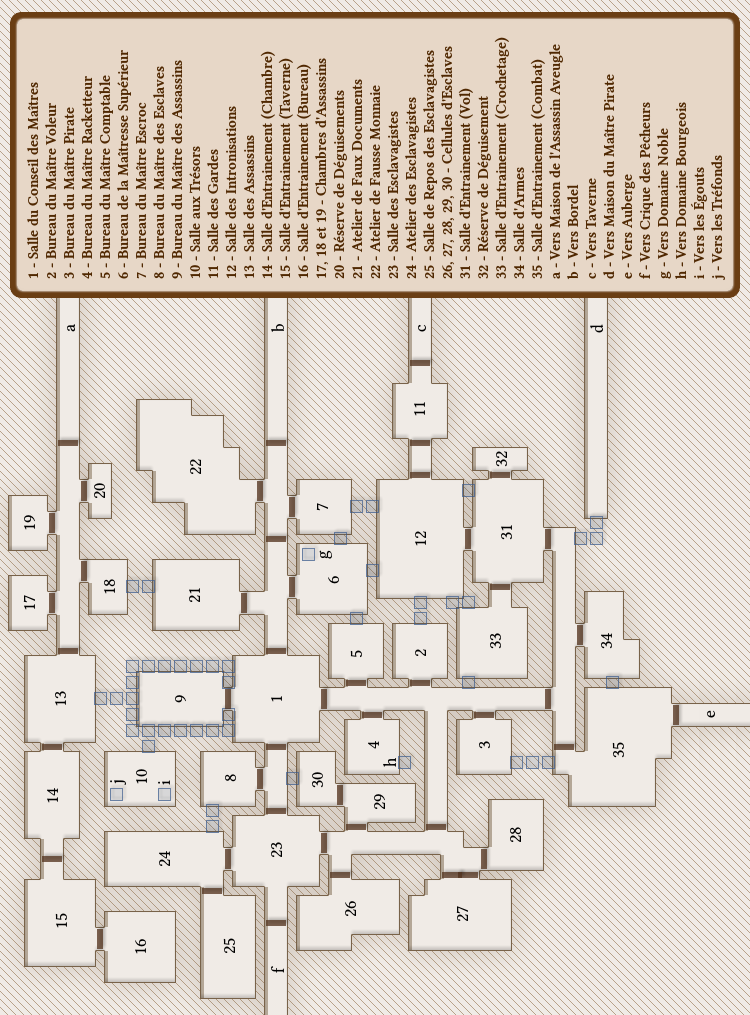
\includegraphics[width=16cm]{Maps/GuildeVoleurs.png}
\end{figure*}

\subsection{Les Différentes Branches}

\subsubsection{Les Groupes Locaux}

La ville de Sichua est en fait occupée en grande partie par des groupes
semi-indépendants ayant prété allégence à la guilde. Ceux-ci font appels 
à la guilde pour recevoir des renforts en cas de besoins ou de préparation 
d'un gros coup, mais doivent aussi s'aquitter d'une taxe auprès de celle-ci. Ils dépendent
d'un maître différent en fonction de leur localisation géographique:
l'ile de la source au maître assassin, le quartier des marchés au maître
comptable, le quartier du port sud au maître esclavagiste, le quartier 
bourgeois au maître escroc, le quartier pauvre du sud au maître racketteur,
le quartier du port nord au maître pirate, les quartiers nords au maître 
voleur et le quartier noble à la grande maîtresse. Cette dépendence hiérarchique 
n'empèche bien sur pas chaque groupe local de pratiquer n'importe lesquelles des huits
activités. Néanmoins, il est clair que ces groupes de petites frappes ne sont
jamais vraiment très puissant. 

Les groupes locaux ne couvrent néanmoins pas tout le territoire de la ville
et un certain nombre d'agents de la guilde dépendent directement d'un maître.
Ceux-ci sont en général les meilleurs agents des groupes locaux et sont recrutés
par la guilde pour s'occuper des affaires les plus lucratives directement. 
Les plus expérimentés obtenant finalement la direction d'un groupe local
si ils survivent suffisamment longtemps dans le milieu. Les chefs de groupe
locaux ont aussi un pouvoir important pour nominer un nouveau maître
lorsque l'ancien disparait. Ils décident alors de la promotion de l'un d'entre 
eux au rang de maître. Il est a noté qu'aucun groupe de malfrats n'est connu 
sur l'île de la source, le système de promotion du maître assassin échappe donc
à cette règle, mais reste un mystère pour le reste de la guilde.

%Liens vers groupe évoqué dans la quête ?


\subsubsection{Les Faussaires}

Dans le complexe de la guilde se trouvent deux ateliers important, l'un
accueillant de véritables artistes experts en conception de faux documents
et en imitations de signatures et l'autre est dédié à la fabrication de fausses 
monnaies. Le maître comptable est en charge de l'exploitation des ces deux
ateliers et de la diffusion de leurs produits. La fabrication de faux en
particulier est généralement utilisé pour des escroqueries de haut niveau
permettant souvent de voler de véritables fortunes.

Le maître comptable est un riche marchand qui tient un rôle clef pour
le blanchiment des entrées d'argent de la guilde dans son ensemble.
...

\subsubsection{Les Esclavagistes}

L'esclavagisme est interdit à Sichua, néanmoins il est possible d'y transferer
et d'y vendre vos esclaves si vous avez de bons contacts. Les esclavagistes 
utilisent une petite crique discrète dans le sud de Sichua pour transférer
les esclaves qui sont gardés directement dans les sous terrains de la guilde.
Ceux-ci seront exportés ensuite vers des îles loin au sud de Sichua, où la
pratique est légale. 

Le maître esclavagiste est un riche ...

\subsubsection{Les Escrocs}

Les escrocs de la guilde ont des activités multiples dans les jeux d'argents
généralement truqués. Ce groupe a aussi un rôle majeur dans le recel des 
marchandises volées par les autres branches de la guilde.

Le maître escroc est Meribald Dalloris (page \pageref{MeribaldDalloris}).

\subsubsection{Les Racketteurs}

Le principal rôle de ce groupe est de lever des "taxes" sur les marchands 
des quartiers les plus pauvres. Ils servent aussi de force de maintien de 
l'ordre à l'interieur de la guilde et peuvent être solicités pour remettre 
un groupe local sur la bonne voie. Enfin cette armée interne est parfois 
utilisée contre des concurents tentant de s'introduire dans la ville. 

\subsubsection{Les Pirates}

La piraterie dans les environs de Sichua a été éradiquée depuis longtemps,
néanmoins les navires marchands traversant l'océan des confins du nord au sud
crée une attraction irrésistible pour les loups de mer de tous horizons qui
guèttent leur proies potentiel au large du désert des ombres. Le grand dragon 
rouge Tarkin règne sur la région gardant les puissantes frégates de Sichua a
distance. Les pirates quand à eux prennent le risque... à moins qu'ils aient 
un accord avec le dragon et lui paye un droit de passage? 

Quoiqu'il en soit Sichua est le plus grand marché de la région et donc un lieu 
tout naturel pour écouler les marchandises accumulées. Le maître pirate est ainsi
plus un passeur qu'un véritable pirate et il sert de principalement de lien entre 
les pirates et le réseau de recelleurs de la guilde. La guilde de Sichua est aussi
le lieu où il peut vendre ses prisonniers comme esclave, optimisant ainsi ses 
voyages. 

Officiellement le maître pirate et ses hommes son équipage tout ce qu'il y a de 
plus respectable. Le maître pirate étant même un armateur important de la ville
avec de nombreuses connexions à la prévoté des marchands.


\subsubsection{Les Voleurs}

Les voleurs forment le c\oe{}ur de métier de la guilde et lui ont donné leur 
nom, mais cela fait bien longtemps qu'ils ont compris que parmis les diverses 
activitées clandestines pratiquée en ville se n'ést pas la plus rentable. Ils
ont reussit à tirer leur épingle du jeu en investissant les sous-terrains du
quartier noble et en dérobant il y a de nombreuses année le puissant artefact 
nain nommé "Keram Dek" ou "Pierre de Tranquilité". Celle-ci fut construite en 
des temps immémoriaux par les nains de la région pour empêcher les incursions
des races étrangères, en particulier en provenance des tréfonds.

Les voleurs de la guilde gardent un rôle important pour le recrutement au sein
de la guilde. Les plus doué des assassins et des faussaires de la guilde furent
ainsi tous recrutés enfant alors qu'ils pratiquaient de menus larçins sur un marché 
ou dans une taverne malfamée. Beaucoup de voleur se reconvertissent ainsi en
vieillissant pour mettre leur dextérité au services de travaux plus rentables...

Une petite partie des voleurs expérimentés rèstent néanmoins dans le groupe,
ils se chargent des cambriolages les plus complexes. C'est généralement le maître
voleur qui agit comme leader de cette équipe qui garde encore une grande fierté
d'être les descendants spirituels de ceux qui dérobèrent autrefois le Keram Dek. 

\subsubsection{Les Prostituées}

Alors que les prostituées furent longtemps exploitées par les racketteurs, elles 
ont finallement su trouver une place au sein de la guilde grâce à certaines d'entres
elles qui surent trouver des alliés au seins des autres factions de la guilde.
Celle-ci apprirent pour ce faire à exploiter les precieuses informations qui leur 
sont confiées par leur clients. A présent le rôle principal des prostituées dans la
guilde est de fournir les noms de riches personnages ayant des meurs particulièrement
aux racketteurs et escrocs, qui se chargent ensuite de faire fructifier ses 
informations. Les prostituées servent aussi souvent à isoler une proie pour un vol, 
voir même un assassinat. La rumeur dit même que certains assassins serait infiltré
parmis les prostitués. Point difficile à verifier tant le groupe des assassins de
la guilde est secret.

\subsubsection{Les Assassins}

Les assassins recrutent leurs hommes au sein de la guilde dans son ensemble,
recherchant les plus doués, mais aussi les plus taiseux et les moins alcoolisés.
Les rares sélectionnés restent généralement membre de leur anciens groupes mais
réduisent progressivement leurs activités alors qu'ils sont entrainés à l'art 
de tuer sans être vu... Il y a peut à dire à propos de ce groupe tant il est 
secret, à part qu'ils sont pret à prendre n'importe quel nom! Y compris celui
du duc lui même pourvu qu'on y mette le prix. 

\subsection{Rapports à l'Exterieurs}

Un accord secret avec les Alchimistes

Sert de source d'information à certains dirigeants

Siège au conseil des cinq

\subsection{Géographie de la Guilde}

{\bf Ajouter une table des pièges pour tirer au sort les effets des ouvertures.}
Verrouillé? Piégé? Type de piège? Désamorçage?

\paragraph{1. Salle du Conseil} Relativement grande salle voutée, elle comporte une
lourde table en bois entourée de chaises. Avec de lordes portes dans chaque mur.
Sous la table de la salle du conseil de la guilde des voleurs se trouve une stèle
de pierre gravée de runes naines émanant un pouvoir magique puissant. C'est un 
puissant artefact de dissimulation et de répulsion qui empêche tout ennemis de 
trouver le chemin menant au lieu qu'il protège. L'objet pèse une centaine de kilo,
mais si les aventuriers s'en emparent, ils permettent aux créatures des tréfonds
de remonter vers le complexe et déclenche une quête annexe pour sceller le túnel
après quelques semaines. Ils doivent ainsi descendre avec un nain expert mineurs 
qui indique ou ebouler le passage pour le bloquer définitivement. 

\paragraph{2. Bureau du Maître Voleur} Petite pièce avec un bureau en son centre.
La salle semble très banale mais comporte plusieurs secrets, à la 
fois dans le bureau et et dans certains murs. Le plus important d'entre eux étant
un passage vers un des balcons de la salle des intronisations. Les compartiments
secrets nécessite un jet d'investigation DC 20 pour être trouvé (faire 3 jets, 
bureau, coffres, passage), un jet DC 15 d'outils de voleurs pour être dévérouillé.
Si le joueur cherche, il découvre néanmoins que les passages sont piégés avec un 
jet de investigation DC 10, il peut aussi s'en appercevoir avec une perception 
passive de 15 ou plus. Dans le coffre se trouvent une amulette d'anti-détection,
des chaussons d'araignée et 3000 PO. Dans le bureau se trouve un anneau de saut et
un anneau d'action libre.

\paragraph{3. Bureau du Maître Pirate} Petite pièces aux murs couverts de cartes
maritimes, sur le bureau se trouve une maquète de navire. Le maître pirate 
disoposant d'un bureau plus luxeux dans sa propre demeurre, celui-ci est vide
de toute information et ne lui sert que pour rencontrer des membres de la 
guilde. Dans un tiroir de son bureau on peut trouver des yeux de lynx (page 
\pageref{}), un jet d'investigation DC 20 permet de trouver un compartiment 
dissimulés où se trouvent une cape de raie manta (page \pageref{}) et 1500 PO.
Découvrir le passage secret dans la salle nécessite un jet d'investigation 
DC 17 pour être trouvé.

\paragraph{4. Bureau du Maître Racketteur} Bureau assez dépouillé, le maître
racketteur étant illétré, il ne stoque aucun documents compromettants dans 
son bureau. Dans un tiroir non verrouillé mais piégé de son bureau on peut 
trouver quelques articles utiles à son travail: une flute de hantise (page \pageref{}), des 
gantelets de puissance d'ogre (page \pageref{}) et 800 PO. Un jet de perception DC 18 permet
de remarquer le mécanisme du piège un jet d'Éscamotage DC 18 pour le désamorcer. 
L'entrée secrète mêne à un escalier secret débouchant dans le domaine bourgeois
de la famille ... Le maître raquetteur a épouser la fille et héritière de la famille
dans des conditions louches, cela fait néanmoins de lui une personne respectable,
en façade tout du moins.

\paragraph{5. Bureau du Maître Comptable} Le petit bureau du maître comptable
à ses murs couvert de documents comptables. Ceux-ci sont nénmoins codé et ne 
permettent pas de découvrir qui travail avec qui précisément, Sr l'une des étagères
une lanterne ne semble pas payer de mine, mais un oeil avisé reconnaîtra une 
lanterne révélatrice (page \pageref{}). Dans le bureau
se trouvent quelques lettres possiblement compromettantes, si on 
arrive à passer la serrure et le piège de chaque tiroir. On y trouve aussi
des yeux grossissants (page \pageref{}) et 2000 PO.

\paragraph{6. Bureau de la Maîtresse Supérieur} Grand bureau aux murs couvert 
de velour, dans un coin un petit lavabo est aménagé et recouvert de parfums et
autres produits inconnu de la plus part des aventuriers.
Éventail enchanté, philtre d'amour x 3, potion de longévité, 500 PO

\paragraph{7. Bureau du Maître Éscroc}
Casque de Télépathie, poussière de disparition, 1200 PO

\paragraph{8. Bureau du Maître des Esclaves}
Chaines dimensionnelles x 2, sceptre tentacule, 250 PO

\paragraph{9. Bureau du Maître Assassin}
Tentures tout autour de la pièce derrière lesquelles on peut se dissimuler. 
Le maître assassin l'utilise et tente même de s'enfuir si les choses tournent 
mal.
Dague vicieuse, Cape de l'araignée, Cimeterre de rapidité, 2000 PO

\paragraph{10. Salle aux Trésors}
Gants de Combat (+1 et permet de ne faire aucun bruit lors des impacts pour
un combat a main nue, ajouter des propriété à débloquer), flêche mortelle 
pour humain, Manuel de coordination physique (pas encore utilisable à chaque 
séance un dé 20, sur un 20 le manuel est de nouveau utilisable!)
12500 PO (+ 7500 PO fausse perception passive DC 13)

\paragraph{11. }
\paragraph{12. }
\paragraph{13. }
\paragraph{14. }
\paragraph{15. }
\paragraph{16. }
\paragraph{17. }
Chambre d'Anderil, assassin d'hérinard. Une fiole de poison des enfers 
à demi vide sur le 
bureau posé sur un plan du temple de la justice permet de le déduire.
Possède une épée sanglante qui explique la marre de sang dans laquelle 
herinard fut retrouvé. Il discute avec un autre assassin du meurtre quand 
les joueurs arrivent. Ils peuvent entendre la conversation à travers la porte.


\paragraph{18. }
\paragraph{19. }
\paragraph{20. }
\paragraph{21. }


\paragraph{22. }
2500 PO de fausse monnaie.

\paragraph{23. }
\paragraph{24. }
Salle de travail, il y a un braséro et un fer de marquage. 

\paragraph{25. }
\paragraph{26. }
Divers esclaves Nain des Montagnes du sud.

\paragraph{27. }
Divers gnomes des roches du désert très au nord.

\paragraph{28. }
Un diable.

\paragraph{29. }
\paragraph{30. }
Le maître des esclaves original. Il est furieux car le maître assassin utilise 
sa marchandise pour invoquer des démons.

\paragraph{31. }
\paragraph{32. }
\paragraph{33. }
\paragraph{34. }
\paragraph{35. }

\paragraph{a. }
\paragraph{b. }
\paragraph{c. }
\paragraph{d. }
\paragraph{e. }
\paragraph{f. }
\paragraph{g. }
\paragraph{h. }
\paragraph{i. }
\paragraph{j. }





La tour phare de Sichua est visible à des dizaines de kilomètres à la ronde.
Elle est composée de différentes architectures au fur et à mesure de l'ascension.


C'est la résidence de l'archimage de la ville, l'école de magie et le 
phare qui guide les navires vers le port de Sichua. Ce batiment ancestral
a clairement été construit par magie et n'a probablement jamais dévoilé
tous ses secrets.

La tour semble faite d'obsidienne et s'élève a environ 120 mètres sur une 
colline qui en fait autant. Les etages de la base sont principalement 
remplis de l'administration de l'école, puis des résidences des étudiants, 
suivi des salles d'études. Arrivé au 20e commence la bibliothèque, un 
véritable labyrinthe qui couvre 5 étages. Ensuite les demeurre des 
professeurs occupent de vastes appartements et bénéficient d'une 
bibliothèque privée qui réunit les ouvrages interdits aux étudiants.
Les derniers étages sont réservé à l'archimage et ses assistants personnels
Une dizaine d'étage pour eux seuls pourrait sembler beaucoup, mais en 
réalité de nombreuses salles sont scellé et en cours d'études. Le mécanisme
d'allumage du phare est entretenu par les assistants de l'archimage et 
occupe les deux derniers etages.

Un secret bien gardé à Sichua est que dans les derniers étages
se trouvent quelques cellules pour les magiciens et autres créatures
qu'il ne serait pas sûr de garder dans la prison principale de Sichua.
L'éspérence de vie de ces personnes est fort limité, lorsqu'elles ont finit
par dire tout ce qu'elle savait ou en tout cas que l'Archimage le pense,
elle servent généralement a des expériences magiques jusqu'à ce que mort
s'en suive...

Les étudiants sont riches -> coût important de l'enseignement



\section{Temples de Sichua}

\subsection{Brève théogonie}
D'abord fut {\bf CHAOS}, célébré par les sans dieux, (non-)patron de la mer astrale. \\
Puis furent {\bf LUMIÈRE} et {\bf NUIT}, représentés par un dieu et une déesse, tous deux neutres, dont les religions sont oubliées. Ils formèrent les plans élémentaires et la magie.\\
Enfin vinrent les 9 dieux de l'archimonde: \\
- {\bf Dieu de la justice, ERIL (Céleste LB)} patron du plan de l'Elysée, grand temple en centre ville sur l'îlot. \\
- {\bf Dieu de la mort, OULTOR (Monstruosité-LN)} patron du plan de l'ombre, grand temple au cimetière du sud-ouest et chez les nains. \\
- {\bf Déesse des enfers, AZAZEL (Diable-LM)} patronne du plan des enfers, il est interdit mais les Hjelmaster ont un temple au sous-sol de leur demeurre. \\
- {\bf Déesse de l'agriculture, EWEA (Humanoïde-NB)} patronne du plan des champs infinis, grand temple sur la place du marché aux légumes, mausolées nombreux dans les faubourgs ouest et chez les nains. \\
- {\bf Dieu de la nature, SYLVANUS (Plante-N)} patron du plan materiel, temple à la source sur l'îlot. \\
- {\bf Déesse de la pourriture et de la décomposition, KEMILLE (Humanoïde-NM)} patronne du plan de la guerre, il est interdit mais quelques mausolées sont dans les égouts et dans les tribus d'orques, gobelins etc. \\
- {\bf Déesse des colporteurs et marchands, RILLA (Fée-CB)} patronne du plan féérique, temples nombreux sur la rive droite, principal au sein de la prévoté. \\
- {\bf Déesse de la mer et des tempètes, KIMA (Dragon-CN)} patronne du plan sauvage, grand temple sur un îlot devant la ville et des mausolées dans les ports. \\
- {\bf Dieu démon, THROKHRARTH (Démon-CM)} patron du plan des abysses, il est interdit mais il existe un cercle secret à sa botte. \\

\subsection{Temple de la Justice}

Dedié au dieu Eril, le temple de la justice trone en plein centre de la ville sur l'île de la Source.
On remarque immédiatement ce bâtiment massif à la façade couverte de marbre qui donne immédiatement
sur l'avenue du duc Erland. Plusieurs statues ornent la façade un dizaine de mêtres au dessus du sol,
celles-ci représentent les grands prêtres les plus illustres de l'histoire du temple. Celui-ci fut 
d'après la légende érigé aux débuts de la cités il y a environ 1400 ans, mais tout bon érudit vous
dira que c'est fort improbable. La cité était alors bien trop pauvre et un édifice aussi luxueu date très 
certainement du premier grand age d'or de la ville, il y a environ 1000 ans.

PNJ: Grand Prètre, Maître Paladin (Klermor d'Herinard), Le Grand Justice

\subsection{Temple de la Mort}

Au bord du grand cimetière du sud-ouest. Construction assez recente. Plusieurs petits mausolés annexes.

\subsection{Temple d'Azazel}

Temple secret dissimulé chez les Hjelmaster.

\subsection{Temple de l'Agriculture}

Au marché aux produits agricole, donne sur la place.

\subsection{Temple de la Source}

Dédié au dieu de la nature sur l'ile de la source dont il est l'origine du nom.

\subsection{Temple de la Pourriture}

Dieu interdit et essenciellement inconnu. Il en existe un temple caché, oublié de tous... pour le moment.

\subsection{Temple du Commerce}

Plusieurs temples en ville. Un grand temple forme une annexe au palais du prévot des marchands.

\subsection{Temple de la Mer}

Grand temple sur un ilot isolé devant la ville. Nombreux mausolés dans les zones portuaires

\subsection{Temple du Culte Démoniaque}

Enfoui sous la colline des nobles par un accès provenant d'un petit port du sud. Il est fréquenté par des pirates et des fous. Personne de sensé ne s'en approche sciemment.


\section{Monastère de la Sérénité}

Monastère à l'interieur du mur d'enceinte le plus récent. Il se trouve à 
l'extrème ouest de la ville au sommet d'une colline et est entouré de 
vignobles. Cette partie de la ville est peuplée par une communauté de
maraichers à majorité halfeline, humaine et demi-elfe.

Le monastère est principalement occupé par des moines de la voie de la
paume, quelques visiteurs pratiquant la voie des quattres éléments, mais
aucun de la voie de l'ombre. Cette dernière a mauvaise réputation depuis
quelques siècles car elle est utilisé par un groupe d'assassin. Les
membres du monastère gardent un oeil attentif sur tout moine de cette
voie qui pourrait se trouver en ville.

Le leader du monastère est appelé le guide, c'est un halfelin nommé 
Errimine Tarramane "calme mouvement" en céleste.

\begin{figure*}[tb!]
\center
\fbox{%
  \begin{minipage}[c]{.45\linewidth}
    \label{ErrimineTarramane}
    {\bfseries\LARGE\scshape Errimine Tarramane} \\
    Halfelin de taille S, neutre \\
    \noindent\rule{\textwidth}{1pt} \\
    {\bfseries Classe d'armure} 21 (porte des bracelets de défense) \\
    {\bfseries Points de vie} 110 (17d8+34) \\
    {\bfseries Vitesse} 15 m \\
    \noindent\rule{\textwidth}{1pt} \vskip 2pt
    \setlength{\tabcolsep}{4pt}
      {\footnotesize 
    \begin{tabular}{cccccc}
      \bf FOR & \bf DEX & \bf CON & \bf INT & \bf SAG & \bf CHA \\
       11 (0) & 20 (+5) & 15 (+2) & 13 (+1) & 22 (+6) &  15 (+2) \\
    \end{tabular} }
    \setlength{\tabcolsep}{6pt}
    \noindent\rule{\textwidth}{1pt} \\
    {\bfseries Jets de sauvegarde} For +6, Dex +11, Con +8, Int +7, Sag +12, Cha +8\\
    {\bfseries Immunités aux dégâts} poison\\
    {\bfseries Immunités aux conditions} charmé, empoisonné, effrayé\\
    {\bfseries Compétences} Acrobaties +11, Intuition +12, Perception +12, Persuasion +8, Survie +12 \\
    {\bfseries Sens} Perception passive 22 \\
    {\bfseries Langues}  Toutes \\
    {\bfseries Facteur de puissance} 11 (7200 XP) \\
    \noindent\rule{\textwidth}{1pt} \\
    {\bfseries Frappe étourdissante} Lorsque Errimine touche une autre créature lors d'une attaque au corps à corps, il peut effectuer une frappe étourdissante. La cible doit réussir un jet de sauvegarde de Constitution DD 20 sous peine d'être étourdie jusqu'à la fin du prochain tour d'Errimine. 
     \end{minipage}
  \hspace{4pt}
 \begin{minipage}[c]{.45\linewidth}
 \vspace{-10pt}
    \subsection*{Actions}
    {\bfseries Attaques multiples.} Errimine effectue quatre attaques au corps à corps : deux attaques avec ses mains et deux attaques avec ses pieds. \\
    {\bfseries Mains.} Attaque d'arme de corps à corps: +11 au toucher, allonge 1,50 m, une cible. Dégâts : 10 (1d10 + 5) dégâts tranchants. \\
    {\bfseries Pieds.} Attaque d'arme de corps à corps: +11 au toucher, allonge 1,50 m, une cible. Dégâts : 10 (1d10 + 5) dégâts contondants. \\
   \noindent\rule{\textwidth}{1pt} \\
Errimine est d'apparence très jeune et ne laisse rien paraitre de sa vie passé.
 \end{minipage}
}%
\end{figure*}


%TODO Bordel de la campagne

\chapter{Les Environs de Sichua}

\begin{figure*}[p]
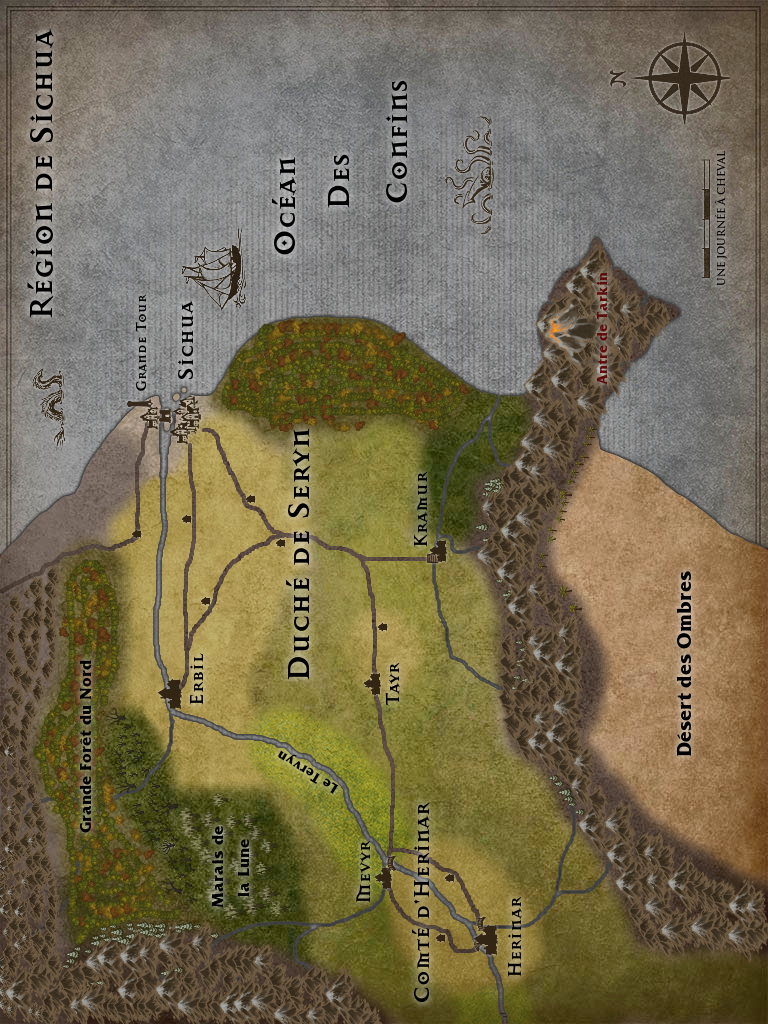
\includegraphics[width=17.5cm]{Maps/RegionL.jpg}
\end{figure*}

\section{Nobles et Territoires}

\section{Familles Nobles}

\subsection*{Harmar}
La famille d'Harmar est à la tête de la prison.

\section{Familles Bourgeoise}

\section{Autres Familles Diverses}



Décrire ici les Fiefs des nobles et répartission des populations.

Decoupage des territoires des tréfonds.

\section{Organisations}

\section{La Dergade}

\subsection*{L'organisation}

Réseau de contrebandier fournisseur de produits de contrebande en tout genre
en provenance des tréfonds et de certains plans peu fréquentables. Ils ont 
un monopole dans le duché de Sichua sur la pluspart des drogues disponibles. 
Ils disposent ainsi de champignons, spores, algues, mousses, venins et autre 
produits exotiques à l'origine douteuse possédant divers types de vertus 
euphorisante, halucinatoire, anesthésiante ou même calmante, mais très 
souvent aussi fortement addictive. On les soupçonne d'activité encore plus 
sombre telle que l'esclavagisme ou encore le commerce de produits alchimiques 
utilisé pour des invocations démonistes et autres rituels noirs. Moins connue
du grand publique est leur activité légale servant de couverture discrète aux
autres activités. En effet, un certain nombre de potions et sortilèges 
nécessitent des produits qui ne peuvent être trouvé que dans les tréfonds,
leur commerce est l'activité officielle des caravanes de la Dergade 
lorsqu'elles traversent les territoires.

Les accès aux tréfonds sont rares et le plus souvent secret, la Dergade 
utilise un passage à l'ouest des marais de la Lune connu d'eux seuls. Les
hommes de la Dergade connaissant le lieux sont tous sous l'effet d'un sort de
Mission leur interdisant de révéler l'emplacement du passage sous peine de
subir 5d10 dégâts psychiques. L'entrée vers les tréfonds se trouve dans les
ruines d'un ancien fort drow dont l'entrée discrète se trouve dans une grotte
au flan d'une colline perdue dans les steppes. La Dergade entretient une petite
troupe dans ce petit fort particulièrement discret. Néanmoins, ces collines
sont aussi sur le territoire d'un royaume d'orques particulièrement belliqueux.
Par chance, ou par design dirons les mieux renseignés, le roi des orques et
les grands prètres le conseillant sont accros aux spores de myconnides qu'ils
utilisent pour se ``connecter'' à leur divinité. Cet état de fait permet à la
Dergade de traverser les territoires orques en echange d'un petit droit de
passage...

Le comptoir de Kerlarflune dans les trefond est la destination des caravanes 
de la Dergade, il leur faut environ cinq jours pour le rejoindre depuis la 
surface. Ce comptoir tenu par des elfes noirs sert de point de rencontre 
entre les différentes communautés des trefonds, principalement pour le 
commerce et parfois pour des rencontres diplomatiques. Kerlarflune est tenu
par le Clan Deboer, un clan indépendant des grandes cités elfes noirs des 
tréfonds. Leur relative faiblesse par rapport aux grandes puissances les 
entourant fait d'eux un groupe insignifiant mais fort utile que toutes les
races des trefonds civilisées respectent, ou tout du moins tolèrent. Les 
membres de la Dergade sont suffisamment inelligent pour ne pas s'aventurer 
plus profondément dans les tréfonds.

\subsection*{Le Quartier Général}

Le QG de la Dergade est un hangar dans le quartier commerçant de Mevyr dans
le compté d'Herinar. Le hangar peut sembler modeste avec son exterieur 
discret et ses étales couvertent de produits que seul les érudits peuvent
reconnaitre, néanmoins il existe une arrière boutique... Celle ci n'est
par contre pas aisé à trouver, car quiconque ouvrant la porte arrière arrive
dans un bureau sombre et crasseux ou se trouve Karduc, l'homme lézard guerrier
officiellement propriétaire d lieu mais réellement seulement en charge de sa 
sécurité. La veritable arrière boutique est accéssible par la même porte,
du bureau vers le hangar, mais seulement si l'on prononce le mot de passe
"Tigre et Serpents" sans quoi la porte fonctionne de manière normale.  

L'arrière boutique accessible par cette porte secrète donne accès à un manoir
somptueux de Mordenkainen permanent. À l'interieur se trouve les reserves
de produits illégaux de la Dergade et surtout les appartements des deux
véritables dirigeants de l'organisation: Rénard et Serla, un Rakshasa et une
méduse. Ceux-ci fondent un couple fusionnel engagé dans le crime autant pour
s'amuser et l'adrénaline que pour l'argent. En cas de soucis, ils seront pret
à se sacrifier l'un pour l'autre, mais ne se préoccuperont pas le moins du 
monde pour un de leur subordonné. Si l'un deux est tué d'une manière ou 
d'une autre, le second mettra sa vie et la Dergade au seul service d'une 
future vengence. 


\subsection*{Idée d'Aventure}

Si les aventuriers obtiennent une réputation de mercenaires discrets, la
Dergade pourrait bien leur confier une mission. Aucune nouvelle n'a été
reçue de la dernière caravane envoyée à Kerlarflune, Rénard et Serla 
décident donc d'envoyer les aventuriers avec la caravane suivante pour 
assurer la sécurité du convois. Cette aventure peut aussi être initié 
par les joueurs eux même, si ils recherchent un accès aux tréfonds.

Le groupe se trouve attaqué par les orques sur le chemin qui semblent 
determinés contre toute intrusion dans leur 
territoire. Ils trouveront ensuite à l'entree des trefonds les corps des 
gardiens de la Dergade, ceux-ci sont eparpillés dans plusieurs pièces et 
portent tous des blessures profondes infligé par une créature certainement 
massive et puissante. Ce sont en fait des ombres des roches qui ont fuit
et que le groupe peut chasser en surface, maintenant ou plus tard. 

Une fois arrivé à Kerfarflune, le groupe trouve un comptoire en partie détruit 
et dont il rèste que quelques groupes cloîtré dans des grottes. La caravane
peut y vendre sa marchandise (essenciellement de la nourriture de la surface
(miel, épices, fromages, vins etc.) à prix d'or, les survivants étant pret 
à payer très chère pour quelques fournitures. Par contre, ceux-ci ne dispose 
pas de grand chose à part de l'or, en particulier très peu de produits 
stupefiant. Il retrouve sur place un ou deux membres de la precédente 
caravane qui leur explique que des monstres défèrlent regulièrement depuis
pusieurs semaines.

Si les aventuriers explorent plus en avant, ils découvriront à l'origine 
de ces créatures, le nid d'un groupe de dévoreurs mentaux. Ceux-ci semblent 
avoir été décimés et leur esclaves se sont echappé dans les tréfonds créant 
tout ces troubles. Une enquête approfondie indiquera que le nid à eté détruit
par un ver pourpre, un expert ou un survivant permettra aux aventuriers de
comprendra que l'une des larves de dévoreur s'est échappé de leur couveuse.
Elle est finalement revenu après avoir grandi dans des proportions démesuré
et a détruit le nid de sa naissance. Il est bien sûr possible de se lancer 
à la poursuite de la bête, aux risques et périls des aventuriers. Néanmoins 
la découverte precédente indique clairement que les attaques devraient 
rapidement se rarefier, les dévoreurs n'ayant eu qu'un nombre limité 
d'esclaves à l'origine. 



\section{Lieux}

%L'antre de Tarkin

%Les montagnes géantes

%Les collines des gnolls

\part{La Campagne}
% Ajout d'une intro


\section{Introduction}

La campagne troubles à Sichua permet d'exploité une grande partie des lieux présentés dans la partie 
précédente. Elle est composée de nombreuses séquences indépendentes qui peuvent être jouées indépendament
ou intégrées dans une campagne différente. Le nombre d'aventures proposées dans la campagne est 
volontairement important. Les joueurs n'en effectuent qu'une fraction et peuvent
se dirgier vers les différentes parties de la campagne librement. 

Lors de la campagne les menaces se multiplient en ville et celles qui ne sont pas circoncites par les 
joueurs prennent de l'ampleur et forment la base pour des menaces futures. Au fur et à mesure de la campagne
les joueurs en apprennent plus sur l'histoire de Sichua et la menace qui pèse sur la ville.

\section{Plan de Campagne}

{\bfseries Troubles à Sichua} \\
{\bf 1} Découverte d'un des adversaires secondaires {\it 1-3} \\
{\bf 2} Les PJs s'en occupent eux même et tuent l'adversaire {\it 4-5} \\

{\bf Chaos à Sichua} \\
{\bf 3} Leur principal commenditaire est assassiné en réponse
  Les PJs doivent remonter au démoniste ou nécromant selon qui a survécu.
  Tentative d'assassinat contre les PJs avant d'arriver au but {\it 6-7}. \\

{\bf Le Cerveau se Révèle} \\
{\bf 4} Avec les papiers du survivant les PJs trouve le donjon des voleurs/assassins. 
        Les PJs infiltrent le donjon de la guilde des voleurs et combattent le maître assassin {\it 8}.
{\bf 5} Prise d'assaut de la maison van Hjelmaster pour achever le maitre qui est un vampire. {\it 9}.
  Enquete dans le complexe des voleurs, la ville surplombe un important réseau d'outre terre abandonné par tous. \\

{\bf Une Nouvelle Menace} \\
{\bf 7} Créatures puissantes dans les environs -> proviennent d'outre terre {\it 10}.
  Il va falloir descendre s'occuper de ce qui remue en dessous... \\
{\bf 8} Descente dans l'outre terre et découvrerte du monde d'en dessous.
  Nombreuses rumeurs circulent sur la liche flageleuse mentale. {\it 11}
  Les joueurs tuent un nombre important de monstruosités, mais la liche n'est pas dans son domaine {\it 12}.
  Enquête, quel est le plan de la liche? Compréhension et remonté en urgence \\
  La liche compte ouvrir un portail vers les abysses et attirer de puissants princes démons sur Sichua. 
  Pendant ce temps la liche compte se rendre dans les abysses et s'y tailler un royaume pendant que les plus 
  puissants démons sont affaiblis par leur guerre dans le plan materiel. \\

{\bf Un nouveau monde} \\
{\bf 9} Interrompre l'incantation d'un portail par la liche {\it 13}. \\
{\bf 10} En cas de succès aller la dénicher dans la grande tour des mages où elle s'est réfugiée {\it 14}. \\
{\bf 10 bis} En cas d'echec, vaincre les démons qui ravagent la ville (la liche est partie en enfer) {\it 14}. \\

{\bf En enfer} \\
{\bf 11} Pour en finir une bonne fois pour toute, les joueurs vont devoir aller en enfer finir le boulot. 
Soit pour se débarrasser du prince démon qui veut absolument prendre la fontaine de vie. \\
{\bf 11 bis} Soit pour aller tuer la liche dans les abysses. {\it 15} \\

{\bf Sichua en ruines} \\
{\bf 12} A leur retour les joueurs trouvent Sichua en ruines, les géants sont en train de 
mettre à sac la ville et on dit que c'est un dragon qui les mène! Les joueurs libèrent la ville. {\it 16}
{\bf 13} Le dragon débarque et combat les joueurs. {\it 17}

\chapter{Troubles à Sichua}

\section{Introduction}

Missions Part-branche-numbranche. Ajouter un guide pour naviguer entre les missions.

Joueurs:
\begin{itemize}
  \item {\bf Ghech} sorcier drakeïde (Mikael)
  \item {\bf Myrdim} barde demi-elfe (Kévin)
  \item {\bf Seyonne} moine demi-elfe (Julien)
  \item \sout{{\bf Mialee} ranger haute elfe (Cyrielle)}
  \item {\bf Thia} druide haute elfe (Cyrielle)
\end{itemize}

Ghech est lié avec un grand-ancien par un pacte de chaine. Son familier est un 
monodron. Le grand ancien est à la recherches de connaissances pour une raison
inconnue.

Myrdim est un peu kleptomane, ce qui lui attire des ennuis régulièrement.

Seyonne a appris son art auprès de démonistes qui l'avaient enlevés

Mialee accueille un groupe d'orphelin dans leur petite maison délabrée. Elle
est malheureusement décédée lors d'une rixe dans les faubourgs nord.

Thia, la s\oe{}r de Milee est une druide du temple de la nature en centre ville.

\section{Troubles à Sichua}

Le groupe de joueur a la liberté de démarrer ses recherches de différentes manières en fonction
du passé des personnages et de leur motivations. Ensuite, la manière dont leurs aventures se déroulent
peuvent changer du tout au tout leur parcours, si ils s'adressent au temple ceux-ci peuvent les rediriger 
vers le cultistes. Une rencontre aléatoire peut les faire se rediriger vers la recherche du nécromancien 
ou encore la recherche d'argent peut les amener à travailler avec la guilde des alchimistes. Dans tout
les cas, cette première partie de la campagne se termine lorsqe les joueurs défont l'un de ces trois
adversaires.

\subsection*{1-1-1 Les rats géants}

Depuis quelques temps des rats géants sont apparu en ville. 
Plusieurs chambellans de quartiers touché offrent une PO par carcasse.
Deux exemples de chambellans: Familan un marchand de pots en cuivres et 
casseroles, c'est un vieux monsieur avec de l'embonpoint et une grosse 
moustache blanche. Il peut orienter les PJs vers la quête.
Orond est lui chambellan au c\oe{}ur des quartiers attaqué par les rats,
c'est un maréchal férand plutôt jeune avec une barbe noire raisonnablement
taillé. Il est musclé et généralement transpirant dans sa boutique sur chauffé.
Devant chez lui s trouve un tas de cadavre de rats.

Nos jeunes aventuriers peuvent tenter une incursion dans les égouts pour trouver un grand nombre de rats.
N'importe quel habitant sait que les égouts sont un endroit dangereux pour une personne seule, mais pour 
un groupe, normalement il n'y a pas de problème.

Etape 1: Rassembler des informations et de l'équipement (torches et barre à mine sont utile)

Etape 2: Se rendre de nuit dans le quatier le plus infesté. Il y a quelques autres groupes qui cherchent
des rats. Ils sont formé 1d4+2 bandits MM343. Les PJs et un groupe découvrent 5 rats géants MM327, le 
meilleur jet de survie mène la traque. S'en suit une dispute sur qui doit récupérer les corps pour la 
prime. Tout est possible, jets contesté DC fixe en fonction de la force de l'argument. Si ils tuent les
autres aventuriers -> Mission échapper à la garde.

Étape 3: La victoire pousse le groupe à descendre dans les égouts. Descriptions égouts, odeur infame,
champignons géants dans tous les coins (DC15 nature pour les reconnaitre, jet de sauvegarde sagesse DC15 
pour ne pas s'evanouir si on y touche). On entend en permanence les couinements de rats (non géant) 
provenant de toute part, on les aperoient aussi à la limite de la lumière de la torche. Les aventuriers 
poursuivent quelques rats géants 
isolés (combats non joués). Ils en attrapent un toute les 10 minutes environ, après 1d4 rats capturés, 
jet de survie DC12 pour sentir qu'ils approchent un "nid" affrontent 5 rats géants MM327 apres deux 
tours 2 rats géants supplémentaires
arrivent par derrière. Certains rats semblent a moitié pourris comme si ils étaient dejà mort...

Étape 4: Sur le retour, l'aire semble lourd et le silence est complet dans l'égout. Certains des corps 
de rats aux ceintures se mettent à fremir et bouger... Sans barre à mine
jet DC 12 survie pour retrouver leur chemin. Sinon jet DC15 force pour ouvrir une porte. En cas d'échecs
ou de non fuite, deux squellettes apparissent MM272. A la fin du combat 1d6 corps de rats perdu semblent 
avoir fuient. Deuxieme tentative de sortie réussie sinon arrivent dans un couloir ou se trouvent une dizaine
de squelettes. Fuite oblegatoire.

A la sortie de l'égout l'équipe gagne un 300 xp et peut aller faire un rapport au chambellan. Il est
séptique et renvoie les PJ vers le temple de la justice sur l'affaire des morts vivants.

\subsection*{1-1-2 Un nécromant en ville}

Au temple on leur propose: Rencontre Temple démonistes (Mission 1-3-1) ou de ramener une preuve et une 
localisation précise. Les paladins préviennent néanmoins les PJs qu'un nécromant capable de lever une
armée de squelètes est certainement bien trop dangereux et ils doivent se contenter d'observer si il
y a réellement un nécromancien dans les égoûts.

Klermor d'Herinard -> Paladin au temple de la justice (Eril)

Etape 1: Enquete dans les sous sols 
 -> Quelques rats (bcp de rats morts)
 -> Jet de survie DC15, en cas d'echecs tombe dans une embuscade de champignons -> 5 violet fungus MM 138
 -> Trouve une "habitation" le necromant a fuit
 -> Les PJs tombent dans une embuscade -> 2 spectres mineurs MM 279 dont un poltergeist -> HP 18 domages 2d6 +3 pour toucher.
 -> Autel de pierre gravé de symboles étranges

Etape 2: Retour au temple
 -> C'est un signe d'un diable. Le nécromant a fait un pacte avec les enfers -> Azazel - Prince des enfers DC20 religion
 -> Envoie les PJs surveiller le cimetière du sud pendant la nuit en attendant
 -> Troisième nuit -> rencontre morts vivants -> rats nombreux si rien n'a été fait avec le tas de chez Orond -> 8 Giant zombie rats MM 327 -> fortitude du mort vivant MM316
% Statut de mon groupe actuel
 -> Rencontre le gardien du cimetière Paire en fait le nécromancien déguisé -> leur indique l'origine des troubles, un mosollé -> 2 ghouls MM148
 -> Découvrent un campement précaire

Etape 3: Rapport au temple
 -> Trop occupé avec un culte démoniaque qui prend de l'ampleur
 -> Conseil aux PJs de garder le cimetière contre le nécromancien
 -> Embuscade par des golems de bois qui remplaçaient des bancs
 -> Attaque par deux espions MM349 de nuit chez eux


\subsection*{1-1-3 En guerre contre la mort}

Etape 1: Surveillance de divers cimetières
 -> Finissent par attraper un groupe de pilleurs de tombe COMBAT
 -> Ils revendent les corps à la tour des mages, mais il est hors de question de témoigner -> ils ont peur

Etape 2: Un adversaire identifié
 -> Arrivent a découvrir les allés et venues suspicieuses du nécromant
 -> Lorsqu'il est attaqué il fuit avec porte dimensionnel et laisse les Pjs dans une embuscade COMBAT
 -> Renseignement sur son identité -> il est trop important pour être arreté sans preuves en béton

Etape 3: Aller chercher l'ennemi dans sa tanière
 -> Infiltration de la tour ou de la demeurre et COMBAT nécessaire
 -> Surveillance de la tour
 -> Golems de bois dans son salon
 -> Le dernier combat du nécromant


\subsection*{1-2-1 Sur la piste du fungus}

Un alchimiste du nom de Ferrangus emploie les aventuriers pour aller chercher des champignons dans les
égouts. La mission est identique à 1-1-1, cueillir les champignons nécessite un jet sleight of hand DC15
si les PJs savent qu'il est dangereux. Sinon échec automatique. 1d6 dégats psy à cause des spores.

Peut rediriger vers la recherche des mort-vivants 

\subsection*{1-2-2 A la chasse}

TROUVER CREATURES a chasser qui soit logiquement à la base de la création de golems. Doit comporter
un dilemme moral moyen de plus en plus fort

\subsection*{1-2-3 Une sombre affaire}

Infiltrer les combats clandestin de rue pour enlever des gladiateurs. Ceux ci servent à fabriquer
des golems de chair. Dilemme moral majeur. Les PJ comprennent qu'ils travaillent pour un criminel
dangereux!

\subsection*{1-3-1 Un culte turbulent}

Depuis quelques jours, les membres du temple du dieu de la justice (un groupe de clercs et paladins) 
suspectent la présence de démonistes. Malheureusement c'est hors de la ville dans un faubourg 
et donc sous la juridiction du duc qui n'est pas du tout interessé par ces histoires de religions.
Les paladins ne peuvent intervenir directement, il souhaitent que les PJs aillent jeter un oeil.

Étape 1: Le faubourg est pauvre et principalement habité par des ouvriers agricoles. Les aventuriers
s'y rendent, si ils questionnent à propos d'une secte, ils sont attaqués par 3 acolytes MM342. Si ils
trainent suffisamment dans le quartier avec un look assez pourri, ils se font alpaguer pour joindre le 
culte à minuit. Sinon ils doivent faire parler un cultiste.
-> Derrière l'auberge du fer à cheval se reunissent les membres du culte

Étape 2: Surprendre les cultistes. Les PJs peuvent assister aux culte en tant que croyant ou en éspions.
En tant que croyant, on leur demande de boire une coupe de sang "humain" (en fait du sang de cochon).
Les cultistes ne semblent pas très dangereux. Par contre, si ils sont pris à éspionner ils se font 
poursuivre par un groupe de paysans armés de gourdins MM345.

Étape 3: Les PJs font leur rapport au culte. Ils se font jeter si ils ont tués des civils, les paladins ne 
les étrippent pas simplement pour ne pas être impliqué. Sinon, les paladins proposent de payer plus pour 
que les PJs continuent à enquêter sur le leader du culte.

Étape 4: Les PJs peuvent essayer de coincer Bardan le gourou du culte (Fanatique MM345). Il ne parlera
sous aucun pretexte. Les PJs s'aperoivent que c'est un vrai clerc d'un dieu démoniaque. Il porte sur lui 
une amulette (CA+1). Le porteur commence à faire des cauchemars.

\subsection*{1-3-2 Un véritable culte démoniaque}

Le porteur de l'amulette se fait aborder dans la rue par un cultiste. Si il sont consulté les paladins
proposent aux joueurs de s'infiltrer dans le culte au plus haut niveau. Le groupe se fait enroler. 
Les premières missions sont raisonnable et consiste a trouver un lieu de culte (nettoyage de quelques
fungis et morts vivants dans les egouts). Assez vite les cérémonies deviennent macabres, des hommes se 
scarifient au début, puis se sont des étrangers qui sont torturés. Un jour un jeune paladin a le coeur 
arraché, l'un des pj doit aider a tenir la victime. On demande au PJ d'enlever d'autres paladins ou
clercs et on leur propose de se scarifier. La seule question est quand arreteront-ils les frais. Vers le 
milieu de l'initiation, ils identifient le véritable leader du culte.

\subsection*{1-3-3 Détruire le culte}

Le culte commence a invoquer des démons la déstruction (ou l'alliance totale?) devient nécessaire.

Les Paladins peuvent aider, la principale difficulté est de coincé les chefs du culte et en particulier
le sorcier. Il faut aussi affronter des invocations d'autant plus puissante que les PJs ont tardé à changer
de piste. 


%TODO Ajouter des indices qu'il y a un maitre derrière tout ça




\chapter{Chaos à Sichua}
\section{La Mort aux Trousses}

\subsection*{Introduction}

Suite à la révélation de la connexion entre les différents troubles dans a ville et
la découverte de l'un des membres éminent du culte d'Azazel, le culte d'Azazel décide 
de répondre avec force. Ce chapitre de l'aventure commence par l'assassinat du 
principal allié des joueurs et par l'augmentation significative des troubles en ville.

\subsubsection*{Choisir sa voie}

Le groupe est introduit auprès du conseil des cinq. Ceux ci leur demande de 
résumer leurs découvertes. Les joueurs choisissent un patron parmis les cinq.

Selon le niveau de débrouillardise des joueurs, il faut les pousser plus ou moins.

Il y a trois voies possibles, l'infiltration de la guilde des voleurs, l'infiltration
démonistes (si ils n'ont pas été détruit), l'infiltration des chasseurs de monstres,
les troubles nécromantiques.

\subsection*{L'invasion de morts vivants}

\subsection*{Le Culte Démoniste}

\subsubsection*{Infiltration}
Si ils ne l'ont pas déjà, leur patron fournit l'amulette d'Azazel

\begin{figure}[htb!]
\center
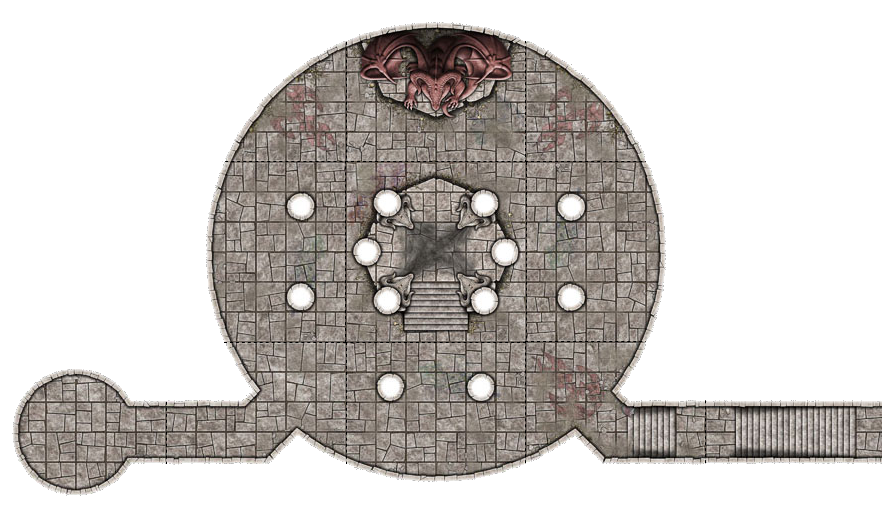
\includegraphics[width=7cm]{Maps/Temple.png}
\end{figure}

Le groupe se rend dans les quartiers où se trouvent le plus de démonistes. 
Alors qu'ils mènent leur enquête, ils sont guidé vers une auberge où se 
trouverait des cultistes. Alors que les joueurs sont dans l'auberge des sons 
étranges résonne dans le bâtiment. Le groupe est alors attaqué par un Vrock
(page \pageref{Vrock}). Lorsqu'ils trouvent le lieu d'origine de la bête, ils trouvent un 
pentacle de sang au sol et quelques cultistes qui se sont apparement saigné 
à mort pour l'invocation.

L'intérogatoire d'un survivant révèle que chaque meneur rassemble un petit 
cercle de fidèles et les dirigeants se regroupe dans une instance plus 
importante. Le groupe devra les infiltrer pour découvrir qui dirige réellement
le culte.

Dans le sous sol d'une auberge (potentielle aquisition du groupe)
Prendre la place d'un meneur -> combattre un Diable à chaines.
Meneur ancien tenancier "???"
Ses patrons "Godrik" "Keltar" "Ernoc"

Description de l'auberge, grande salle ronde au sous sol. A l'étage, les 
chambres sont surtout louée à des cultistes. Chambre principale occupée par le leader.

Participation a une première réunion.
Le groupe est demandeur d'exaction. Conundrum moral. Peuvent executer un comdamné à mort ou autre.
Proposition de duel (un contre un) en fin de réunion (challenge majeur). Les joueurs peuvent attendre une meilleure
occasion hors réunion (il faut ensuite convaincre le culte que la prise de 
pouvoir est légitime: autre combat) ou préparer la rencontre de fin de réunion avec des potions, buffs divers lors de la réunion suivante.


Appel auprès du grand chef. Réunion dans le cimetière du nord. Demande de rassembler des os d'humanoides 
pour une invocation. Ceux qui en ramèneront le plus participeront à l'invocation et gagneront les faveurs de Azazel.
Il sacrifie une jeune femme en fin de réunion sur l'autel.  Occasion en or de l'attrapé isolé.

Options: piller des catacombes ou s'attaquer à une tribu de gobelinoides en marge de la ville et trouver leur cimetière. Il faudra en ramener une carriole!

\subsubsection*{Piller les anciennes catacombes}

Les anciennes catacombes sont vieille de plusieurs siècles, peut être millénaires, elles datent d'une époque où 
les nécromanciens étaient trop nombreux et où il n'était pas raisonnable de conserver des corps 
en grande quantité dans la ville. Les catacombes se trovent à deux jours de marche environ au sud 
de Sichua, le voyage traverse des territoires vallonés et agricoles. Les catacombes se trouvent à
l'auré d'une grande forêt encore sauvage. Les rumeurs sont nombreuses et suffisament effrayante pour
avoir stoppé la progression de la civilisation dans cette direction. Si les joueurs mènent une enquête
dans les alentours sur ces rumeurs, un jet DC 12 en investigation leur permet de s'appercevoir qu'entre
les multiples histoires de fantômes, spèctres, goules et autre morts-vivants, il est aussi souvent 
question d'une sorcière faucheuse d'âmes.

Le patron des aventurier leur fournit une petit cariole avec sa mule et trois barils à remplir 
d'ossements. Un guide connaissant la région les accompagne aussi, malheureusement, celui-ci est
incapable de combattre efficacement (statistiques page \pageref{Eclaireur}). Lorsque le groupe
arrive sur place ils découvrent un ancien temple en grande partie détruit en l'honneur du dieu 
de la mort. Le temple est envahi par la végétation et la forêt alentour est particulièrement
épaisse et impénétrable, il semble impossible d'aller plus loin avec la carriole. Dans les 
décombres du temple derrière l'autel se trouve une arche de pierre avec des runes servant 
d'entrée à un tunnel, c'est très certainement l'entrée des catacombes. Un jet de religion
DC 15 permet d'interpreter ces runes magiques, celles-ci permettent de bloquer le passage
de tout mort-vivant dans un sens ou dans l'autre.

Affrontement de morts vivants qui semblent particulièrement excités.

Fantome en entrant

Arrivé aux catacombes les os semblent s'activer, 6 squeletes et minotaure.
Dans la salle une fouille rapide permet de trouver une lantern of revealing 
sur des ossements plus récents. Probablement ceux d'un pilleur de tombe, la 
lanterne parait intact ce qui attire l'oeil, l'objet semble magique.

Tombe sur une hag qui se considère propriétaire des ossements et compte bien tirer quelque chose des joueurs.
Pendant que ceux-ci visitent la crypte elle tue et remplace le guide des joueurs. Si les joueurs ne voient pas le coup
venir, elle hante l'un d'eux duran la nuit. Elle fera le nécessaire pour tuer un joueur et voler son âme avant de s'enfuir.

Au cas ou l'équipe arrive a tuer la hag, sur son corps ils trouvent plusieurs objets magiques, un 
anneau de barrière mentale (page \pageref{AnneauBarriereMentale})
et une flasque de fer (page \pageref{FlasqueFer}). Elle dispose aussi sur elle d'une statuette en
or, un jet religion DC 15 permet de connaitre une version primitive de Eril dieu de la justice.
Si les joueurs le ramène au temple de la justice, il l'échange contre le marteau de tonnerre.
Cette dernière si elle est activée 
révèle une jeune femme appeuré qui déclare
s'appeler Sélia et avoir été enlevé, c'était il y a fort longtemps et elle ne se souvient de rien
de sa vie passé. En fait c'est une succube, Joaline, (page \pageref{Succube}) qui 
tentera d'user de ses charmes sur l'un des joueurs
masculin de préférence. Si elle est découverte elle tentera de fuir. Elle porte un anneau de 
régeneration (page \pageref{AnneauRegeneration}).

Une fouille approfondie des catacombes durant une journée se fait sans rencontre supplémentaire
à l'exceptions de quelques squelettes (combats non joués). Un jet d'investigation DC 15 permet
de trouver un objet d'intérêt. Dans la tombe d'un barde se trouve une mandoline magique
(Canaith Mandolin, Instrument de Barde, pas sur AideDD. Faire un objet concient ou l'esprit d'un
ancien barde est piégé).

Passage niveau 6.

\subsubsection*{Chasse aux Gobelins}

Affrontement d'une troupe de chasseurs isolés

Combat pour leur ancien lieux de culte 

Poursuite pour échapper

\subsubsection*{Démanteler le culte démoniste}

Au retour en ville le groupe trouve une ville en émois et un combat éclate dès 
les faubourgs avec des diables: trois chiens des enfers 
(page \pageref{ChienEnfers}). Après ce combat, les joueurs apprennent
que la garde a du mal a maintenir la paix simplement dans les murs. Les faubourgs 
sont abandonnés aux diables. Lors de la prochaine réunion, il va falloir suivre
quelques leader cultistes et faire du ménage discrètement en attendant le gros 
évenement. 

En attendant l'appel les joueurs peuvent tenter de trouver l'un des cultes et tuer son 
leader. Ils peuvent ainsi s'attaquer à la ferme de la réunion qui est en fait le centre
d'un culte ou enqueter en ville. Quoiqu'il en soit, leur adversaire est un diable à 
chaine accompagné d'un chien des enfers (pages \pageref{DiableChaine} et \pageref{ChienEnfers}).

A la réunion suivante les cultistes se regroupent dans les faubourgs dans un petit champ
derrière une ferme. Le leader cultiste distribue des parchemins d'invocations de chiens 
des enfers et conseille à chacun d'invoquer massivement dans les jours qui viennent.
Le parchemin nécessite le sacrifice de trois personnes pour s'activer. En matière 
d'ossements, les membres du groupe gagnent la petite compétition. Le leader
les felicite de leur intelligence d'aller chercher l'exterieur de la ville. Il 
convoquera le guide du groupe lorsque tout sera pret pour l'invocation. (en cas d'échec
à la mission precedente, les joueurs doivent suivre le vaincoeur et prendre
sa place dans la plus grande discrétion).

Les membres du culte des joueurs demandent une invocation dans leur groupe, car il y
en a eu plusieurs pas loin. Certains membres quittent le groupe pour rejoindre
des voisins. Si les joueurs ne font pas quelque chose, ils reviennent pour les
abattres (trois Cult fanatics, un chien des enfers et un gladiateur 
(gants de force d'ogre) . Les joueurs 
peuvent s'attaquer aux voisins (meme troupe a vaincre), mais attention, il va falloir 
être discret et ne pas se griller dans le culte d'Azazel. Si l'invocation est 
effectuée par l'un des joueurs, sont prochain niveau est automatiquement un 
multiclassage sorcier (si il ne l'a pas déjà) avec Azazel comme patron. (Ce niveau 
pourra être annulé et repris comme un niveau du choix du joueur à la fin du chapitre).

L'appel vient finalement, rendez vous dans des caves sous les collines du sud.
Un véritable labyrinte où sont enmenés les ossements. Les joueurs sont attaqués
à la sortie de leur base par un concurrent mécontent d'avoir été doublé, c'est
un cambion, accompagné d'un chien des enfers (pages \pageref{Cambion} et \pageref{ChienEnfers}).
Ils peuvent les avoir tuer si ils ont suivi l'un des chefs cultistes lors de la 
réunion. Le cambion porte une armure d'écaille de mithril et 550 po. Nom: Aturik.
(Ajouter des trucs dans le hangar).

\subsection*{L'invocation}

Les joueurs sont convoqué dans une auberge du sud au pied des falaises 
sous la colline ou habite les familles fortunées. La cave de l'auberge s'étend 
sous la colline et les joueurs y trouvent un grand temple qui a été visiblement 
réamenaagé pour le culte d'Azazel. Seul le leader du culte est néanmoins invité à
l'interieur. Le temple est installée dans une grande caverne avec au fond une 
énorme statue d'Azazel. Au centre se trouve un pentacle géant où sont accumulés
tous les ossements rassemblés précédemment. Deux golems de chaire sont aussi
présent dans le temple avec Krassius Eldark qui indique à son invité que lui 
et les golems sont là pour sécurisé les lieux durant l'invocation. Si son rituel
devait être interrompu, le portail deviendrait instable et risquerait fortement 
de tout absorber!

Le rituel prend 1 minute (10 tours). Au premier tour apparaissent 3 quasit,
au deuxième tour deux shadow demons, au troisième tour un chasme et au cinquieme
tour un Vrock (page \pageref{Vrock}). Ces démons et diables attaquent les créatures
les plus proche d'eux de manière aléatoire. Les golems font écran pour protéger
Krassius. Au dixième tour un diable cornu nommé
Andear (page \pageref{DiableCornu}) apparait, celui ci idenifie immédiatement 
les aventuriers comme des traitres et agit de concert avec Krassius. Le seul moyen
de mettre fin au rituel avant qu'il soit complèter est de tuer Krassius. Celui-ci
n'agit pas durant les dix tours de l'invocation et reste concentré quoiqu'il arrive.
À la fin du rituel, ses pouvoirs magiques sont épuise et il se contente de s'éloigner
du portail puis d'utiliser ses cantrips dans le combat.

%TODO ajouter les démons et les liens correspondant.

Dans le cas où le rituel est annulé ou terminé, le portail se referme.
La fermeture du portail prend 3 tours causant des dégâts comme il suit. 
Durant ces trois tours les créatures à
moins de 6 mètres du pentacle doivent faire un jet de sauvegarde en force DC15, 
ils subissent 8d6 dommages de force et leur vitesse est divisée par deux jusqu'à 
la fin de leur prochain tour en cas d'échec ou subissent simplement la moitié des dégâts 
en cas de succès. Les objets non portés et les corps inanimés à porté du portail
sont aspirés et transportés dans les neufs enfers (localisation exact aléatoire).

Les personnages réstés à l'extérieur doivent passer quelques cultistes mineurs 
pour arriver au temple en toute discrétion. Il est important que les joueurs
indique quel trigger les fera intervenir ou entrer dans l'auberge pour éviter
une influence des évènements qu'ils ne sont pas sensé connaître. Un jet 
d'investigation DC 15 sur les alentours de l'auberge, leur permet de comprendre 
qu'il y a possiblement une partie troglodyte dans l'auberge.


En fin de combat, le maitre démoniste est identifié comme étant Krassius Eldark
le maitre des golems à la guilde des alchimistes. Il porte sur lui une baguette
de mage de guerre +2, amulette of proof against detection and location, bottes
elfiques.

Dans une petite alcove du temple, on peut trouver un bureau avec des documents 
interessant: des lettres d'échanges entre le culte et le maître de la guilde
des assassins
son clair. C'est cet assassin qui est son principal allié 
et le contact principal avec le maître "sur terre" depuis le départ de Soren  
"sous terre". Le dialogue est quelque peu cryptique et clairement cette invocation
interompu devait marqué une prise de pouvoir majeure pour le culte d'Azazel, mais
il reste un membre identifié en ville dont il faut se débarasser et il y a
un grand chef qui chapaute toute cette histoire. 

Les documents indiquent aussi que cette nuit doit être assassiné le prévot des 
marchands, qui devrait facilement être remplacé par Krassius. Celui ci compte
mettre a disposition quelques golems pour patrouiller les rues durant la période
d'élection pour se garantir la victoire. Lorsque les joueurs ressortent du temple,
l'assassinat a malheureusement déjà eu lieu et des diables attaquent de toute 
part. Heureusement, dans les notes de Krassius, les avanturiers trouvent une liste
des localisations des chefs de culte locaux qui permet aux autorités de les mettre
hors d'etat de nuire en quelques nuits.

Enfin quelques objets interessant attirent l'attention des joueurs dans les tiroirs
du bureau: Alchemy Jug, Driftglobe et sending stones.

Une fouille approfondie de la pièce indique une porte secrète derrière la statue qui 
mène dans le donjon de la guilde des voleurs.

Passage niveau 7

\subsection*{Le Club des Chasseurs}

Contact auprès de la guilde des alchimistes ou de la tour de magie


Identifie le maitre démoniste

\subsection*{L'infiltration de la guilde des voleurs}

Trouver un voleur pour être introduit auprès de la guilde

Quête catastrophique avec la halfeline Kirin pour dépouiller une client des dés d'argent.

-> Dead end les voleurs disparaissent les uns après les autres.




\chapter{Le Cerveau se Révèle}
\section{Le Cerveau se Révèle}

L'ombre de Sichua
 - Assassin orphelin sans aucun véritable nom.
 - Sans aucune famille, une seule chose compte lui-même
 - Il veut devenir immortel à tout prix
 - Il est aussi maître chanteur. Il utilise ça surtout contre ses anciens
   employeurs. Il lui arrive aussi de fouiller les documents de ses
   victimes à la recherche de dossiers incriminant pour leur proches.
 - C'est un gros joueur, il laisse pas mal d'argent Aux Dés d'Argent
 - Membre du conseil des cinq


Johan van Hjelmaster
 - Vampire (ancien noble)
 - De grande intelligence c'est maître du crime organisé
 - Il utilise principalement l'entrisme, le chantage et les assissinats
 - Sa faiblesse est sa femme qu'il n'a pas pu conserver en vie. Il conserve son corps religieusement.
 - Demeurre avec la dépouille de sa femme dans les sous-sols de la guilde des voleurs, il la controle 
   en sous-main
 - Son Phylactery se trouve dans la maison de sa famille
 - Il est le dirigeant de fait de sa famille
 - Il veut prendre le pouvoir, considère le duc un faible car il partage le controle de la ville




\chapter{Une Nouvelle Menace}
\section{Une Nouvelle Menace}

\subsection*{Troubles à Tayr}

Une perturbation à envahi les tréfonds et les équilibres basculent, la surface 
finit par être touché lorsqu'un vers pourpre gigantesque attaque la ville de 
Tayr. Les aventuriers sont appelé à la rescousse et doivent chasser la creature 
dans les environs. On leur apprend que la créature semble sensible aux vibrations
et si ils enquêtes en ville, ils peuvent en apprendre plus sur les capacités de 
la créature.

La creature peut être finalement découverte s'attaquant à un arras ou les pas
des chevaux l'ont attiré. Il y a une petite demeurre qui peut servir d'abris,
néanmoins la créature ne se soucie guère d'une telle structure qui n'est qu'un 
fétu de paille pour elle. 

Les autorités r'evèlent après l'attaque, que c'est loin d'être la première.
C'est n'eanmoins la première de cette envergure. Il y a de fortes inquiétudes
sur ce qui peut bien se passer dans les Tréfonds. Des aventuriers sont partis
ces derniers mois, peu sont revenu, si les aventuriers demandent qui est revenu
une tension s'installe. Un puissant groupe d'aventuriers de haute naissance 
est descendu il y a 6 semaines,
un paladin (herinard), un magicien (noble?), un ranger (elfe du nord, noble)
et un druide hobbit. Seul ces deux derniers sont revenus, malheureusement ils n'ont
plus vraiment toute leur tête. Ils ont parlé d'une ombre noir qui rentrait dans 
leur tête, rien de très clair, et ont finalement disparu dans les parties sauvages
des forêts du nord.

\subsection*{Les forets du nord}

Quête optionnelle pour poursuivre les deux survivants du précedent groupe. Les
trolls sont terrorisé et demande de l'aide aux aventuriers. Finalement les 
deux hommes sont rencontré, le combat est necessairement fatal, à moins de
leur lancé une restauration majeure. Dans ce cas ils expliquent, qu'il existe
une malediction sur les tréfonds qui entre dans les esprits. Surement un coup
des flagelleurs. Il y a une sorte d'ombre qui s'incerre dans les esprits, c'est 
difficile à decrire.

\subsection*{Descente dans les tréfonds}

Il existe un grand nombre de méthodes pour descendre dans les tréfonds. Néanmoins
aucune d'elle n'est particulièrement simple d'accès. La connaissance sur le commerce
dans la région ou des contacts avec les seigneurs d'Herinard peuvent mener le groupe 
à se renseigner sur la Dergade pour trouver un accès vers le comptoir commercial. Une
connaissance accrue des montagnes sauvages peut permettre de savoir que les géants de 
pierre ont des accès aux tréfonds. Les nains de Sichua ont un tel passage sous leur 
garde, mais seulement un nain ou quelqu'un connaissant en détails les légendes de la 
ville se souviendra de ce détail. Enfin, lorsque les aventuriers ont visité la guilde des
voleurs ou ensuite lorsque des hommes serpents y sont apparus, il est possible d'avoir 
identifié le passage qui s'y trouve.


\subsubsection*{Le comptoir commercial de Twelmdharik Erthanir}

Le guide initial du groupe mène les aventuriers a un avant poste commercial tenu par 
un elfe noir, Dezarik, un gnome des roches, Krim, et un nain gris Vartak. Dezarik est 
un commerçant dans toute son âme et toujours prêt à faire un bon deal. Malheureusement, 
la folie ne l'a pas épargné et il a pris la mauvaise habitude de manger ses visiteurs. 
Il servira ainsi leur guide aux aventurier dès le premier soir, à voir combien de temps 
il leur prendra pour s'apercevoir du problème. Les joueurs devront donc trouver une 
voie de sortie par leur propres moyens. Si les aventuriers ne se doute de rien et pense 
juste que leur guide s'est enfui, la thèse de Dezarik, il les dirigera vers les 
fomorians dans l'espoir de se débarrasser des aventuriers. En effet Dezarik n'est pas 
complètement fou et à conscience qu'il n'a aucune chance contre les aventuriers. 

\subsubsection{Descente avec les géants}

Les géants de pierre ne guident les aventuriers dans les tréfonds que si ceux-ci
acceptent d'aller voler une épée magique aux géants du feu. Si les joueurs acceptent
cette mission quelque peu suicidaire, il ont la chance d'attirer un ver pourpre lors 
de leur rencontre des géants du feu. Dans la confusion ils ont probablement une chance 
de voler l'arme et s'échapper sans trop de pertes.

\subsubsection{Descente avec les nains}

Les nains ne veulent rien avoir à faire avec les tréfonds et demande un don
substanciel (arme magique ou artefact nain) pour ouvrir le passage aux 
aventuriers.


\subsubsection{Passage par la guilde des voleurs}

Si les Yuan-ti n'ont pas investit la guilde, leur ville est juste en dessous et 
ils ne comptent pas laisser vivant des humains connaissant un passage secret 
vers leur cité!


\subsection*{Enquête dans les tréfonds}

La solution au problème se trouve dans l'antre des flagelleurs mentaux. Les aventuriers 
pourront y mettre fin à la malédiction néanmoins ils n'y trouveront pas l'éminence grise 
l'ayant causé. Ils y trouveront par contre leur vieil ennemi ayant survécu à leur rencontre 
à Sichua (le nécromant ou le démoniste) et apprendront que l'éminence grise est déjà en 
route pour Sichua pour dévorer la ville et finalement invoqué Azazel.

\subsubsection*{Introduction}

Cette partie est assez libre et permet aux aventuriers de rencontrer les differentes 
factions des tréfonds. Les elfes noirs, les nains gris, les gnomes des roches, les 
fomorians, les fungus, les oeils tyrans, les flagelleurs mentaux, les yuan ti, les 
géants de pierre, les géants de feu et les hommes poissons.

 Les membres du poste marchand ne savent pas trop ce qui se passe mais ils savent que 
tout le monde semble attaquer tout le monde et se retranche sur ses places fortes.

Lorsqu'ils decouvrent que l'origine des soucis est la ville des flageleur, on leur
fait bien comprendre qu'il serait suicidaire d'attaquer la ville sans alliés.

\subsubsection*{Twelmdharik Erthanir (elfes noirs)}

Les elfes noirs sont retranchés dans menzob. Et profitent des troubles pour attaquer 
sans merci tout ce qu'ils peuvent. Ils comptent bien tirer des bénéfices de cette 
histoire. En réalité les mères matronnes sont inquiètes car elles ne savent pas ce 
qu'il se passe et ont du mal à communiquer avec les diables et démons en cette période 
troublé. L'utilisation d'aventuriers extérieurs les intéresse car elles ne veulent 
pas que leur ignorance soit connu dans la cité. Si les aventuriers défont un groupe 
d'elfes noirs ils peuvent être recruté par la prêtresse a leur tête, si celle ci 
survit suffisamment. Elle promet une faveur de la matrone en échange d'information 
solide sur la source de la folie. Ils connaissent en particulier des routes menant 
à la surface. 

\subsubsection*{Forteresse Kalmur (nains gris)}

Les nains gris sont totalement refermé sur eux ils sont particulièrement paranoïaque 
et se concentre sur les aberrations qui apparaissent dans leurs mines. Ils ont vu un 
sombre mage passer il y a quelques mois et soupçonnent les elfes noirs. Si les 
aventuriers arrivent à créer un contact, ils les embauchent pour tuer des monstres 
dans leur mines. Si les aventuriers font plusieurs missions de ce type ils finissent 
par être envoyé contre un ver.

\subsubsection*{Dissumerik (gnomes ???)}

Les gnomes des roches ont vu leur ville ravagé par un ver possiblement identique à 
celui retrouvé a la surface. Une recherche avancée montre que ce ver est certainement 
encore vivant, il y en aurait donc plusieurs! Les gnomes ne savent pas d'où il sort 
ni ce que c'est et se cache dans leurs ruines en cherchant une nouvelle demeure. Ils 
sont très craintifs et secrets. Ils n'ont rien à offrir mais peuvent devenir des 
alliés de long terme. Les aventuriers peuvent tenter de combattre le ver ou aider 
les gnomes a se dégager un nouveau camp en nettoyant un nid d'ombre des roches.

\subsubsection*{Faezlum (fomorians)}

Les fomorians sont totalement berserk et ont perdu toute connection a la réalité. Ils 
attaque en hurlant à Azazel, gloire au grand ver et autres inepties. Tant que les 
aventuriers approchent le coeur de leur territoire ils en rencontre de plus en plus. 
Au coeur de leur territoire leur roi porte une couronne qui semble agir comme une 
antenne amplifiant la maladie sur son peuple. Une analyse du trésor royal montre de 
nombreuses couronnes de provenances diverses qui semblent toutes maudites. Le peuple 
fomorians semblent avoir le cerveau grillé par le nombre de fois où ils ont été 
contraints mentalement...

\subsubsection*{Chpof Stuff (fungus)}

Les fungus sont devenu rampant dans plusieurs régions et lâchent des spores a tout 
va. Si les aventuriers arrivent à rencontrer un chef, celui ci est euphorique et 
parle de conquête de la surface. À la différence des fomorians les fungus sont en 
règles générales plutôt censés. Il est possible de libérer leur chef du sort et 
ainsi de gagner des alliés. Ceux ci peuvent fournir une base arrière et des informations.

\subsubsection*{Panoptalon (oeil tyran)}

Les oeils tyrans n'apprécient pas vraiment la folie ambiante. C'est eux les fou 
d'habitude et ils ont dernièrement une lucidité fort désagréable ! Ils massacrent 
tout ce qui pourrait ressembler à une cause des troubles. Ils peuvent en cas de 
discussion très convaincante demander aux aventurier de libérer les fomorians du 
sort. Ils savent que c'est la faute des flagelleurs tout ce qui se passe et peuvent 
le reveler en donnant la mission. Sans dire que ce faisant ils recupereront le 
contrôle des fomorians en cas de succès. Les yeux tyrans n'ont bien-sûr aucune 
intention de payer les aventuriers et comptent les garder comme esclave en fin 
de mission. Ils leur promettent néanmoins l'objet de leur rêves quel qu'il soit.

\subsubsection*{Kysoparguya (flagelleurs mentaux)}

Les flagelleurs mentaux trouvé sont affaiblis car ils n'ont plus de cerveau 
central. Ils ont été attaqués et vaincu sur leur propre terrain mais ne savent 
pas comment. Ils ne peuvent plus partager de mémoires et sont déprimés. Si on 
leur parle des vers, ils expliquent leur origine et que c'est un grand sacrilège. 
Un être immonde doit être a l'origine de tout celà, un commentaire surprenant 
pour de tels créatures. Ils sont néanmoins affamé et tenteront de dévorer les 
aventuriers. Plus loin dans leur territoire on trouve leur cité en ruine et le 
necromancien y siégeant. Il annonce que son maître est déjà en route pour sichua 
pour la prochaine étape du plan. Lui attendait avec impatience les aventuriers. 
Le coeur d'un paladin d'Eril est le dernier ingrédient qui lui manque pour se 
transformer en liche, un état bien plus avancé que celui de son aïeul qu'il semble 
mépriser. Il dispose d'une petite armée de momies de flagelleurs. Dans la salle 
le cerveau des flagelleurs est torturé en permanence par une machine lui délivrant 
des décharges électriques a intervalles réguliers. Ce dispositif a été mis en place 
pour tenir les flagelleurs mentaux a distance. Ceux ci peuvent ressentir par 
empathie la douleur ressentie par le maître cerveau sur des centaines de kilomètres 
et ne peuvent y survivre bien longtemps. Néanmoins l'intensité du phénomène est tel 
qu'il affecte toutes Les créatures pensantes après un certain temps. Les aventuriers 
peuvent détruire la machine ou achever le cerveau pour mettre fin à cette affaire.

Ils découvrent alors des écritures dans un langage inconnu. Elle ne peuvent être 
lu que par magie, la langue etant inventée. C'est le journal du seigneur Oolomth,
un flagelleur qui explique au début du document qu'il cache des informations au
maître cerveau. Néanmoins il doit les écrire, car il les dissimule si profondément
dans son esprit, qu'il les oublie lui même. Il explique en detail son plan ultra
complexe (jet investigation DC 15 pour comprendre autre chose que le simple fait 
qu'il est à l'origine de tout les problèmes) qui consiste un plan pour détruire
les flagelleurs et absorber le pouvoir de tout Kysoparguya. Il compte ainsi prendre 
le controle du cerveau, dévorer tout ces compatriotes et opérer un "transformation".
Il compte aussi liberer les vers, puis
retourner le cervaux contre les flagelleurs pour empêcher ceux qui auraient échappé 
au massacre de revenir nettoyer le bordel. En parallèle, il implante des pions
à Sichua ou il se rendra une fois assez puissant. C'est le seul endroit ou suffisament 
de personnes sont rassemblées pour finaliser l'invocation d'Azazel. Une réussite 
DC 20 au jet d'investigation permet de comprendre que le plan n'est pas réellement
de libérer Azazel, le maître pense que Azazel sera détruit par les autres dieux si 
elle vient sur le plan materiel, en fait le maître veut  piquer la place d'Azazel en 
enfer au passage.

\subsubsection*{Szelrethin (yan-ti)}

Les yuan ti ont déserté leur campement et sont remontés vers la surface. Cette 
information peut être obtenu des quelques hommes serpents restants dans leur ancienne 
cité. Ils ont miraculeusement trouvé une voie alors qu' ils résident ici depuis des 
siècles ! Les aventuriers auront néanmoins du mal à suivre leur trace et devront 
affronter des gardes. Ils débarquent alors dans la guilde des voleurs. 

\subsubsection*{Forteresse parretem (géants de pierre)}

Les géants de pierre des tréfonds sont des sages de leur race. Ils sont reclu dans 
leur bibliothèque des tréfonds. Néanmoins la folie ne les a pas épargné et ils ont 
pris des accents millénaristes en se persuadant de l'arrivée prochaine de la fin des 
temps. Ils sont largement irrationnel et peuvent attaquer, aider ou ignorer les 
joueurs selon leur comportement. Leur bibliothèque contient des informations sur 
toutes les races des tréfonds et l'origine des monstruosités tel les vers pourpres. 

\subsubsection*{Forteresse Tarkin (géant de feu)}

Les géants du feu occupent de puissantes forges sous le mont Tarkin. Ils sont capables 
de travaux impressionnants mais sont à présent persuadés qu'on veut leur voler leurs 
oeuvres, en particulier les géants de pierre, les joueurs qui mentionnent les géants 
de pierre risque donc fort d'être attaqué! Ils sont à la recherche d'une épée qui leur 
a été volé alors qu'elle devait être transporté vers la surface, ils soupçonnent les 
géants de pierre. Peut être même en alliance avec des géants du froid ! Tout ça est du 
délire, si le groupe arrive à pister l'expédition ils retrouvent les restes des géants 
clairement attaqué par un ver au vu des nombreuses galeries récentes convergeant au 
lieux du combat. L'arme pourra être retrouvée dans l'estomac de la créature... aux 
aventuriers de voir si ils veulent poursuivre un ver qui a décimé un groupe de 5 géants. 
L'épée est inutilisable mais les géants pourront l'échanger contre une "braise magique" 
en fait une pierre ionique. Si les aventuriers ont l'idée d'aller revendre l'épée aux 
géants de pierre ceux ci offre un tome donnant +2 a une caractéristique en échange. Les 
géants de feu on des remorhaz comme animaux de compagnie et on en trouve pas mal de 
sauvage dans leur territoire. 

\subsubsection*{Blebalbugda (hommes poissons)}

Les hommes poissons sont habituellement des créatures pour le moins étranges en temps 
normal. Ils pondent leurs oeufs par une regurgitations particulièrement visuelle laissant 
derrière eux un amas d'oeufs gluans de 2-3cm de rayon. Les aventuriers pourraient aussi 
apercevoir certains hommes poissons uriner sur de tels tas, c'est raisonnablement qu'ils 
en deduiront le moyen de reproduction de ces créatures !  Toute interférence dans ce 
processus déclenchera l'hostilité des hommes poissons. En particulier un aventurier 
urinant sur des oeufs est un affront terrible équivalent à un viol ! Les hommes poissons 
sont devenu totalement mégalomane et planifient la domination des tréfonds. Ils embauchent 
les aventuriers pour s'attaquer aléatoirement a tous leurs voisins. Ils n'ont néanmoins 
pas réellement de quoi les payer après coup... Au contraire, les aventuriers pouraient voir 
une partie de leurs possessions disparaitre. Il est important que les joueurs negotient
un paiement en troupe pour attaquer les flagelleurs, sinon ils seront fort déçus...

\subsection{Retour à Sichua}

A écrire!


\chapter{Quêtes Annexes}

\section*{Aquisition d'un repère}
 Règles pour la mise en place d'un repère par les personnages joueurs, ils peuvent en avoir un pour le groupe ou un par joueur.

Aquisition d'une auberge (les bénéfices peuvent être remplacés par des informations).

Aquisition d'une place forte (les bénéfices peuvent être remplacé par une position militaire avantageuse menant à un anoblissement).

Aquisition d'un domaine hors les murs composé de terres et de petites places fortes (les bénéfices peuvent être remplacé par une amélioration de réputation en ville).

Aquisition d'une échoppe marchande (les bénéfices peuvent être remplacé par des contacts commerciaux permettant de vendre des objets magiques à meilleur prix).

Aquisition d'un temple (les bénéfices peuvent être convertis en faeur divine).

Jet basé sur les employés donne le gain de base par semaine en PO. Les ameliorations permettent de modifier le résultat. 

\subsection*{Employés}

Possible à partir du niveau 5 environ. Véritable gestion au niveau 7. Le prix du local de base est de 1000 PO minimum, un prix supérieur indique que le repère est fournit avec déjà des améliorations et du personnel.

Embauche (max = lvl) prend une demi journée, jet d'intuition, en cas d'échec de plus de 5 l'embauche est faite mais le pnj ne rapporte aucun bonus.
 - Apprenti ... + 1d4 DC 10
 - Quidam ... +1d6 DC 12
 - Connaisseur ... +1d8+2 DC 15
 - Expert ... +1d10+3 DC 17
 - Maitre ... +1d12+5 DC 20


Jouer les embauches. Pour 2 apprentis il faut un quidam, pour 2 quidam un connaisseur etc. (1 maitre, 2 experts, 4 connaisseurs, 8 quidams, 16 apprentis)

\subsection*{Ameliorations}

Investissement permettent d'améliorer le rendement -> 100 po pour +10\%
A partir de 1000 PO, le nombre d'employés max est doublé (min 10) et les
ameliorations coutent 250 PO. (Réputation régionale)
A partir de 5000 PO, le nombre d'employés max passe à 5 fois le lvl, le min
à 25 et les améliorations coutent 1000 PO. Réputation nationale
A 20000 PO c'est le Max. Le nombre d'employés max passe a 15 fois le level
avec un minimum de 100. On vient du monde entier, certains visiteurs 
semblent même etre extraplanaire. Les investissement doivent être RP.

Chaque amélioration prend une journée par 100 po investie, les joueurs peuvent décider 
de dépenser 50\% plus pour que les travaux ne prennent qu'une demie journée. Il est 
aussi possible de faire des améliorations mineurs, elles coûtent 50\% moins chère
et ne donne pas de bonus de productivité mais permettent de passer les niveaux pour
le nombre d'employés et la renommée.

\section*{Carrières}

Aquisition d'un poste dans la guilde des voleurs
Il est possible de progresser à l'aide d'une "auberge" abritant une activitée couverte.

Aquisition d'un poste dans le temple de la justice.
Pour paladin ou clerc, intronisé chevalier devient noble et reçoit l'épée d'Eril (paladin) ou ??? (clerc).

Carrière à l'école de magie.




\section{Divers}

%Resceller la guilde des voleurs


\part{Ressources}

\chapter{Béstiaire}

\section{Animaux}

\begin{figure*}[hb!]
\fbox{%
  \begin{minipage}[c]{.45\linewidth}
    \label{RatGeant}
    {\bfseries\LARGE\scshape Rat géant}\\
    {\small (System Reference Document trad. Aidedd.org)}\\
    Bête de taille P, sans alignement \\
    \noindent\rule{\textwidth}{1pt} \\
    {\bfseries Classe d'armure} 12 \\
    {\bfseries Points de vie} 7 (2d6) \\
    {\bfseries Vitesse} 9 m \\
    \noindent\rule{\textwidth}{1pt} \vskip 2pt
    \setlength{\tabcolsep}{4pt}
      {\footnotesize 
    \begin{tabular}{cccccc}
      \bf FOR & \bf DEX & \bf CON & \bf INT & \bf SAG & \bf CHA \\
      7 (-2) & 15 (+2) & 11 (+0) &  2 (-4) & 10 (+0) &  4 (-3) \\
    \end{tabular} }
    \setlength{\tabcolsep}{6pt}
    \noindent\rule{\textwidth}{1pt} \\
    {\bfseries Sens} vision dans le noir à 18 m, Perception passive 10 \\
    {\bfseries Langues} -\\
    {\bfseries Facteur de puissance} 1/8 (25 XP)
  \end{minipage}
  \hspace{4pt}
  \begin{minipage}[c]{.45\linewidth}
\vspace{-10pt}
    {\bfseries Odorat aiguisé.} Un rat a l'avantage aux jets de Sagesse (Perception) faisant appel à l'odorat. \\
    {\bfseries Tactique de meute.} Un rat a l'avantage aux jets d'attaque contre une créature si au moins l'un de ses alliés est à 1,50 mètre ou moins de la créature et n'est pas incapable d'agir. 
    \subsection*{Actions}
    {\bfseries Morsure.} Attaque au corps à corps avec une arme : +4 au toucher, allonge 1,50 m, une cible. Dégâts : 4 (1d4 + 2) dégâts perforants.

  \end{minipage}
}%
\end{figure*}



\section{Créatures Artificielles}
%\makebox[.4\textwidth][c]{%
\begin{figure*}[hbp]
\fbox{%
  \begin{minipage}[c]{.45\linewidth}
    \label{ArmureAnimee}
    {\bfseries\LARGE\scshape Armure animée}\\
    {\small (System Reference Document trad. Aidedd.org)}\\
    Créature artificielle de taille M, sans alignement \\
    \noindent\rule{\textwidth}{1pt} \\
    {\bfseries Classe d'armure} 18 (armure naturelle) \\
    {\bfseries Points de vie} 33 (6d8 + 6) \\
    {\bfseries Vitesse} 7,50 m \\
    \noindent\rule{\textwidth}{1pt} \vskip 2pt
    \setlength{\tabcolsep}{4pt}
      {\footnotesize 
    \begin{tabular}{cccccc}
      \bf FOR & \bf DEX & \bf CON & \bf INT & \bf SAG & \bf CHA \\
      14 (+2) & 11 (+0) & 13 (+1) &  1 (-5) &  3 (-4) &  1 (-5) \\
    \end{tabular} }
    \setlength{\tabcolsep}{6pt}
    \noindent\rule{\textwidth}{1pt} \\
    {\bfseries Immunités aux dégâts} poison, psychique \\
    {\bfseries Immunités aux conditions} assourdi, aveuglé, charmé, empoisonné, épuisement, paralysé, pétrifié, effrayé \\
    {\bfseries Sens} vision aveugle à 18 m (aveugle au-delà de ce rayon), Perception passive 6\\
    {\bfseries Langues} -\\
    {\bfseries Facteur de puissance} 1 (200 XP)\\
    \noindent\rule{\textwidth}{1pt} \\
    {\bfseries Apparence trompeuse.} Lorsque l'armure reste immobile, elle ne peut être distinguée d'une armure normale.
  \end{minipage}
  \hspace{4pt}
  \begin{minipage}[c]{.45\linewidth}
    {\bfseries Sensibilité à l'antimagie.} L'armure se retrouve incapable 
               d'agir lorsqu'elle se situe dans une zone d'antimagie. Si elle 
               est ciblée par une dissipation de la magie, l'armure doit 
               réussir un jet de sauvegarde de Constitution contre le DD de 
               sort du lanceur ou tomber inconsciente pendant 1 minute.
    \subsection*{Actions}
    {\bfseries Attaques multiples.} Le golem réalise deux attaques de corps à corps.\\
    {\bfseries Coup.} Attaque d'arme de corps à corps : +4 au toucher, allonge 1,50 m, une cible. Dégâts : 5 (1d6 + 2) dégâts contondants.\\
    \noindent\rule{\textwidth}{1pt} \\
    Cette armure animée par la magie grince et ferraille en se déplaçant, faisant autant de bruit que l'esprit vengeur d'un chevalier déchu.
  \end{minipage}
}%
\end{figure*}
%}%


%\makebox[.4\textwidth][c]{%
\begin{figure*}[hbp]
\fbox{%
  \begin{minipage}[c]{.45\linewidth}
    \label{GolemBois}
    {\bfseries\LARGE\scshape Golem de Bois} \\
    Créature artificielle de taille M, sans alignement \\
    \noindent\rule{\textwidth}{1pt} \\
    {\bfseries Classe d'armure} 14 (armure naturelle) \\
    {\bfseries Points de vie} 61 (10d8 + 16) \\
    {\bfseries Vitesse} 9 m \\
    \noindent\rule{\textwidth}{1pt} \vskip 2pt
    \setlength{\tabcolsep}{4pt}
      {\footnotesize 
    \begin{tabular}{cccccc}
      \bf FOR & \bf DEX & \bf CON & \bf INT & \bf SAG & \bf CHA \\
      13 (+1) & 16 (+3) & 15 (+2) &  6 (-2) &  10 (0) &  5 (-3) \\
    \end{tabular} }
    \setlength{\tabcolsep}{6pt}
    \noindent\rule{\textwidth}{1pt} \\
    {\bfseries Compétences} Discrétion +5 \\
    {\bfseries Immunités aux dégâts} poison \\
    {\bfseries Immunités aux conditions} charmé, empoisonné, épuisement, paralysé, pétrifié, effrayé \\
    {\bfseries Vulnérabilité aux dégâts} feu \\
    {\bfseries Sens} vision dans le noir à 18 m, Perception passive 10\\
    {\bfseries Langues} comprend les langages de son créateur mais ne peut pas parler\\
    {\bfseries Facteur de puissance} 2 (450 XP)\\
    \noindent\rule{\textwidth}{1pt} \\
    {\bfseries Aversion au Feu.} Si le golem subit des dégâts de feu, il subit un désavantage à 
               ses jets d'attaques et de caractéristiques jusqu'à la fin de son tour de jeu.
  \end{minipage}
  \hspace{4pt}
  \begin{minipage}[c]{.45\linewidth}
    {\bfseries Forme Immuable.} Le golem est immunisé aux sorts et effets qui altéreraient son apparence. \\ 
    {\bfseries Dissimulation.} Le golem peut prendre la forme d'une chaise et s'immobiliser, 
               il est alors impossible de le différencier d'une chaise normale par des moyens 
               non magiques. \\ 
    {\bfseries Armes Magiques.} Les attaques d'arme du golem sont magiques.
    \subsection*{Actions}
    {\bfseries Attaques multiples.} Le golem réalise deux attaques de coup.\\
    {\bfseries Coup.} Attaque d'arme de corps à corps : +3 au toucher, allonge 1,50 m, une 
               cible. Dégâts : 8 (2d6 + 1) dégâts contondants.\\
    \noindent\rule{\textwidth}{1pt} \\
    Un golem de bois est constitué des mêmes éléments de base qu'une simple chaise 
    mais ceux-ci ont été animés dans le but d'en faire un servant habile et discret.
  \end{minipage}
}%
\end{figure*}
%}%

%\makebox[.4\textwidth][c]{%
\begin{figure*}[hbp]
\fbox{%
  \begin{minipage}[c]{.45\linewidth}
    \label{GolemChair}
    {\bfseries\LARGE\scshape Golem de chair}\\
    {\small (System Reference Document trad. Aidedd.org)}\\
    Créature artificielle de taille M, neutre \\
    \noindent\rule{\textwidth}{1pt} \\
    {\bfseries Classe d'armure} 9 \\
    {\bfseries Points de vie} 93 (11d8 + 44) \\
    {\bfseries Vitesse} 9 m \\
    \noindent\rule{\textwidth}{1pt} \vskip 2pt
    \setlength{\tabcolsep}{4pt}
      {\footnotesize 
    \begin{tabular}{cccccc}
      \bf FOR & \bf DEX & \bf CON & \bf INT & \bf SAG & \bf CHA \\
      19 (+4) &  9 (-1) & 18 (+4) &  6 (-2) & 10 (+0) &  5 (-3) \\
    \end{tabular} }
    \setlength{\tabcolsep}{6pt}
    \noindent\rule{\textwidth}{1pt} \\
    {\bfseries Immunités aux dégâts} foudre, poison ; contondant, perforant et tranchant d'attaques non magiques qui ne sont pas en adamantium \\
    {\bfseries Immunités aux conditions} charmé, empoisonné, épuisement, paralysé, pétrifié, effrayé \\
    {\bfseries Sens} vision dans le noir à 18 m, Perception passive 10\\
    {\bfseries Langues} comprend les langages de son créateur mais ne peut pas parler\\
    {\bfseries Facteur de puissance} 5 (1800 XP)\\
    \noindent\rule{\textwidth}{1pt} \\
    {\bfseries Folie Dévastatrice.} Chaque fois que le golem débute son tour avec 40 points de vie ou 
               moins, lancez un d6. Sur un résultat de 6, le golem entre dans un état de folie 
               dévastatrice : lors de chacun de ses tours de jeu, il attaque la créature la plus proche 
               qu'il peut voir. Si aucune créature n'est assez proche de lui pour qu'il puisse se déplacer 
               et l'attaquer, il attaquera un objet, de préférence plus petit que lui. Une fois que le 
               golem est entré en folie dévastatrice, il demeure dans cet état jusqu'à ce qu'il soit 
               détruit ou jusqu'à ce qu'il récupère tous ses points de vie. Le créateur du golem, s'il se 
               trouve à 18 mètres de lui, peut tenter de le calmer en lui parlant fermement et de manière 
               persuasive.   \end{minipage}
  \hspace{4pt}
  \begin{minipage}[c]{.45\linewidth}
               Le golem doit pouvoir entendre son créateur, qui doit utiliser une action pour 
               réaliser un jet de Charisme (Persuasion) DD~15.
               Si le jet est réussi, la folie dévastatrice 
               du golem cesse. S'il subit des dégâts alors que ses points de vie sont à 40 ou moins, le 
               golem peut encore entrer en état de folie dévastatrice. \\
    {\bfseries Absorption de la foudre.} Lorsque le golem subit des dégâts de foudre, il ne subit aucun 
               dommage et récupère un nombre de points de vie égal aux dégâts de foudre causés. \\
    {\bfseries Aversion au Feu.} Si le golem subit des dégâts de feu, il subit un désavantage à ses jets 
               d'attaques et de caractéristiques jusqu'à la fin de son tour de jeu. \\
    {\bfseries Forme Immuable.} Le golem est immunisé aux sorts et effets qui altèreraient son apparence. \\
    {\bfseries Armes Magiques.} Les attaques d'arme du golem sont magiques. \\
    {\bfseries Résistance à la magie.} Le golem a l'avantage aux jets de sauvegarde contre les sorts et les 
               effets magiques.
\vspace{-10pt}
    \subsection*{Actions}
    {\bfseries Attaques multiples.} Le golem réalise deux attaques de coup.\\
    {\bfseries Coup.} Attaque d'arme de corps à corps : +7 au toucher, allonge 1,50 m, une cible. 
               Dégâts : 13 (2d8 + 4) dégâts contondants. \\
    \noindent\rule{\textwidth}{1pt} \\
    Un golem de chair est le macabre assortiment de plusieurs parties de cadavres humanoïdes, cousues et 
    vissées les unes aux autres, dans le but de créer une brute vigoureuse possédant une force prodigieuse. 
    De puissants enchantements le protègent, repoussant les sortilèges et les armes courantes.
  \end{minipage}
}%
\end{figure*}
%}%


%\makebox[.4\textwidth][c]{%
\begin{figure*}[hbp]
\fbox{%
  \begin{minipage}[c]{.45\linewidth}
    \label{GardienAnime}
    {\bfseries\LARGE\scshape Gardien animé}\\
    {\small (System Reference Document trad. Aidedd.org)}\\
    Créature artificielle de taille G, sans alignement \\
    \noindent\rule{\textwidth}{1pt} \\
    {\bfseries Classe d'armure} 17 (armure naturelle) \\
    {\bfseries Points de vie} 142 (15d10 + 60) \\
    {\bfseries Vitesse} 9 m \\
    \noindent\rule{\textwidth}{1pt} \vskip 2pt
    \setlength{\tabcolsep}{4pt}
      {\footnotesize 
    \begin{tabular}{cccccc}
      \bf FOR & \bf DEX & \bf CON & \bf INT & \bf SAG & \bf CHA \\
      18 (+4) &  8 (-1) & 18 (+4) &  7 (-2) &  10 (+0) &  3 (-4) \\
    \end{tabular} }
    \setlength{\tabcolsep}{6pt}
    \noindent\rule{\textwidth}{1pt} \\
    {\bfseries Immunités aux dégâts} poison \\
    {\bfseries Immunités aux conditions} charmé, épuisement, effrayé, paralysé, empoisonné \\
    {\bfseries Sens} vision aveugle à 3 m, vision dans le noir à 18 m, Perception passive 10\\
    {\bfseries Langues} comprend les ordres donnés dans toutes les langues mais ne peut pas parler\\
    {\bfseries Facteur de puissance} 7 (2900 XP)\\
    \noindent\rule{\textwidth}{1pt} \\
    {\bfseries Lien.} Le gardien animé est connecté magiquement à une amulette. Tant que le gardien et son 
               amulette sont dans le même plan d'existence, le porteur de l'amulette peut appeler 
               télépathiquement le gardien animé à le rejoindre, et le gardien sait automatiquement à 
               quelle distance et dans quelle direction se trouve l'amulette. Si le gardien se trouve à 
               18 mètres ou moins du porteur de l'amulette, la moitié des dégâts que le porteur subit 
               (arrondis au supérieur) est transférée au gardien.\\
    {\bfseries Régénération.} Le gardien animé récupère 10 points de vie au début de son tour de jeu s'il 
               lui reste au moins 1 point de vie.
  \end{minipage}
  \hspace{4pt}
  \begin{minipage}[c]{.45\linewidth}
    {\bfseries Réservoir de sort.} Un lanceur de sorts qui porte l'amulette du gardien animé peut faire en 
               sorte que le garde animé emmagasine un sort de niveau 4 ou inférieur. Pour ce faire, le 
               porteur de l'amulette doit lancer le sort sur le gardien. Le sort n'a pas d'effet mais il 
               est stocké dans le gardien. Lorsque le porteur de l'amulette le lui ordonne, ou lorsqu'une 
               situation définie à l'avance par le lanceur de sorts survient, le gardien animé lance le 
               sort emmagasiné avec tous les paramètres établis par le lanceur de sorts originel, et sans 
               avoir besoin de composantes. Lorsque le sort est lancé ou lorsqu'un nouveau sort est 
               emmagasiné, tout sort précédemment stocké est perdu.
    \subsection*{Actions}
    {\bfseries Attaques multiples.} Le golem réalise deux attaques de poing.\\
    {\bfseries Poing.} Attaque d'arme de corps à corps : +7 au toucher, allonge 1,50 m, une cible. 
               Dégâts : 11 (2d6 + 4) dégâts contondants.
    \subsection*{Réactions}
    {\bfseries Bouclier.} Lorsqu'une créature effectue une attaque contre le porteur de l'amulette, le 
               gardien animé confère au porteur de l'amulette un bonus de +2 à la CA s'ils se trouvent à 
               1,50 mètre ou moins l'un de l'autre.
  \end{minipage}
}%
\end{figure*}
%}%


%\makebox[.4\textwidth][c]{%
\begin{figure*}[hbp]
\fbox{%
  \begin{minipage}[c]{.45\linewidth}
    \label{GolemArgile}
    {\bfseries\LARGE\scshape Golem d'argile}\\
    {\small (System Reference Document trad. Aidedd.org)}\\
    Créature artificielle de taille G, sans alignement \\
    \noindent\rule{\textwidth}{1pt} \\
    {\bfseries Classe d'armure} 14 (armure naturelle) \\
    {\bfseries Points de vie} 133 (14d10 + 56) \\
    {\bfseries Vitesse} 6 m \\
    \noindent\rule{\textwidth}{1pt} \vskip 2pt
    \setlength{\tabcolsep}{4pt}
      {\footnotesize 
    \begin{tabular}{cccccc}
      \bf FOR & \bf DEX & \bf CON & \bf INT & \bf SAG & \bf CHA \\
      20 (+5) &  9 (-1) & 18 (+4) &  3 (-4) &  8 (-1) &  1 (-5) \\
    \end{tabular} }
    \setlength{\tabcolsep}{6pt}
    \noindent\rule{\textwidth}{1pt} \\
    {\bfseries Immunités aux dégâts} acide, poison, psychique ; contondant, perforant et tranchant d'attaques non magiques qui ne sont pas en adamantium \\
    {\bfseries Immunités aux conditions} charmé, empoisonné, épuisement, paralysé, pétrifié, effrayé \\
    {\bfseries Sens} vision dans le noir à 18 m, Perception passive 9\\
    {\bfseries Langues} comprend les langages de son créateur mais ne peut pas parler\\
    {\bfseries Facteur de puissance} 9 (5000 XP)\\
    \noindent\rule{\textwidth}{1pt} \\
    {\bfseries Absorption de l'acide.} Lorsque le golem subit des dégâts d'acide, il ne subit aucun dommage 
               et récupère un nombre de points de vie égal aux dégâts d'acide causés. \\
    {\bfseries Folie Dévastatrice.} Chaque fois que le golem débute son tour avec 60 points de vie ou 
               moins, lancez un d6. Sur un résultat de 6, le golem entre dans un état de folie 
               dévastatrice. Lors de chacun de ses tours de jeu, le golem attaque la créature la plus 
               proche qu'il peut voir. Si aucune créature n'est assez proche de lui pour qu'il puisse se 
               déplacer et l'attaquer, il attaquera un objet, de préférence plus petit que lui.
  \end{minipage}
  \hspace{4pt}
  \begin{minipage}[c]{.45\linewidth}
               Une fois 
               que le golem est entré en folie dévastatrice, il demeure dans cet état jusqu'à ce qu'il soit 
               détruit ou jusqu'à ce qu'il récupère tous ses points de vie. \\
    {\bfseries Forme Immuable.} Le golem est immunisé aux sorts et effets qui altèreraient son apparence. \\
    {\bfseries Armes Magiques.} Les attaques d'arme du golem sont magiques. \\
    {\bfseries Résistance à la magie.} Le golem a l'avantage aux jets de sauvegarde contre les sorts et les 
               effets magiques.
    \subsection*{Actions}
    {\bfseries Attaques multiples.} Le golem réalise deux attaques de coup.\\
    {\bfseries Coup.} Attaque d'arme de corps à corps : +8 au toucher, allonge 1,50 m, une cible. 
               Dégâts : 16 (2d10 + 5) dégâts contondants. Si la cible est une créature, celle-ci doit 
               réussir un jet de sauvegarde de Constitution DD 15 pour ne pas subir une diminution de ses 
               points de vie maximums égale aux dégâts subis. La cible meurt si cet effet réduit ses points 
               de vie à 0. Cette diminution perdure jusqu'à ce que la cible bénéficie d'un sort de 
               restauration suprême ou d'une magie similaire. \\
    {\bfseries Hâte (Recharge 5-6).} Jusqu'à la fin de son prochain tour de jeu, le golem bénéficie par 
               magie d'un bonus de +2 à sa CA, de l'avantage à ses jets de sauvegarde de Dextérité, et peut 
               utiliser une attaque de coup en action bonus.
  \end{minipage}
}%
\end{figure*}
%}%


%\makebox[.4\textwidth][c]{%
\begin{figure*}[hbp]
\fbox{%
  \begin{minipage}[c]{.45\linewidth}
    \label{GolemPierre}
    {\bfseries\LARGE\scshape Golem de pierre}\\
    {\small (System Reference Document trad. Aidedd.org)}\\
    Créature artificielle de taille G, sans alignement \\
    \noindent\rule{\textwidth}{1pt} \\
    {\bfseries Classe d'armure} 17 (armure naturelle) \\
    {\bfseries Points de vie} 178 (17d10 + 85) \\
    {\bfseries Vitesse} 9 m \\
    \noindent\rule{\textwidth}{1pt} \vskip 2pt
    \setlength{\tabcolsep}{4pt}
      {\footnotesize 
    \begin{tabular}{cccccc}
      \bf FOR & \bf DEX & \bf CON & \bf INT & \bf SAG & \bf CHA \\
      22 (+6) &  9 (-1) & 20 (+5) &  3 (-4) &  11 (+0) &  1 (-5) \\
    \end{tabular} }
    \setlength{\tabcolsep}{6pt}
    \noindent\rule{\textwidth}{1pt} \\
    {\bfseries Immunités aux dégâts} poison, psychique ; contondant, perforant et tranchant d'attaques non magiques qui ne sont pas en adamantium \\
    {\bfseries Immunités aux conditions} charmé, épuisement, effrayé, paralysé, pétrifié, empoisonné \\
    {\bfseries Sens} vision dans le noir à 36 m, Perception passive 10\\
    {\bfseries Langues} comprend les langages de son créateur mais ne peut pas parler\\
    {\bfseries Facteur de puissance} 10 (5900 XP)\\
    \noindent\rule{\textwidth}{1pt} \\
    {\bfseries Forme Immuable.} Le golem est immunisé aux sorts et effets qui altèreraient son apparence. \\
    {\bfseries Résistance à la magie.} Le golem a l'avantage aux jets de sauvegarde contre les sorts et les 
               effets magiques.
  \end{minipage}
  \hspace{4pt}
  \begin{minipage}[c]{.45\linewidth}
    {\bfseries Armes Magiques.} Les attaques d'arme du golem sont magiques.
    \vspace{-10pt}
    \subsection*{Actions}
    {\bfseries Attaques multiples.} Le golem réalise deux attaques de coup.\\
    {\bfseries Coup.} Attaque d'arme de corps à corps : +10 au toucher, allonge 1,50 m, une cible. 
               Dégâts : 19 (3d8 + 6) dégâts contondants. \\
    {\bfseries Lenteur (Recharge 5-6).} Le golem cible une ou plusieurs créatures qu'il peut voir dans un 
               rayon de 3 mètres autour de lui. Chaque cible doit faire un jet de sauvegarde de Sagesse 
               DD~17 contre cette magie. En cas d'échec, une cible ne peut pas utiliser de réactions, sa 
               vitesse est réduite de moitié, et elle ne peut pas faire plus d'une attaque à son tour. En 
               outre, la cible peut à son tour prendre une action normale ou une action bonus, mais pas les 
               deux. Ces effets durent pendant 1 minute. Une cible peut répéter le jet de sauvegarde à la 
               fin de chacun de ses tours, l'effet se terminant sur un succès.
  \end{minipage}
}%
\end{figure*}
%}%


%\makebox[.4\textwidth][c]{%
\begin{figure*}[hbp]
\fbox{%
  \begin{minipage}[c]{.45\linewidth}
    \label{GolemBronze}
    {\bfseries\LARGE\scshape Golem de Bronze} \\
    Créature artificielle de taille G, sans alignement \\
    \noindent\rule{\textwidth}{1pt} \\
    {\bfseries Classe d'armure} 19 (armure naturelle) \\
    {\bfseries Points de vie} 147 (18d10 + 100) \\
    {\bfseries Vitesse} 9 m \\
    \noindent\rule{\textwidth}{1pt} \vskip 2pt
    \setlength{\tabcolsep}{4pt}
      {\footnotesize 
    \begin{tabular}{cccccc}
      \bf FOR & \bf DEX & \bf CON & \bf INT & \bf SAG & \bf CHA \\
      21 (+5) &  9 (-1) & 18 (+4) &  3 (-4) &  11 (0) &  1 (-5) \\
    \end{tabular} }
    \setlength{\tabcolsep}{6pt}
    \noindent\rule{\textwidth}{1pt} \\
    {\bfseries Immunités aux dégâts} feu, foudre, poison, psychique ; contondant, perforant et 
tranchant d'attaques non magiques qui ne sont pas en adamantium \\
    {\bfseries Immunités aux conditions} charmé, empoisonné, épuisement, paralysé, pétrifié, effrayé \\
    {\bfseries Sens} vision dans le noir à 36 m, Perception passive 10\\
    {\bfseries Langues} comprend les langages de son créateur mais ne peut pas parler\\
    {\bfseries Facteur de puissance} 13 (10 000 XP)\\
    \noindent\rule{\textwidth}{1pt} \\
    {\bfseries Aversion au Feu.} Si le golem subit des dégâts de feu, il subit un désavantage à 
               ses jets d'attaques et de caractéristiques jusqu'à la fin de son tour de jeu.\\
    {\bfseries Absorption de la foudre.} À chaque fois que le golem est soumis à des dégâts de 
               foudre, il ne subit aucun dégât et, à la place, recharge sa capacité choc 
               électrique si elle était déchargée.
  \end{minipage}
  \hspace{4pt}
  \begin{minipage}[c]{.45\linewidth}
    {\bfseries Forme immuable.} Le golem est immunisé contre les sorts et effets magiques qui 
               pourraient modifier sa forme. \\
    {\bfseries Résistance à la magie.} Le golem a l'avantage à ses jets de sauvegarde effectués 
               pour résister contre les sorts et effets magiques. \\
    {\bfseries Armes Magiques.} Les attaques d'arme du golem sont magiques.  \\
    {\bfseries Choc électrique (Recharge 4-6).} Lorsque le golem est touché par une attaque 
               au corps à corps, il peut utiliser sa réaction pour électrocuter la créature 
               qui l'a touché, celle-ci doit effectuer un jet de sauvegarde de Dextérité 
               DD 18, elle subit 36 (8d8) dégâts de foudre en cas d'échec au jet ou la moitié 
               de ces dégâts en cas de réussite.
    \subsection*{Actions}
    {\bfseries Attaques multiples.} Le golem réalise deux attaques de corps à corps.\\
    {\bfseries Coup.} Attaque d'arme de corps à corps : +10 au toucher, allonge 1,50 m, une 
               cible. Dégâts : 18 (3d8 + 5) dégâts contondants.\\
    {\bfseries Lance.} Attaque d'arme de corps à corps : +10 au toucher, allonge 3 m, une 
               cible. Dégâts : 21 (3d10 + 5) dégâts perforant.
  \end{minipage}
}%
\end{figure*}
%}%


%\makebox[.4\textwidth][c]{%
\begin{figure*}[hbp]
\fbox{%
  \begin{minipage}[c]{.45\linewidth}
    \label{GolemFer}
    {\bfseries\LARGE\scshape Golem de fer}\\
    {\small (System Reference Document trad. Aidedd.org)}\\
    Créature artificielle de taille G, sans alignement \\
    \noindent\rule{\textwidth}{1pt} \\
    {\bfseries Classe d'armure} 20 (armure naturelle) \\
    {\bfseries Points de vie} 210 (20d10 + 100) \\
    {\bfseries Vitesse} 9 m \\
    \noindent\rule{\textwidth}{1pt} \vskip 2pt
    \setlength{\tabcolsep}{4pt}
      {\footnotesize 
    \begin{tabular}{cccccc}
      \bf FOR & \bf DEX & \bf CON & \bf INT & \bf SAG & \bf CHA \\
      24 (+7) &  9 (-1) & 20 (+5) &  3 (-4) &  11 (+0) &  1 (-5) \\
    \end{tabular} }
    \setlength{\tabcolsep}{6pt}
    \noindent\rule{\textwidth}{1pt} \\
    {\bfseries Immunités aux dégâts} feu, poison, psychique ; contondant, perforant et tranchant d'attaques 
               non magiques qui ne sont pas en adamantium \\
    {\bfseries Immunités aux conditions} charmé, épuisé, effrayé, paralysé, pétrifié, empoisonné \\
    {\bfseries Sens} vision dans le noir à 36 m, Perception passive 10\\
    {\bfseries Langues} comprend les langages de son créateur mais ne peut pas parler\\
    {\bfseries Facteur de puissance} 16 (15000 XP)\\
    \noindent\rule{\textwidth}{1pt} \\
    {\bfseries Absorption du feu.} À chaque fois que le golem est soumis à des dégâts de feu, il ne subit 
               aucun dégât et, à la place, récupère un nombre de points de vie égal aux dégâts de feu 
               infligés.
  \end{minipage}
  \hspace{4pt}
  \begin{minipage}[c]{.45\linewidth}
    {\bfseries Forme Immuable.} Le golem est immunisé aux sorts et effets qui altèreraient son apparence. \\
    {\bfseries Résistance à la magie.} Le golem a l'avantage aux jets de sauvegarde contre les sorts et les 
               effets magiques. \\
    {\bfseries Armes Magiques.} Les attaques d'arme du golem sont magiques. 
    \subsection*{Actions}
    {\bfseries Attaques multiples.} Le golem réalise deux attaques de corps à corps.\\
    {\bfseries Coup.} Attaque d'arme de corps à corps : +13 au toucher, allonge 1,50 m, une cible. 
               Dégâts : 20 (3d8 + 7) dégâts contondants. \\
    {\bfseries Épée.} Attaque d'arme de corps à corps : +13 au toucher, allonge 3 m, une cible. 
               Dégâts : 23 (3d10 + 7) dégâts tranchants. \\
    {\bfseries Souffle empoisonné (Recharge 6).} Le golem crache un gaz empoisonné dans un cône de 
               4,50~mètres. Chaque créature dans cette zone doit effectuer un jet de sauvegarde de 
               Constitution DD~19, et subit 45 (10d8) dégâts de poison en cas d'échec au jet, ou la moitié 
               de ces dégâts en cas de réussite.
  \end{minipage}
}%
\end{figure*}
%}%



\section{Fiélons}

\begin{figure*}[hb!]
\fbox{%
  \begin{minipage}[c]{.45\linewidth}
    \label{Cambion}
    {\bfseries\LARGE\scshape Cambion}\\
    {\small (System Reference Document trad. Aidedd.org)}\\
    Fiélon de taille M, tout alignement mauvais \\
    \noindent\rule{\textwidth}{1pt} \\
    {\bfseries Classe d'armure} 19 (armure d'écailles) \\
    {\bfseries Points de vie} 82 (11d8 + 33) \\
    {\bfseries Vitesse} 9 m, vol 18 m \\
    \noindent\rule{\textwidth}{1pt} \vskip 2pt
    \setlength{\tabcolsep}{4pt}
      {\footnotesize 
    \begin{tabular}{cccccc}
      \bf FOR & \bf DEX & \bf CON & \bf INT & \bf SAG & \bf CHA \\
      18 (+4) & 18 (+4) & 16 (+3) & 14 (+2) & 12 (+1) & 16 (+3) \\
    \end{tabular} }
    \setlength{\tabcolsep}{6pt}
    \noindent\rule{\textwidth}{1pt} \\
    {\bfseries Jets de sauvegarde} For +7, Con +6, Int +5, Cha +6 \\
    {\bfseries Compétences} Discrétion +7, Intimidation +6, Perception +4, Tromperie +6 \\
    {\bfseries Résistances aux dégâts} foudre, feu, froid, poison ; contondant, perforant et tranchant d'attaques non magiques \\
    {\bfseries Sens} vision dans le noir à 18 m, Perception passive 14 \\
    {\bfseries Langues} abyssal, commun, infernal \\
    {\bfseries Facteur de puissance 5} (1800 XP) \\
    \noindent\rule{\textwidth}{1pt} \\
    {\bfseries Faveur impie.} La CA du cambion prend en compte son bonus de Charisme. \\
    {\bfseries Sorts innés.} La caractéristique du cambion pour lancer des sorts est le Charisme (sauvegarde contre ses sorts DD 14). Le cambion peut lancer les sorts suivants de manière innée, sans avoir besoin de composantes matérielles : \\
3/jour chacun : détection de la magie, injonction, modification d'apparence \\
1/jour : changement de plan (personnel uniquement) 
  \end{minipage}
  \hspace{4pt}
  \begin{minipage}[c]{.45\linewidth}
\vspace{-10pt}
    \subsection*{Actions}
    {\bfseries Attaques multiples.} Le cambion réalise deux attaques au corps à corps, ou utilise deux fois son Rayon de feu. \\
    {\bfseries Lance.} Attaque au corps à corps ou à distance avec une arme : +7 au toucher, allonge 1,50 m ou portée 6/12 m, une cible. Dégâts : 7 (1d6 + 4) dégâts perforants, ou 8 (1d8 + 4) dégâts perforants si tenue à deux mains pour faire une attaque au corps à corps, plus 3 (1d6) dégâts de feu. \\
    {\bfseries Rayon de feu.} Attaque à distance avec un sort : +7 au toucher, portée 36 m, une cible. Dégâts : 10 (3d6) dégâts de feu. \\
    {\bfseries Charme satanique.} Un humanoïde situé à 9 mètres ou moins du cambion et qu'il peut voir doit réussir un jet de sauvegarde de Sagesse DD 14 ou être charmé par magie pendant 1 journée. La cible charmée obéit aux paroles du cambion. Si la cible subit des dégâts de la part du cambion ou d'une autre créature, ou reçoit un ordre suicidaire de la part du cambion, elle peut retenter le jet de sauvegarde, mettant fin à l'effet en cas de succès. Si le jet de sauvegarde d'une créature est réussi ou que l'effet qu'elle subit se termine, celle-ci devient immunisée au Charme satanique du cambion pendant les prochaines 24 heures. \\
  \end{minipage}
}%
\end{figure*}



\begin{figure*}[hb!]
\fbox{%
  \begin{minipage}[c]{.45\linewidth}
    \label{DiableEnfer}
    {\bfseries\LARGE\scshape Chien d'enfer}\\
    {\small (System Reference Document trad. Aidedd.org)}\\
    Fiélon (diable) de taille M, Loyal Mauvais \\
    \noindent\rule{\textwidth}{1pt} \\
    {\bfseries Classe d'armure} 15 (armure naturelle) \\
    {\bfseries Points de vie} 45 (7d8 + 14) \\
    {\bfseries Vitesse} 15 m \\
    \noindent\rule{\textwidth}{1pt} \vskip 2pt
    \setlength{\tabcolsep}{4pt}
      {\footnotesize 
    \begin{tabular}{cccccc}
      \bf FOR & \bf DEX & \bf CON & \bf INT & \bf SAG & \bf CHA \\
      17 (+3) & 12 (+1) & 14 (+2) & 6 (-2) & 13 (+1) & 6 (-2) \\
    \end{tabular} }
    \setlength{\tabcolsep}{6pt}
    \noindent\rule{\textwidth}{1pt} \\
    {\bfseries Compétences} Perception +5 \\
    {\bfseries Immunités aux dégâts} feu \\
    {\bfseries Sens} vision dans le noir à 18 m, Perception Passive 15 \\
    {\bfseries Langues} comprend l'infernal mais ne peut pas parler \\
    {\bfseries Facteur de puissance} 3 (700 XP) \\
    \noindent\rule{\textwidth}{1pt} \\
    {\bfseries Odorat et ouïe aiguisés.} Le chien a l'avantage aux jets de Sagesse (Perception) faisant appel à l'odorat ou à l'ouïe. \\
    {\bfseries Tactique de meute.} Un chien a l'avantage aux jets d'attaque contre une créature si au moins l'un de ses alliés est à 1,50 mètre ou moins de la créature et n'est pas incapable d'agir.
  \end{minipage}
  \hspace{4pt}
  \begin{minipage}[c]{.45\linewidth}
    \subsection*{Actions}
    {\bfseries Morsure.} Attaque au corps à corps avec une arme : +5 au toucher, allonge 1,50 m, une cible. Dégâts : 7 (1d8 + 3) dégâts perforants plus 7 (2d6) de feu. \\
    {\bfseries Souffle de feu (Recharge 5-6).} Le chien exhale des flammes dans un cône de 4,50 mètres. Toutes les créatures dans la zone doivent réaliser un jet de sauvegarde de Dextérité DD 12, subissant 21 (6d6) dégâts de feu si le jet de sauvegarde est raté, ou la moitié des dégâts en cas de réussite. \\
    \noindent\rule{\textwidth}{1pt} \\
Fiélons au souffle enflammé prenant la forme de puissants chiens, les chiens d'enfer sont communément au service de créatures maléfiques qui les utilisent comme compagnons ou chiens de garde.
  \end{minipage}
}%
\end{figure*}


\begin{figure*}[hb!]
\fbox{%
  \begin{minipage}[c]{.45\linewidth}
    \label{DiableChaine}
    {\bfseries\LARGE\scshape Diable à chaînes}\\
    {\small (System Reference Document trad. Aidedd.org)}\\
    Fiélon (diable) de taille M, Loyal Mauvais \\
    \noindent\rule{\textwidth}{1pt} \\
    {\bfseries Classe d'armure} 16 (armure naturelle) \\
    {\bfseries Points de vie} 85 (10d8 + 40) \\
    {\bfseries Vitesse} 9 m \\
    \noindent\rule{\textwidth}{1pt} \vskip 2pt
    \setlength{\tabcolsep}{4pt}
      {\footnotesize 
    \begin{tabular}{cccccc}
      \bf FOR & \bf DEX & \bf CON & \bf INT & \bf SAG & \bf CHA \\
      18 (+4) & 15 (+2) & 18 (+4) & 11 (0) & 12 (+1) & 14 (+2) \\
    \end{tabular} }
    \setlength{\tabcolsep}{6pt}
    \noindent\rule{\textwidth}{1pt} \\
    {\bfseries Jets de sauvegarde} Con +7, Sag +4, Cha +5 \\
    {\bfseries Résistances aux dégâts} froid ; contondant, perforant et tranchant d'attaques non magiques non réalisées avec des armes en argent \\
    {\bfseries Immunités aux dégâts} feu, poison \\
    {\bfseries Immunités aux conditions} empoisonné \\
    {\bfseries Sens} Vision dans le noir 36 m, Perception passive 11 \\
    {\bfseries Langues} Infernal, télépathie 36 m \\
    {\bfseries Facteur de puissance} 8 (3900 XP) \\
    \noindent\rule{\textwidth}{1pt} \\
    {\bfseries Vue de diable.} Des ténèbres magiques ne gênent pas la vision dans le noir du diable. \\
    {\bfseries Résistance à la magie.} Le diable a l'avantage aux jets de sauvegarde effectués contre des sorts et des effets magiques. 
\vspace{-10pt}
    \subsection*{Actions}
    {\bfseries Attaques multiples.} Le diable peut réaliser deux attaques avec ses chaînes. \\
    {\bfseries Chaine.} Attaque au corps à corps avec une arme : +8 au toucher, allonge 3 m, une cible. Dégâts : 11 (2d6 + 4) dégâts tranchants. La cible se retrouve agrippée (évasion DD 14) si le diable n'a pas déjà agrippé une créature. Tant qu'elle est agrippée, la cible est entravée et subit 7 (2d6) dégâts perforants au début de chacun de ses tours. 
  \end{minipage}
  \hspace{4pt}
  \begin{minipage}[c]{.45\linewidth}
    {\bfseries Animation des chaînes (Recharge après un repos court ou long).} Le diable peut faire éclore des barbelées coupant sur 1 à 4 chaines qu'il voit et situées dans un rayon de 18 mètres autour de lui, les animant et les contrôlant, à condition qu'elles ne soient ni portées ni transportées par quelqu'un. Chaque chaine animée est un objet ayant une CA de 20, 20 pv, une résistance aux dégâts perforants et l'immunité aux dégâts psychiques et de tonnerre. Lorsque le diable utilise ses Attaques multiples durant son tour, il peut utiliser chaque chaîne animée pour faire une attaque supplémentaire. Une chaine animée peut agripper une créature de son choix, mais ne peut plus attaquer tant qu'elle agrippe. Une chaîne animée redevient inanimée si ses points de vie tombent à zéro ou si le diable est incapable d'agir ou meurt. 
\vspace{-10pt}
    \subsection*{Réactions}
    {\bfseries Masque déstabilisant.} Quand une créature débute son tour à 9 mètres ou moins du diable et que celui-ci peut la voir, le diable peut donner l'illusion d'être un être décédé, qui était très aimé ou détesté par cette créature. Si la créature peut voir le diable, elle doit réussir un jet de sauvegarde de Sagesse DD 14 ou être effrayée jusqu'à la fin de son tour. \\
  \end{minipage}
}%
\end{figure*}


\begin{figure*}[hb!]
\fbox{%
  \begin{minipage}[c]{.45\linewidth}
    \label{DiableCornu}
    {\bfseries\LARGE\scshape Diable cornu}\\
    {\small (System Reference Document trad. Aidedd.org)}\\
    Fiélon (diable) de taille G, Loyal Mauvais \\
    \noindent\rule{\textwidth}{1pt} \\
    {\bfseries Classe d'armure} 18 (armure naturelle) \\
    {\bfseries Points de vie} 178 (17d10 + 85) \\
    {\bfseries Vitesse} 6 m, vol 18 m \\
    \noindent\rule{\textwidth}{1pt} \vskip 2pt
    \setlength{\tabcolsep}{4pt}
      {\footnotesize 
    \begin{tabular}{cccccc}
      \bf FOR & \bf DEX & \bf CON & \bf INT & \bf SAG & \bf CHA \\
      22 (+6) & 17 (+3) & 21 (+5) & 12 (+1) & 16 (+3) & 17 (+3) \\
    \end{tabular} }
    \setlength{\tabcolsep}{6pt}
    \noindent\rule{\textwidth}{1pt} \\
    {\bfseries Jets de sauvegarde} For +10, Dex +7, Sag +7, Cha +7 \\
    {\bfseries Résistances aux dégâts} froid ; contondant, perforant et tranchant d'attaques non magiques non réalisées avec des armes en argent \\
    {\bfseries Immunités aux dégâts} feu, poison \\
    {\bfseries Immunités aux conditions} empoisonné \\
    {\bfseries Sens} vision dans le noir à 36 m, Perception passive 13 \\
    {\bfseries Langues} infernal, télépathie à 36 m \\
    {\bfseries Facteur de puissance} 11 (7200 XP) \\
    \noindent\rule{\textwidth}{1pt} \\
    {\bfseries Vue de diable.} Des ténèbres magiques ne gênent pas la vision dans le noir du diable. \\
    {\bfseries Résistance à la magie.} Le diable a l'avantage aux jets de sauvegarde effectués contre les sorts ou tout autre effet magique. 
  \end{minipage}
  \hspace{4pt}
  \begin{minipage}[c]{.45\linewidth}
    \subsection*{Actions}
    {\bfseries Attaques multiples.} Le diable effectue trois attaques au corps à corps : deux attaques avec sa fourche et une attaque avec sa queue. Il peut utiliser son Jet de flammes à la place n'importe quelle attaque au corps à corps. \\
    {\bfseries Fourche.} Attaque au corps à corps avec une arme : +10 au toucher, allonge 3 m, une cible. Dégâts : 15 (2d8 + 6) dégâts perforants. \\
    {\bfseries Queue.} Attaque au corps à corps avec une arme : +10 au toucher, allonge 3 m, une cible. Dégâts : 10 (1d8 + 6) dégâts perforants. Si la cible est une créature autre qu'un mort-vivant ou une créature artificielle, elle doit réussir un jet de sauvegarde de Constitution DD 17 sous peine de perdre 10 (3d6) points de vie au début de chacun de ses tours suivants à cause de cette plaie infernale. Chaque fois que le diable frappe la créature blessée avec cette attaque, les dégâts infligés par la plaie augmentent de 10 (3d6). N'importe quelle créature peut utiliser une action pour endiguer l'hémorragie, à condition qu'elle réussisse un jet de Sagesse (Médecine) DD 12. La plaie se referme également si la cible reçoit des soins magiques. \\
    {\bfseries Jet de flammes.} Attaque à distance avec un sort : +7 au toucher, portée 45 m, une cible. Dégâts : 14 (4d6) dégâts de feu. Si la cible est un objet inflammable qui n'est pas porté ni tenu, elle prend feu.
  \end{minipage}
}%
\end{figure*}


\begin{figure*}[hb!]
\fbox{%
  \begin{minipage}[c]{.45\linewidth}
    \label{Quasit}
    {\bfseries\LARGE\scshape Quasit}\\
    {\small (System Reference Document trad. Aidedd.org)}\\
    Fiélon (démon, métamorphe) de taille TP, chaotique mauvais \\
    \noindent\rule{\textwidth}{1pt} \\
    {\bfseries Classe d'armure} 13 \\
    {\bfseries Points de vie} 7 (3d4) \\
    {\bfseries Vitesse} 12 m \\
    \noindent\rule{\textwidth}{1pt} \vskip 2pt
    \setlength{\tabcolsep}{4pt}
      {\footnotesize 
    \begin{tabular}{cccccc}
      \bf FOR & \bf DEX & \bf CON & \bf INT & \bf SAG & \bf CHA \\
       5 (-3) & 17 (+3) & 10 (+0) &  7 (-2) & 10 (+0) & 10 (+0) \\
    \end{tabular} }
    \setlength{\tabcolsep}{6pt}
    \noindent\rule{\textwidth}{1pt} \\
    {\bfseries Compétences} Discrétion +5 \\
    {\bfseries Résistances aux dégâts} froid, feu, foudre ; contondant, perforant et tranchant d'attaques non magiques \\
    {\bfseries Immunités aux dégâts} poison \\
    {\bfseries Immunités aux conditions} empoisonné \\
    {\bfseries Sens} vision dans le noir à 36 m, Perception passive 10 \\
    {\bfseries Langues} abyssal, commun \\
    {\bfseries Facteur de puissance 1} (200 PX) \\
    \noindent\rule{\textwidth}{1pt} \\
    {\bfseries Métamorphe.} Le quasit peut utiliser son action pour prendre la forme d'une bête qui ressemble à une chauve-souris (vitesse 3 m, vol 12 m), un mille-pattes (12 m, escalade 12 m), ou un crapaud (12 m, nage 12 m), ou reprendre sa véritable forme. Ses statistiques sont les mêmes quelle que soit sa forme, à l'exception de sa vitesse (comme indiqué précédemment). L'équipement qu'il porte ou transporte n'est pas transformé avec lui. Il retrouve sa véritable forme s'il meurt.
  \end{minipage}
  \hspace{4pt}
  \begin{minipage}[c]{.45\linewidth}
    {\bfseries Résistance à la magie.} Le quasit a l'avantage aux jets de sauvegarde contre les sorts ou tout autre effet magique. \\
\vspace{-10pt}
    \subsection*{Actions}
    {\bfseries Griffes (Morsure sous forme de bête).} Attaque au corps à corps avec une arme : +4 au toucher, allonge 1,50 m, une cible. Dégâts : 5 (1d4 + 3) dégâts perforants, et la cible doit réussir un jet de sauvegarde de Constitution DD 10 sous peine de subir 5 (2d4) dégâts de poison et être empoisonné pendant 1 minute. La cible peut retenter son jet de sauvegarde à la fin de chacun de ses tours, mettant un terme à l'effet qui l'affecte en cas de réussite.
    {\bfseries Frayeur (1/jour).} Une créature que le quasit choisit, se trouvant dans un rayon de 6 mètres, doit réussir un jet de sauvegarde de Constitution DD 10 sous peine d'être effrayée pendant 1 minute. La cible peut retenter son jet de sauvegarde à la fin de chacun de ses tours, avec un désavantage si le quasit est dans sa ligne de mire, mettant un terme à l'effet qui l'affecte en cas de réussite.
    {\bfseries Invisibilité.} Le quasit devient invisible par magie jusqu'à ce qu'il attaque ou utilise sa Frayeur, ou jusqu'à ce que sa concentration s'arrête (comme s'il se concentrait sur un sort). L'équipement qu'il porte ou transporte est invisible en même temps que lui.
  \end{minipage}
}%
\end{figure*}


\begin{figure*}[hb!]
\fbox{%
  \begin{minipage}[c]{.45\linewidth}
    \label{Succubus}
    {\bfseries\LARGE\scshape Succubus}\\
    {\small (System Reference Document trad. Aidedd.org)}\\
    Fiélon (métamorphe) de taille M, neutre mauvais \\
    \noindent\rule{\textwidth}{1pt} \\
    {\bfseries Classe d'armure} 15 (armure naturelle) \\
    {\bfseries Points de vie} 66 (12d8 + 12) \\
    {\bfseries Vitesse} 9 m, vol 18 m \\
    \noindent\rule{\textwidth}{1pt} \vskip 2pt
    \setlength{\tabcolsep}{4pt}
      {\footnotesize 
    \begin{tabular}{cccccc}
      \bf FOR & \bf DEX & \bf CON & \bf INT & \bf SAG & \bf CHA \\
       8 (-1) & 17 (+3) & 15 (+2) & 15 (+2) & 12 (+1) & 20 (+5) \\
    \end{tabular} }
    \setlength{\tabcolsep}{6pt}
    \noindent\rule{\textwidth}{1pt} \\
    {\bfseries Compétences} Discrétion +7, Perception +5, Perspicacité +5, Persuasion +9, Tromperie +9 \\
    {\bfseries Résistances aux dégâts} froid, feu, foudre, poison ; contondant, perforant et tranchant d'attaques non magiques \\
    {\bfseries Sens} vision dans le noir à 18 m, Perception passive 15 \\
    {\bfseries Langues} abyssal, commun, infernal, télépathie à 18 m \\
    {\bfseries Facteur de puissance 4} (1100 XP) \\
    \noindent\rule{\textwidth}{1pt} \\
    {\bfseries Lien télépathique.} Le fiélon ignore la restriction de portée de sa télépathie quand il communique avec une créature qu'il a charmée. Les deux individus n'ont même pas besoin d'être sur le même plan d'existence. \\
    {\bfseries Métamorphe.} Le fiélon peut utiliser son action pour se métamorphoser en un humanoïde de taille P ou M, ou pour retrouver son apparence originale. Sans ses ailes, le fiélon perd sa capacité de vol. À part sa taille et sa vitesse de mouvement, ses statistiques sont les mêmes pour chaque forme. L'équipement qu'il porte ou transporte n'est pas transformé avec lui. Il retrouve sa forme originale s'il meurt.
  \end{minipage}
  \hspace{4pt}
  \begin{minipage}[c]{.45\linewidth}
\vspace{-10pt}
    \subsection*{Actions}
    {\bfseries Griffes (forme fiélone uniquement).} Attaque au corps à corps avec une arme : +5 au toucher, allonge 1,50 m, une cible. Dégâts : 6 (1d6 + 3) dégâts tranchants. \\
    {\bfseries Charme.} Un humanoïde que le fiélon peut voir et qui se situe à 9 mètres de lui doit réussir un jet de sauvegarde de Sagesse DD 15 ou être charmé par magie pendant 1 journée. La cible charmée obéit aux commandes verbales ou télépathiques du fiélon. Si la cible subit des dégâts ou reçoit un ordre suicidaire, celle-ci peut retenter le jet de sauvegarde, mettant fin à l'effet en cas de succès. Si le jet de sauvegarde de la créature est réussi ou que l'effet qu'elle subit se termine, celle-ci devient immunisée au Charme du fiélon pendant les prochaines 24 heures. Le fiélon ne peut avoir qu'une cible charmée à la fois. S'il charme une autre cible, l'effet se termine. \\
    {\bfseries Baiser corrupteur.} Le fiélon embrasse une créature qu'il a charmée ou une créature volontaire. La cible doit réaliser un jet de sauvegarde de Constitution DD 15 contre cette magie, subissant 32 (5d10 + 5) dégâts psychiques en cas d'échec, ou la moitié des dégâts en cas de succès. Les points de vie maximums de la cible sont diminués d'un montant égal aux dégâts subis. Cette diminution perdure jusqu'à ce que la cible termine un repos long. La cible meurt si cet effet réduit ses points de vie maximums à 0. \\
    {\bfseries Forme éthérée.} Le fiélon pénètre dans le plan Éthéré à partir du plan Matériel, ou vice versa.
  \end{minipage}
}%
\end{figure*}

ACTIONS

\begin{figure*}[hb!]
\fbox{%
  \begin{minipage}[c]{.45\linewidth}
    \label{Tormante}
    {\bfseries\LARGE\scshape Tormante}\\
    {\small (System Reference Document trad. Aidedd.org)}\\
    Fiélon de taille M, neutre mauvais \\
    \noindent\rule{\textwidth}{1pt} \\
    {\bfseries Classe d'armure} 17 (armure naturelle) \\
    {\bfseries Points de vie} 112 (15d8 + 45) \\
    {\bfseries Vitesse} 9 m \\
    \noindent\rule{\textwidth}{1pt} \vskip 2pt
    \setlength{\tabcolsep}{4pt}
      {\footnotesize 
    \begin{tabular}{cccccc}
      \bf FOR & \bf DEX & \bf CON & \bf INT & \bf SAG & \bf CHA \\
      18 (+4) & 15 (+2) & 16 (+3) & 16 (+3) & 14 (+2) & 16 (+3) \\
    \end{tabular} }
    \setlength{\tabcolsep}{6pt}
    \noindent\rule{\textwidth}{1pt} \\
    {\bfseries Compétences} Discrétion +6, Perception +6, Perspicacité +6, Tromperie +7 \\
    {\bfseries Résistances aux dégâts} froid, feu ; contondant, perforant et tranchant d'attaques non magiques non réalisées avec des armes en argent \\
    {\bfseries Immunités aux conditions} charmé \\
    {\bfseries Sens} vision dans le noir 36 m, Perception passive 16 \\
    {\bfseries Langues} abyssal, commun, infernal, primaire \\
    {\bfseries Facteur de puissance} 5 (1800 XP) \\
    \noindent\rule{\textwidth}{1pt} \\
    {\bfseries Sorts innés.} La caractéristique de Sorts innés de la tormante est le Charisme (sauvegarde contre ses sorts DD 14, +6 au toucher pour les attaques avec un sort). Elle peut lancer les sorts suivants de manière innée, sans avoir besoin de composantes matérielles : \\
À volonté : détection de la magie, projectile magique \\
2/jour chacun : changement de plan (personnel uniquement), rayon affaiblissant, sommeil \\
    {\bfseries Résistance à la magie.} La tormante a l'avantage aux jets de sauvegarde effectués pour résister à des sorts ou tout autre effet magique. \\
  \end{minipage}
  \hspace{4pt}
  \begin{minipage}[c]{.45\linewidth}
    \subsection*{Actions}
    {\bfseries Griffes (forme de tormante uniquement).} Attaque au corps à corps avec une arme : +7 au toucher, allonge 1,50 m, une cible. Dégâts : 13 (2d8 + 4) dégâts tranchants. \\
    {\bfseries Changement de forme.} La tormante peut se transformer magiquement en une femelle humanoïde de taille M ou P, et ou retrouver sa véritable forme. Ses statistiques sont les mêmes quelle que soit sa forme. L'équipement qu'elle porte ou transporte n'est pas transformé. Elle retrouve sa véritable forme si elle meurt. \\
    {\bfseries Passage dans l'éther.} La tormante passe du plan Éthéré au plan Matériel, ou vice versa. Pour ce faire, la tormante doit avoir en sa possession une cardioline. \\
    {\bfseries Invasion cauchemardesque (1/jour).} Tant qu'elle se trouve dans le plan Éthéré, la tormante touche par magie un humanoïde en train de dormir dans le plan Matériel. Un sort de protection contre le Mal et le Bien lancé sur la cible empêche ce contact, comme le ferait un cercle magique. Tant qu'elle reste en contact, la créature a des visions d'épouvante. Si ces visions durent pendant au moins 1 heure, la cible ne gagne aucun bénéfice de son repos, et ses points de vie maximums sont réduits de 5 (1d10). Si cet effet réduit le nombre des points de vie maximums de la cible à 0, la cible meurt, et si la cible était mauvaise, son âme est piégée dans la besace aux âmes de la tormante. La réduction des points de vie maximums de la cible perdure jusqu'à ce qu'elle soit annulée par un sort de restauration suprême ou toute autre magie similaire. 
  \end{minipage}
}%
\end{figure*}


\begin{figure*}[hb!]
\fbox{%
  \begin{minipage}[c]{.45\linewidth}
    \label{Vrock}
    {\bfseries\LARGE\scshape Vrock}\\
    {\small (System Reference Document trad. Aidedd.org)}\\
    Fiélon (démon) de taille G, chaotique mauvais \\
    \noindent\rule{\textwidth}{1pt} \\
    {\bfseries Classe d'armure} 15 (armure naturelle) \\
    {\bfseries Points de vie} 104 (11d10 + 44) \\
    {\bfseries Vitesse} 12 m, vol 18 m \\
    \noindent\rule{\textwidth}{1pt} \vskip 2pt
    \setlength{\tabcolsep}{4pt}
      {\footnotesize 
    \begin{tabular}{cccccc}
      \bf FOR & \bf DEX & \bf CON & \bf INT & \bf SAG & \bf CHA \\
      17 (+3) & 15 (+2) & 18 (+4) & 8 (-1) & 13 (+1) & 8 (-1) \\
    \end{tabular} }
    \setlength{\tabcolsep}{6pt}
    \noindent\rule{\textwidth}{1pt} \\
    {\bfseries Jets de sauvegarde} Dex +5, Sag +4, Cha +2 \\
    {\bfseries Résistances aux dégâts} froid, feu, foudre ; contondant, perforant et tranchant d'attaques non magiques \\
    {\bfseries Immunités aux dégâts} poison \\
    {\bfseries Immunités aux conditions} empoisonné \\
    {\bfseries Sens} vision dans le noir à 36 m, Perception passive 11 \\
    {\bfseries Langues} abyssal, télépathie à 36 m \\
    {\bfseries Facteur de puissance} 6 (2300 XP) \\
    \noindent\rule{\textwidth}{1pt} \\
    {\bfseries Résistance à la magie.} Le vrock a l'avantage aux jets de sauvegarde effectués contre des sorts et des effets magiques.
\vspace{-10pt}
    \subsection*{Actions}
    {\bfseries Attaques multiples.} Le vrock effectue deux attaques : une avec son bec et une avec ses serres.
  \end{minipage}
  \hspace{4pt}
  \begin{minipage}[c]{.45\linewidth}
    {\bfseries Bec.} Attaque au corps à corps avec une arme : +6 au toucher, allonge 1,50 m, une cible. Dégâts : 10 (2d6 + 3) dégâts perforants \\
    {\bfseries Serres.} Attaque au corps à corps avec une arme : +6 au toucher, allonge 1,50 m, une cible. Dégâts : 14 (2d10 + 3) dégâts tranchants. \\
    {\bfseries Spores (Recharge 6).} Un nuage de spores toxiques se répand du vrock dans un rayon de 4,50 mètres. Les spores contournent les angles de murs. Chaque créature qui se trouve dans la zone d'effet doit réussir un jet de sauvegarde de Constitution DD 14 sous peine d'être empoisonnée. Tant qu'elle est empoisonnée par ces spores, la cible subit 5 (1d10) dégâts de poison au début de chacun de ses tours. Une cible peut retenter un jet de sauvegarde à la fin de chacun de ses tours, mettant ainsi fin à son empoisonnement en cas de réussite. Vider une fiole d'eau bénite sur la cible met également fin à cet effet d'empoisonnement. \\
    {\bfseries Cri étourdissant (1/jour).} Le vrock émet un cri horrible. Chaque créature dans un rayon de 6 mètres autour du vrock, qui peut l'entendre et n'est pas un démon, doit réussir un jet de sauvegarde de Constitution DD 14 sous peine d'être étourdie jusqu'à la fin du prochain tour du vrock. \\
  \end{minipage}
}%
\end{figure*}




\section{Humanoïdes}

% Acolyte
\begin{figure*}[hb!]
\fbox{%
  \begin{minipage}[c]{.45\linewidth}
    \label{GuerrierTribal}
    {\bfseries\LARGE\scshape Guerrier tribal}\\
    {\small (System Reference Document trad. Aidedd.org)}\\
    Humanoïde (toute race) de taille M, tout alignement \\
    \noindent\rule{\textwidth}{1pt} \\
    {\bfseries Classe d'armure} 12 (armure de peau) \\
    {\bfseries Points de vie} 11 (2d8 + 2) \\
    {\bfseries Vitesse} 9 m \\
    \noindent\rule{\textwidth}{1pt} \vskip 2pt
    \setlength{\tabcolsep}{4pt}
      {\footnotesize 
    \begin{tabular}{cccccc}
      \bf FOR & \bf DEX & \bf CON & \bf INT & \bf SAG & \bf CHA \\
      13 (+1) & 11 (+0) & 12 (+1) &  8 (-1) & 11 (+0) &  8 (-1) \\
    \end{tabular} }
    \setlength{\tabcolsep}{6pt}
    \noindent\rule{\textwidth}{1pt} \\
    {\bfseries Sens} Perception passive 10\\
    {\bfseries Langues} une langue au choix\\
    {\bfseries Facteur de puissance} 1/8 (25 XP)\\
    \noindent\rule{\textwidth}{1pt} \\
    {\bfseries Tactique de groupe.} Un guerrier a l'avantage aux jets d'attaque contre une créature si au 
     moins l'un de ses alliés est à 1,50 mètre ou moins de la créature et n'est pas incapable d'agir.
  \end{minipage}
  \hspace{4pt}
  \begin{minipage}[c]{.45\linewidth}
\vspace{-10pt}
    \subsection*{Actions}
    {\bfseries Lance.} Attaque d'arme de corps à corps ou à distance : +3 au toucher, allonge 1,50 m ou 
     portée 6/18 m, une cible. Dégâts : 4 (1d6 + 1) dégâts perforants, ou 5 (1d8 + 1) dégâts perforants si 
     utilisée avec les deux mains pour une attaque de corps à corps.\\
    \noindent\rule{\textwidth}{1pt} \\
    Les guerriers tribaux vivent loin de la civilisation, subsistant, le plus souvent, par la pêche et la chasse. Chaque tribu agit conformément aux souhaits de son chef, qui est son meilleur ou son plus ancien guerrier, ou à ceux d'un membre de la tribu béni par les dieux.
  \end{minipage}
}%
\end{figure*}


\begin{figure*}[hb!]
\fbox{%
  \begin{minipage}[c]{.45\linewidth}
    \label{Eclaireur}
    {\bfseries\LARGE\scshape Éclaireur}\\
    {\small (System Reference Document trad. Aidedd.org)}\\
    Humanoïde (toute race) de taille M, tout alignement \\
    \noindent\rule{\textwidth}{1pt} \\
    {\bfseries Classe d'armure} 13 (armure de cuir) \\
    {\bfseries Points de vie} 16 (3d8 + 3) \\
    {\bfseries Vitesse} 9 m \\
    \noindent\rule{\textwidth}{1pt} \vskip 2pt
    \setlength{\tabcolsep}{4pt}
      {\footnotesize 
    \begin{tabular}{cccccc}
      \bf FOR & \bf DEX & \bf CON & \bf INT & \bf SAG & \bf CHA \\
      11 (0) & 14 (+2) & 12 (+1) & 11 (0) & 13 (+1) & 11 (0) \\
    \end{tabular} }
    \setlength{\tabcolsep}{6pt}
    \noindent\rule{\textwidth}{1pt} \\
    {\bfseries Compétences} Discrétion +6, Nature +4, Perception +5, Survie +5 \\
    {\bfseries Sens} Perception passive 15 \\
    {\bfseries Langues} une langue au choix (généralement le commun) \\
    {\bfseries Facteur de puissance} 1/2 (100 XP) \\
    \noindent\rule{\textwidth}{1pt} \\
    {\bfseries Ouïe et vue aiguisées.} Un éclaireur a l'avantage aux jets de Sagesse (Perception) qui reposent sur l'ouïe ou la vue. 
  \end{minipage}
  \hspace{4pt}
  \begin{minipage}[c]{.45\linewidth}
\vspace{-10pt}
    \subsection*{Actions}
    {\bfseries Attaques multiples.} Un éclaireur réalise deux attaques au corps à corps ou deux attaques à distance. \\
    {\bfseries Épée courte.} Attaque au corps à corps avec une arme : +4 au toucher, allonge 1,50 m, une cible. Dégâts : 5 (1d6 + 2) dégâts perforants. \\
    {\bfseries Arc long.} Attaque à distance avec une arme : +4 au toucher, portée 45/180 m, une cible. Dégâts : 6 (1d8 + 2) dégâts perforants. \\
    \noindent\rule{\textwidth}{1pt} \\
Les éclaireurs sont des chasseurs et pisteurs entraînés qui proposent leurs services contre rémunération. La majorité chasse le gibier sauvage mais quelques-uns travaillent comme chasseurs de primes, servent de guides, ou effectuent des reconnaissances militaires.
  \end{minipage}
}%
\end{figure*}


\begin{figure*}[hb!]
\fbox{%
  \begin{minipage}[c]{.45\linewidth}
    \label{Espion}
    {\bfseries\LARGE\scshape Éspion}\\
    {\small (System Reference Document trad. Aidedd.org)}\\
    Humanoïde (toute race) de taille M, tout alignement \\
    \noindent\rule{\textwidth}{1pt} \\
    {\bfseries Classe d'armure} 12 \\
    {\bfseries Points de vie} 27 (6d8) \\
    {\bfseries Vitesse} 9 m \\
    \noindent\rule{\textwidth}{1pt} \vskip 2pt
    \setlength{\tabcolsep}{4pt}
      {\footnotesize 
    \begin{tabular}{cccccc}
      \bf FOR & \bf DEX & \bf CON & \bf INT & \bf SAG & \bf CHA \\
      10 (0) & 15 (+2) & 10 (0) & 12 (+1) & 14 (+2) & 16 (+3) \\
    \end{tabular} }
    \setlength{\tabcolsep}{6pt}
    \noindent\rule{\textwidth}{1pt} \\
    {\bfseries Compétences} Discrétion +4, Escamotage +4, Investigation +5, Perception +6, Perspicacité +4, Persuasion +5, Tromperie +5 \\
    {\bfseries Sens} Perception passive 16 \\
    {\bfseries Langues} deux langues au choix \\
    {\bfseries Facteur de puissance} 1 (200 XP) \\
    \noindent\rule{\textwidth}{1pt} \\
    {\bfseries Attaque sournoise (1/tour).} Un espion inflige 7 (2d6) dégâts supplémentaires à une créature qu'il touche avec une arme s'il a l'avantage au jet d'attaque, ou si la cible est à 1,50 mètre ou moins d'un allié de l'espion qui n'est pas incapable d'agir et que l'espion n'a pas un désavantage au jet d'attaque.
  \end{minipage}
  \hspace{4pt}
  \begin{minipage}[c]{.45\linewidth}
    {\bfseries Action fourbe.} À chacun de ses tours, un espion peut utiliser une action bonus pour se désengager, se cacher ou courir. 
\vspace{-10pt}
    \subsection*{Actions}
    {\bfseries Attaques multiples.} Un espion réalise deux attaques au corps à corps. \\
    {\bfseries Épée courte.} Attaque au corps à corps avec une arme : +4 au toucher, allonge 1,50 m, une cible. Dégâts : 5 (1d6 + 2) dégâts perforant \\
    {\bfseries Arbalète de poing.} Attaque à distance avec une arme : +4 au toucher, portée 9/36 m, une cible. Dégâts : 5 (1d6 + 2) dégâts perforants. \\
    \noindent\rule{\textwidth}{1pt} \\
Les dirigeants, les nobles, les marchands, les maîtres de guilde et autres riches notables utilisent les espions pour avoir le dessus dans un monde à la politique sans foi ni loi. Un espion est entraîné à récolter secrètement de l'information. Les espions loyaux préféreraient mourir que divulguer des renseignements qui pourraient les compromettre, eux ou leurs employeurs.
  \end{minipage}
}%
\end{figure*}


\begin{figure*}[hbp]
\fbox{%
  \begin{minipage}[c]{.45\linewidth}
    \label{Fanatique}
    {\bfseries\LARGE\scshape Fanatique}\\
    {\small (System Reference Document trad. Aidedd.org)}\\
    Humanoïde (toute race) de taille M, tout alignement non bon \\
    \noindent\rule{\textwidth}{1pt} \\
    {\bfseries Classe d'armure} 13 (armure de cuir) \\
    {\bfseries Points de vie} 33 (6d8 + 6) \\
    {\bfseries Vitesse} 9 m \\
    \noindent\rule{\textwidth}{1pt} \vskip 2pt
    \setlength{\tabcolsep}{4pt}
      {\footnotesize 
    \begin{tabular}{cccccc}
      \bf FOR & \bf DEX & \bf CON & \bf INT & \bf SAG & \bf CHA \\
      11 (0) &  14 (+2) & 12 (+1) &  10 (0) &  13 (+1) &  14 (+2) \\
    \end{tabular} }
    \setlength{\tabcolsep}{6pt}
    \noindent\rule{\textwidth}{1pt} \\
    {\bfseries Compétences} Persuasion +4, Religion +2, Tromperie +4 \\
    {\bfseries Sens} Perception passive 11 \\
    {\bfseries Langues} une langue au choix (généralement le commun) \\
    {\bfseries Facteur de puissance} 2 (450 XP) \\
    \noindent\rule{\textwidth}{1pt} \\
    {\bfseries Dévotion obscure.} Un fanatique a l'avantage aux jets de sauvegarde pour ne pas être charmé ou effrayé. \\
    {\bfseries Sorts.} Un fanatique est un lanceur de sorts de niveau 4. Sa caractéristique pour lancer des sorts est la Sagesse (sauvegarde contre ses sorts DD 11, +3 au toucher pour les attaques avec un sort). 
  \end{minipage}
  \hspace{4pt}
  \begin{minipage}[c]{.45\linewidth}
Un fanatique a les sorts de clerc suivant préparés : \\
Sorts mineurs (à volonté) : flamme sacrée, lumière, thaumaturgie \\
Niveau 1 (4 emplacements) : blessure, bouclier de la foi, injonction \\
Niveau 2 (3 emplacements) : arme spirituelle, immobilisation de personne \\
    \vspace{-10pt}
    \subsection*{Actions}
    {\bfseries Attaques multiples.} Un fanatique réalise deux attaques au corps à corps. \\
    {\bfseries Dague.} Attaque au corps à corps ou à distance avec une arme : +4 au toucher, allonge 1,50 m ou portée 6/18 m, une créature. Dégâts : 4 (1d4 + 2) dégâts perforants. \\
    \noindent\rule{\textwidth}{1pt} \\
Les fanatiques font souvent parti des dirigeants d'un culte. Ils utilisent leur charisme et le dogme pour influencer et exploiter les esprits faibles. La plupart s'intéresse à leur pouvoir personnel par-dessus tout.
  \end{minipage}
}%
\end{figure*}


\begin{figure*}[hb!]
\fbox{%
  \begin{minipage}[c]{.45\linewidth}
    \label{ApprentiMage}
    {\bfseries\LARGE\scshape Apprenti Mage}\\
    {\small (System Reference Document trad. Aidedd.org)}\\
    Humanoïde (toute race) de taille M, tout alignement \\
    \noindent\rule{\textwidth}{1pt} \\
    {\bfseries Classe d'armure} 12 (15 avec armure de mage) \\
    {\bfseries Points de vie} 27 (6d8) \\
    {\bfseries Vitesse} 9 m \\
    \noindent\rule{\textwidth}{1pt} \vskip 2pt
    \setlength{\tabcolsep}{4pt}
      {\footnotesize 
    \begin{tabular}{cccccc}
      \bf FOR & \bf DEX & \bf CON & \bf INT & \bf SAG & \bf CHA \\
       9 (-1) & 14 (+2) & 11 (0) & 17 (+3) & 12 (+1) & 11 (0) \\
    \end{tabular} }
    \setlength{\tabcolsep}{6pt}
    \noindent\rule{\textwidth}{1pt} \\
    {\bfseries Jets de sauvegarde} Int +6, Sag +4 \\
    {\bfseries Compétences} Arcanes +6, Histoire +6 \\
    {\bfseries Sens} Perception passive 11 \\
    {\bfseries Langues} quatre langues au choix \\
    {\bfseries Facteur de puissance} 4 (2300 XP) \\
    \noindent\rule{\textwidth}{1pt} \\
    {\bfseries Sorts.} Un mage est un lanceur de sorts de niveau 9. Sa caractéristique pour lancer des sorts est l'Intelligence (sauvegarde contre ses sorts DD 14, +6 au toucher pour les attaques avec un sort). Un mage a les sorts de magicien suivant préparés : 
  \end{minipage}
  \hspace{4pt}
  \begin{minipage}[c]{.45\linewidth}
Sorts mineurs (à volonté) : trait de feu, lumière, manipulation à distance, prestidigitation 
Niveau 1 (4 emplacements) : armure de mage, bouclier, détection de la magie, projectile magique \\
Niveau 2 (3 emplacements) : foulée brumeuse, suggestion \\
Niveau 3 (3 emplacements) : boule de feu, contresort, vol \\
\vspace{-10pt}
    \subsection*{Actions}
    {\bfseries Dague.} Attaque au corps à corps ou à distance avec une arme : +5 au toucher, allonge 1,50 m ou portée 6/18 m, une cible. Dégâts : 4 (1d4 + 2) dégâts perforants. \\
  \end{minipage}
}%
\end{figure*}



\begin{figure*}[hb!]
\fbox{%
  \begin{minipage}[c]{.45\linewidth}
    \label{Mage}
    {\bfseries\LARGE\scshape Mage}\\
    {\small (System Reference Document trad. Aidedd.org)}\\
    Humanoïde (toute race) de taille M, tout alignement \\
    \noindent\rule{\textwidth}{1pt} \\
    {\bfseries Classe d'armure} 12 (15 avec armure de mage) \\
    {\bfseries Points de vie} 40 (9d8) \\
    {\bfseries Vitesse} 9 m \\
    \noindent\rule{\textwidth}{1pt} \vskip 2pt
    \setlength{\tabcolsep}{4pt}
      {\footnotesize 
    \begin{tabular}{cccccc}
      \bf FOR & \bf DEX & \bf CON & \bf INT & \bf SAG & \bf CHA \\
       9 (-1) & 14 (+2) & 11 (0) & 17 (+3) & 12 (+1) & 11 (0) \\
    \end{tabular} }
    \setlength{\tabcolsep}{6pt}
    \noindent\rule{\textwidth}{1pt} \\
    {\bfseries Jets de sauvegarde} Int +7, Sag +5 \\
    {\bfseries Compétences} Arcanes +7, Histoire +7 \\
    {\bfseries Sens} Perception passive 11 \\
    {\bfseries Langues} quatre langues au choix \\
    {\bfseries Facteur de puissance} 6 (2300 XP) \\
    \noindent\rule{\textwidth}{1pt} \\
    {\bfseries Sorts.} Un mage est un lanceur de sorts de niveau 9. Sa caractéristique pour lancer des sorts est l'Intelligence (sauvegarde contre ses sorts DD 15, +7 au toucher pour les attaques avec un sort). Un mage a les sorts de magicien suivant préparés : \\
Sorts mineurs (à volonté) : trait de feu, lumière, manipulation à distance, prestidigitation 
  \end{minipage}
  \hspace{4pt}
  \begin{minipage}[c]{.45\linewidth}
Niveau 1 (4 emplacements) : armure de mage, bouclier, détection de la magie, projectile magique \\
Niveau 2 (3 emplacements) : foulée brumeuse, suggestion \\
Niveau 3 (3 emplacements) : boule de feu, contresort, vol \\
Niveau 4 (3 emplacements) : invisibilité suprême, tempête de grêle \\
Niveau 5 (1 emplacement) : cône de froid
\vspace{-10pt}
    \subsection*{Actions}
    {\bfseries Dague.} Attaque au corps à corps ou à distance avec une arme : +6 au toucher, allonge 1,50 m ou portée 6/18 m, une cible. Dégâts : 4 (1d4 + 2) dégâts perforants. \\
    \noindent\rule{\textwidth}{1pt} \\
Les mages passent leur vie à étudier et expérimenter la magie. Les mages bons conseillent des nobles ou d'autres dirigeants, alors que les mages mauvais résident dans des lieux isolés pour y pratiquer leurs expériences impies sans ingérence.
  \end{minipage}
}%
\end{figure*}



\begin{figure*}[hb!]
\fbox{%
  \begin{minipage}[c]{.45\linewidth}
    \label{Archimage}
    {\bfseries\LARGE\scshape Archimage}\\
    {\small (System Reference Document trad. Aidedd.org)}\\
    Humanoïde (toute race) de taille M, tout alignement \\
    \noindent\rule{\textwidth}{1pt} \\
    {\bfseries Classe d'armure} 12 (15 avec armure de mage) \\
    {\bfseries Points de vie} 99 (18d8 + 18) \\
    {\bfseries Vitesse} 9 m \\
    \noindent\rule{\textwidth}{1pt} \vskip 2pt
    \setlength{\tabcolsep}{4pt}
      {\footnotesize 
    \begin{tabular}{cccccc}
      \bf FOR & \bf DEX & \bf CON & \bf INT & \bf SAG & \bf CHA \\
       10 (0) & 14 (+2) & 12 (+1) & 20 (+5) & 15 (+2) & 16 (+3) \\
    \end{tabular} }
    \setlength{\tabcolsep}{6pt}
    \noindent\rule{\textwidth}{1pt} \\
    {\bfseries Jets de sauvegarde} Int +9, Sag +6 \\
    {\bfseries Compétences} Arcanes +13, Histoire +13 \\
    {\bfseries Résistances aux dégâts} dégâts des sorts ; contondants, perforants et tranchants non magiques (sort peau de pierre) \\
    {\bfseries Sens} Perception passive 12 \\
    {\bfseries Langues} six langues au choix \\
    {\bfseries Facteur de puissance} 12 (8400 XP) \\
    \noindent\rule{\textwidth}{1pt} \\
    {\bfseries Résistance à la magie.} L'archimage a l'avantage aux jets de sauvegarde contre les sorts et autres effets magiques. \\
    \noindent\rule{\textwidth}{1pt} \\
    {\bfseries Sorts.} L'archimage est un lanceur de sorts de niveau 18. L'Intelligence est la caractéristique utilisée pour lancer des sorts (DD de sauvegarde d'un sort 17, +9 de modificateur à l'attaque d'un sort). L'archimage peut lancer à volonté les sorts déguisement et invisibilité. L'archimage a les sorts de magiciens suivants préparés : \\
Sorts mineurs (à volonté) : trait de feu, lumière, manipulation à distance, prestidigitation, décharge électrique \\
Niveau 1 (4 emplacements) : détection de la magie, identification, armure de mage$^\star$, projectile magique 
  \end{minipage}
  \hspace{4pt}
  \begin{minipage}[c]{.45\linewidth}
Niveau 2 (3 emplacements) : détection de pensées, image miroir, foulée brumeuse \\
Niveau 3 (3 emplacements) : contresort, vol, éclair \\
Niveau 4 (3 emplacements) : bannissement, bouclier de feu, peau de pierre$^\star$ \\
Niveau 5 (3 emplacements) : cône de froid, scrutation, mur de force \\
Niveau 6 (1 emplacement) : globe d'invulnérabilité \\
Niveau 7 (1 emplacement) : téléportation \\
Niveau 8 (1 emplacement) : esprit impénétrable$^\star$ \\
Niveau 9 (1 emplacement) : arrêt du temps \\
$^\star$ L'archimage jette ces sorts avant le combat. \\
\vspace{-10pt}
    \subsection*{Actions}
    {\bfseries Dague.} Attaque au corps à corps ou à distance avec une arme : +8 au toucher, allonge 1,50 m ou portée 6/18 m, une cible. Dégâts : 4 (1d4 + 2) dégâts perforants. \\
    \noindent\rule{\textwidth}{1pt} \\
Les archimages sont de puissants (et généralement assez âgés) jeteurs de sorts qui consacrent leur vie à l'étude des arcanes. Les plus bienveillants d'entre eux conseillent les rois et les reines, tandis que les malveillants règnent en tyrans et cherchent à devenir des liches. Ceux qui ne tendent ni vers le bien, ni vers le mal, s'enferment dans des tours isolées afin de pratiquer leur magie sans risque d'être dérangés. \\
Un archimage a généralement un ou plusieurs apprentis, et sa demeure possède de nombreux gardiens et protections magiques destinés à décourager les intrus.
  \end{minipage}
}%
\end{figure*}


\begin{figure*}[hb!]
\fbox{%
  \begin{minipage}[c]{.45\linewidth}
    \label{Truand}
    {\bfseries\LARGE\scshape Truand}\\
    {\small (System Reference Document trad. Aidedd.org)}\\
    Humanoïde (toute race) de taille M, tout alignement non bon\\
    \noindent\rule{\textwidth}{1pt} \\
    {\bfseries Classe d'armure} 11 (armure de cuir) \\
    {\bfseries Points de vie} 32 (5d8 + 10) \\
    {\bfseries Vitesse} 9 m \\
    \noindent\rule{\textwidth}{1pt} \vskip 2pt
    \setlength{\tabcolsep}{4pt}
      {\footnotesize 
    \begin{tabular}{cccccc}
      \bf FOR & \bf DEX & \bf CON & \bf INT & \bf SAG & \bf CHA \\
      15 (+2) & 11 (0) & 14 (+2) & 10 (0) & 10 (0) & 11 (0) \\
    \end{tabular} }
    \setlength{\tabcolsep}{6pt}
    \noindent\rule{\textwidth}{1pt} \\
    {\bfseries Compétences} Intimidation +2 \\
    {\bfseries Sens} Perception passive 10 \\
    {\bfseries Langues} une langue au choix (généralement le commun) \\
    {\bfseries Facteur de puissance} 1/2 (100 XP) \\
    \noindent\rule{\textwidth}{1pt} \\
    {\bfseries Tactique de groupe.} Un truand a l'avantage aux jets d'attaque contre une créature si au moins l'un de ses alliés est à 1,50 mètre ou moins de la créature et n'est pas incapable d'agir.
  \end{minipage}
  \hspace{4pt}
  \begin{minipage}[c]{.45\linewidth}
\vspace{-10pt}
    \subsection*{Actions}
    {\bfseries Attaques multiples.} Un truand réalise deux attaques au corps à corps. \\
    {\bfseries Masse d'armes.} Attaque au corps à corps avec une arme : +4 au toucher, allonge 1,50 m, une cible. Dégâts : 5 (1d6 + 2) dégâts contondants. \\
    {\bfseries Arbalète lourde.} Attaque à distance avec une arme : +2 au toucher, portée 30/120 m, une cible. Dégâts : 5 (1d10) dégâts perforants. \\
    \noindent\rule{\textwidth}{1pt} \\
Les truands sont d'impitoyables hommes de main doués pour l'intimidation et la violence. Ils travaillent pour l'argent et ont peu de scrupules.
  \end{minipage}
}%
\end{figure*}


\begin{figure*}[hb!]
\fbox{%
  \begin{minipage}[c]{.45\linewidth}
    \label{Veteran}
    {\bfseries\LARGE\scshape Vétéran}\\
    {\small (System Reference Document trad. Aidedd.org)}\\
    Humanoïde (toute race) de taille M, tout alignement \\
    \noindent\rule{\textwidth}{1pt} \\
    {\bfseries Classe d'armure} 17 (clibanion) \\
    {\bfseries Points de vie} 58 (9d8 + 18) \\
    {\bfseries Vitesse} 9 m \\
    \noindent\rule{\textwidth}{1pt} \vskip 2pt
    \setlength{\tabcolsep}{4pt}
      {\footnotesize 
    \begin{tabular}{cccccc}
      \bf FOR & \bf DEX & \bf CON & \bf INT & \bf SAG & \bf CHA \\
      16 (+3) & 13 (+1) & 14 (+2) & 10 (0) & 11 (0) & 10 (0) \\
    \end{tabular} }
    \setlength{\tabcolsep}{6pt}
    \noindent\rule{\textwidth}{1pt} \\
    {\bfseries Compétences} Athlétisme +5, Perception +2 \\
    {\bfseries Sens} Perception passive 12 \\
    {\bfseries Langues} une langue au choix (généralement le commun) \\
    {\bfseries Facteur de puissance} 3 (700 XP)
\vspace{-10pt}
    \subsection*{Actions}
    {\bfseries Attaques multiples.} Un vétéran réalise deux attaques à l'épée longue. S'il a dégainé son épée courte, il peut également réaliser une attaque avec cette dernière.
  \end{minipage}
  \hspace{4pt}
  \begin{minipage}[c]{.45\linewidth}
    {\bfseries Épée longue.} Attaque au corps à corps avec une arme : +5 au toucher, allonge 1,50 m, une cible. Dégâts : 7 (1d8 + 3) dégâts tranchants, ou 8 (1d10 + 3) dégâts tranchants si tenue à deux mains. \\
    {\bfseries Épée courte.} Attaque au corps à corps avec une arme : +5 au toucher, allonge 1,50 m, une cible. Dégâts : 6 (1d6 + 3) dégâts perforants. \\
    {\bfseries Arbalète lourde.} Attaque à distance avec une arme : +3 au toucher, portée 30/120 m, une cible. Dégâts : 6 (1d10 + 1) dégâts perforants. \\
    \noindent\rule{\textwidth}{1pt} \\
Les vétérans sont des combattants professionnels qui s'enrôlent contre rémunération ou pour protéger quelque chose en laquelle ils croient ou qui a de la valeur à leurs yeux. Leurs rangs comportent des soldats retirés après avoir longtemps servis ainsi que des guerriers n'ayant jamais servi quelqu'un d'autre qu'eux-mêmes.
  \end{minipage}
}%
\end{figure*}

ACTIONS




\section{Morts-Vivants}

\begin{figure*}[hb!]
\fbox{%
  \begin{minipage}[c]{.45\linewidth}
    \label{CraneFlamboyant}
    {\bfseries\LARGE\scshape Crâne flamboyant}\\
    {\small (System Reference Document trad. Aidedd.org)}\\
    Mort-vivant de taille TP, neutre mauvais \\
    \noindent\rule{\textwidth}{1pt} \\
    {\bfseries Classe d'armure} 13 \\
    {\bfseries Points de vie} 40 (9d4 + 18) \\
    {\bfseries Vitesse} 0 m, vol 12 m (stationnaire) \\
    \noindent\rule{\textwidth}{1pt} \vskip 2pt
    \setlength{\tabcolsep}{4pt}
      {\footnotesize 
    \begin{tabular}{cccccc}
      \bf FOR & \bf DEX & \bf CON & \bf INT & \bf SAG & \bf CHA \\
       1 (-5) & 17 (+3) & 14 (+2) & 16 (+3) & 10 (+0) & 11 (+0) \\
    \end{tabular} }
    \setlength{\tabcolsep}{6pt}
    \noindent\rule{\textwidth}{1pt} \\
    {\bfseries Compétences} Arcanes +5, Perception +2 \\
    {\bfseries Résistances} aux dégâts foudre, nécrotique, perforant \\
    {\bfseries Immunités aux dégâts} feu, froid, poison \\
    {\bfseries Immunités aux conditions} à terre, charmé, empoisonné, paralysé, effrayé \\
    {\bfseries Sens} vision dans le noir à 18 m, Perception passive 12 \\
    {\bfseries Langues} commun \\
    {\bfseries Facteur de puissance} 4 (1100 XP) \\
    \noindent\rule{\textwidth}{1pt} \\
    {\bfseries Illumination.} Le crâne flamboyant produit une lumière faible sur un rayon de 4,50 mètres, ou une lumière vive sur un rayon de 4,50 mètres et une lumière faible sur 4,50 mètres supplémentaires. Il peut varier entre ces deux options en utilisant une action. \\
    {\bfseries Renaissance.} Si le crâne flamboyant est détruit, il récupère tous ses points de vie en 1 heure, à moins que de l'eau bénite ne soit versée sur ses restes, ou qu'un sort de dissipation de la magie ou de délivrance des malédictions ne lui soit lancé. 
  \end{minipage}
  \hspace{4pt}
  \begin{minipage}[c]{.45\linewidth}
    {\bfseries Résistance à la magie.} Le crâne flamboyant a l'avantage aux jets de sauvegarde contre les sorts et les effets magiques. \\
    {\bfseries Sorts.} Le crâne flamboyant est un lanceur de sorts de niveau 5. Sa caractéristique pour lancer des sorts est l'Intelligence (sauvegarde contre ses sorts DD 13, +5 au toucher pour les attaques avec un sort). Ses sorts ne requièrent pas de composantes somatiques et matérielles. Le crâne flamboyant a préparé les sorts de magicien suivants : \\
Sort mineur (à volonté) : manipulation à distance \\
Niveau 1 (3 emplacements de sorts) : bouclier, projectile magique \\
Niveau 2 (2 emplacements de sorts) : flou, sphère enflammée \\
Niveau 3 (1 emplacement de sort) : boule de feu 
\vspace{-10pt}
    \subsection*{Actions}
    {\bfseries Attaques multiples.} Le crâne flamboyant réalise deux attaques de Rayon de feu. \\
    {\bfseries Rayon de feu.} Attaque à distance avec un sort : +5 au toucher, portée 9 m, une cible. Dégâts : 10 (3d6) dégâts de feu. \\
    \noindent\rule{\textwidth}{1pt} \\
Un flamboiement verdâtre et un rire dément annoncent l'arrivée d'un crâne flamboyant. Ce crâne désincarné foudroie ses adversaires avec des rayons ardents qui jaillissent de ses orbites et d'atroces sorts sortis tout droit des sombres tréfonds de sa mémoire.
  \end{minipage}
}%
\end{figure*}


\begin{figure*}[hbp]
\fbox{%
  \begin{minipage}[c]{.45\linewidth}
    \label{Fantome}
    {\bfseries\LARGE\scshape Fantôme}\\
    {\small (System Reference Document trad. Aidedd.org)}\\
    Mort-vivant de taille M, tout alignement \\
    \noindent\rule{\textwidth}{1pt} \\
    {\bfseries Classe d'armure} 11 \\
    {\bfseries Points de vie} 45 (10d8) \\
    {\bfseries Vitesse} 0 m, vol 12 m (stationnaire) \\
    \noindent\rule{\textwidth}{1pt} \vskip 2pt
    \setlength{\tabcolsep}{4pt}
      {\footnotesize 
    \begin{tabular}{cccccc}
      \bf FOR & \bf DEX & \bf CON & \bf INT & \bf SAG & \bf CHA \\
      7 (-2) &  13 (+1) & 10 (0) &  10 (0) &  12 (+1) &  17 (+3) \\
    \end{tabular} }
    \setlength{\tabcolsep}{6pt}
    \noindent\rule{\textwidth}{1pt} \\
    {\bfseries Résistances aux dégâts} acide, foudre, feu, tonnerre ; contondant, perforant et tranchant d'attaques non magiques \\
    {\bfseries Immunités aux dégâts} froid, nécrotique, poison \\
    {\bfseries Immunités aux conditions} à terre, charmé, empoisonné, agrippé, entravé, épuisement, paralysé, pétrifié, effrayé \\
    {\bfseries Sens} vision dans le noir à 18 m, Perception passive 11 \\
    {\bfseries Langues} tous les langages qu'il connaissait de son vivant \\
    {\bfseries Facteur de puissance} 4 (1100 XP) \\
    \noindent\rule{\textwidth}{1pt} \\
    {\bfseries Mouvement Incorporel.} Le fantôme peut se déplacer à travers d'autres créatures ou des objets comme s'il traversait un terrain difficile. Il subit 5 (1d10) dégâts de force s'il termine son tour à l'intérieur d'un objet. \\
    {\bfseries Vision éthérée.} Le fantôme peut voir à 18 mètres dans le plan Éthéré lorsqu'il se trouve sur le plan Matériel et inversement. \\
    \vspace{-10pt}
    \subsection*{Actions}
    {\bfseries Toucher dépérissant.} Attaque au corps à corps avec une arme : +5 au toucher, allonge 1,50 m, une cible. Dégâts : 17 (4d6 + 3) dégâts nécrotiques. \\
    {\bfseries Forme éthérée.} Le fantôme pénètre dans le plan Éthéré à partir du plan Matériel, et inversement. Il est visible sur le plan Matériel lorsqu'il se trouve à la Frontière éthérée, et inversement, bien qu'il ne puisse affecter ou être affecté par aucune chose venant de l'autre plan. 
  \end{minipage}
  \hspace{4pt}
  \begin{minipage}[c]{.45\linewidth}
    {\bfseries Visage effroyable.} Chaque créature non morte-vivante à 18 mètres du fantôme et pouvant le voir doit réussir un jet de sauvegarde de Sagesse DD 13 ou devenir effrayée pendant 1 minute. Si le jet est raté de 5 points ou plus, la cible vieillit aussi de 1d4 x 10 ans. Une créature effrayée peut retenter le jet de sauvegarde à la fin de chacun de ses tours, mettant fin à la condition effrayée en cas de succès. Si le jet de sauvegarde de la cible est réussi ou que l'effet qu'elle subit se termine, celle-ci devient immunisée au Visage effroyable du fantôme pendant les prochaines 24 heures. L'effet de vieillissement peut être annulé par un sort de restauration suprême, mais seulement si le sort est lancé dans les 24 heures. \\
    {\bfseries Possession (Recharge 6).} Un humanoïde que le fantôme peut voir et se trouvant à 1,50 mètre de lui doit réussir un jet de sauvegarde de Charisme DD 13 ou être possédé par le fantôme ; le fantôme disparait alors, et la cible est incapable d'agir et perd le contrôle de son corps. Le fantôme contrôle désormais le corps de la cible, mais ne prive pas la cible de sa conscience. Le fantôme ne peut être pris pour cible par aucune attaque, sort, ou autres effets, à part ceux qui repoussent les morts-vivants, et il conserve son alignement, ses valeurs d'Intelligence, de Sagesse et de Charisme, ainsi que son immunité aux effets charmé et effrayé. Pour le reste, il utilise les statistiques de la cible, mais sans avoir accès à ses connaissances, capacités de classe et maîtrises. La possession dure jusqu'à ce que la cible tombe à 0 point de vie, que le fantôme l'annule par une action bonus, ou que le fantôme soit repoussé ou renvoyé de force par un effet similaire au sort de rejet du Mal et du Bien. Lorsque la possession se termine, le fantôme réapparaît dans un espace inoccupé situé à 1,50 mètre du corps. Une cible est immunisée à la possession du fantôme pendant 24 heures si elle réussit son jet de sauvegarde ou si la possession se termine. \\
    \noindent\rule{\textwidth}{1pt} \\
Un fantôme est l'esprit d'une créature autrefois vivante, obligée de hanter un lieu, une créature, ou un objet lié à son ancienne vie.
  \end{minipage}
}%
\end{figure*}


\begin{figure*}[hb!]
\fbox{%
  \begin{minipage}[c]{.45\linewidth}
    \label{Goule}
    {\bfseries\LARGE\scshape Goule}\\
    {\small (System Reference Document trad. Aidedd.org)}\\
    Mort-vivant de taille M, chaotique mauvais \\
    \noindent\rule{\textwidth}{1pt} \\
    {\bfseries Classe d'armure} 12 \\
    {\bfseries Points de vie} 22 (5d8) \\
    {\bfseries Vitesse} 9 m \\
    \noindent\rule{\textwidth}{1pt} \vskip 2pt
    \setlength{\tabcolsep}{4pt}
      {\footnotesize 
    \begin{tabular}{cccccc}
      \bf FOR & \bf DEX & \bf CON & \bf INT & \bf SAG & \bf CHA \\
      13 (+1) & 15 (+2) & 10 (+0) & 7 (-2) & 10 (+0) & 6 (-2) \\
    \end{tabular} }
    \setlength{\tabcolsep}{6pt}
    \noindent\rule{\textwidth}{1pt} \\
    {\bfseries Immunités aux dégâts} poison \\
    {\bfseries Immunités aux conditions} charmé, épuisement, empoisonné \\
    {\bfseries Sens} vision dans le noir à 18 m, Perception passive 10 \\
    {\bfseries Langues} commun \\
    {\bfseries Facteur de puissance} 1 (200 XP) \\
  \end{minipage}
  \hspace{4pt}
  \begin{minipage}[c]{.45\linewidth}
    \subsection*{Actions}
    {\bfseries Morsure.} Attaque au corps à corps avec une arme : +2 au toucher, allonge 1,50 m, une créature. Dégâts : 9 (2d6 + 2) dégâts perforants. \\
    {\bfseries Griffes.} Attaque au corps à corps avec une arme : +4 au toucher, allonge 1,50 m, une cible. Dégâts : 7 (2d4 + 2) dégâts tranchants. Si la cible est une créature autre qu'un elfe ou un mort-vivant, celle-ci doit réussir un jet de sauvegarde de Constitution DD 10 pour ne pas être paralysée pendant 1 minute. La cible peut relancer le jet de sauvegarde à la fin de chacun de ses tours, mettant fin à l'effet sur elle-même en cas de réussite. \\
    \noindent\rule{\textwidth}{1pt} \\
    Avec leurs crocs aiguisés et leurs griffes dentelées, les goules errent en meute dans la nuit, poussées par un insatiable appétit de chair humanoïde.
  \end{minipage}
}%
\end{figure*}




\begin{figure*}[hb!]
\fbox{%
  \begin{minipage}[c]{.45\linewidth}
    \label{MinotaureSquelette}
    {\bfseries\LARGE\scshape Minotaure Squelette}\\
    {\small (System Reference Document trad. Aidedd.org)}\\
    Mort-vivant de taille G, loyal mauvais \\
    \noindent\rule{\textwidth}{1pt} \\
    {\bfseries Classe d'armure} 12 (armure naturelle) \\
    {\bfseries Points de vie} 67 (9d10 + 18) \\
    {\bfseries Vitesse} 12 m \\
    \noindent\rule{\textwidth}{1pt} \vskip 2pt
    \setlength{\tabcolsep}{4pt}
      {\footnotesize 
    \begin{tabular}{cccccc}
      \bf FOR & \bf DEX & \bf CON & \bf INT & \bf SAG & \bf CHA \\
      18 (+4) & 11 (+0) & 15 (+2) &  6 (-2) &  8 (-1) &  5 (-3) \\
    \end{tabular} }
    \setlength{\tabcolsep}{6pt}
    \noindent\rule{\textwidth}{1pt} \\
    {\bfseries Vulnérabilités aux dégâts} contondant \\
    {\bfseries Immunités aux dégâts} poison \\
    {\bfseries Immunités aux conditions} épuisement, empoisonné \\
    {\bfseries Sens} vision dans le noir à 18 m, Perception passive 9 \\
    {\bfseries Langues} comprend l'abyssal mais ne peut pas parler \\
    {\bfseries Facteur de puissance} 2 (450 XP)
  \end{minipage}
  \hspace{4pt}
  \begin{minipage}[c]{.45\linewidth}
    {\bfseries Charge.} Si le squelette se déplace d'au moins 3 mètres en ligne droite vers une cible, puis la touche lors d'une attaque avec sa corne dans le même tour, la cible reçoit 9 (2d8) dégâts perforants supplémentaires. Si la cible est une créature, elle doit réussir un jet de sauvegarde de Force DD 14 ou être repoussée de 3 mètres et tomber à terre. \\
\vspace{-10pt}
    \subsection*{Actions}
    {\bfseries Grande hache.} Attaque au corps à corps avec une arme : +6 au toucher, allonge 1,50 m, une cible. Dégâts : 17 (2d12 + 4) dégâts tranchants. \\
    {\bfseries Corne.} Attaque au corps à corps avec une arme : +6 au toucher, allonge 1,50 m, une cible. Dégâts : 13 (2d8 + 4) dégâts perforants. \\
  \end{minipage}
}%
\end{figure*}


\begin{figure*}[hb!]
\fbox{%
  \begin{minipage}[c]{.45\linewidth}
    \label{RatGeantMV}
    {\bfseries\LARGE\scshape Rat géant mort-vivant}\\
    Mort-vivant de taille P, sans alignement \\
    \noindent\rule{\textwidth}{1pt} \\
    {\bfseries Classe d'armure} 12 \\
    {\bfseries Points de vie} 7 (2d6) \\
    {\bfseries Vitesse} 9 m \\
    \noindent\rule{\textwidth}{1pt} \vskip 2pt
    \setlength{\tabcolsep}{4pt}
      {\footnotesize 
    \begin{tabular}{cccccc}
      \bf FOR & \bf DEX & \bf CON & \bf INT & \bf SAG & \bf CHA \\
      7 (-2) & 15 (+2) & 11 (+0) &  2 (-4) & 10 (+0) &  4 (-3) \\
    \end{tabular} }
    \setlength{\tabcolsep}{6pt}
    \noindent\rule{\textwidth}{1pt} \\
    {\bfseries Sens} vision dans le noir à 18 m, Perception passive 10 \\
    {\bfseries Langues} -\\
    {\bfseries Facteur de puissance} 1/8 (25 XP) \\
    \noindent\rule{\textwidth}{1pt} \\
    {\bfseries Odorat aiguisé.} Un rat a l'avantage aux jets de Sagesse (Perception) faisant appel à l'odorat. 
  \end{minipage}
  \hspace{4pt}
  \begin{minipage}[c]{.45\linewidth}
    {\bfseries Détermination de mort-vivant.} Si des dégâts réduisent le zombi à 0 point de vie, celui-ci doit effectuer un jet de sauvegarde de Constitution DD 5 + les dégâts subis, sauf en cas de dégâts radiants ou coup critique. En cas de réussite, il tombe à 1 point de vie à la place. \\
    {\bfseries Tactique de meute.} Un rat a l'avantage aux jets d'attaque contre une créature si au moins l'un de ses alliés est à 1,50 mètre ou moins de la créature et n'est pas incapable d'agir. 
\vspace{-10pt}
    \subsection*{Actions}
    {\bfseries Morsure.} Attaque au corps à corps avec une arme : +4 au toucher, allonge 1,50 m, une cible. Dégâts : 4 (1d4 + 2) dégâts perforants.

  \end{minipage}
}%
\end{figure*}


\begin{figure*}[hb!]
\fbox{%
  \begin{minipage}[c]{.45\linewidth}
    \label{Squelette}
    {\bfseries\LARGE\scshape Squelette}\\
    {\small (System Reference Document trad. Aidedd.org)}\\
    Mort-vivant de taille M, loyal mauvais \\
    \noindent\rule{\textwidth}{1pt} \\
    {\bfseries Classe d'armure} 13 (restes d'armure) \\
    {\bfseries Points de vie} 13 (2d8 + 4) \\
    {\bfseries Vitesse} 9 m \\
    \noindent\rule{\textwidth}{1pt} \vskip 2pt
    \setlength{\tabcolsep}{4pt}
      {\footnotesize 
    \begin{tabular}{cccccc}
      \bf FOR & \bf DEX & \bf CON & \bf INT & \bf SAG & \bf CHA \\
      10 (+0) & 14 (+2) & 15 (+2) &  6 (-2) &  8 (-1) &  5 (-3) \\
    \end{tabular} }
    \setlength{\tabcolsep}{6pt}
    \noindent\rule{\textwidth}{1pt} \\
    {\bfseries Vulnérabilités aux dégâts} contondant \\
    {\bfseries Immunités aux dégâts} poison \\
    {\bfseries Immunités aux conditions} épuisement, empoisonné 
  \end{minipage}
  \hspace{4pt}
  \begin{minipage}[c]{.45\linewidth}
    {\bfseries Sens} vision dans le noir à 18 m, Perception passive 9 \\
    {\bfseries Langues} comprend les langues qu'il connaissait dans sa vie mais ne peut pas parler \\
    {\bfseries Facteur de puissance} 1/4 (50 XP)
\vspace{-10pt}
    \subsection*{Actions}
    {\bfseries Épée courte.} Attaque au corps à corps avec une arme : +4 au toucher, allonge 1,50 m, une cible. Dégâts : 5 (1d6 + 2) dégâts perforants. \\
    {\bfseries Arc court.} Attaque à distance avec une arme : +4 au toucher, portée 24/96 m, une cible. Dégâts : 5 (1d6 + 2) dégâts perforants.

  \end{minipage}
}%
\end{figure*}

\begin{figure*}[hb!]
\fbox{%
  \begin{minipage}[c]{.45\linewidth}
    \label{Spectre}
    {\bfseries\LARGE\scshape Spectre}\\
    {\small (System Reference Document trad. Aidedd.org)}\\
    Mort-vivant de taille M, chaotique mauvais \\
    \noindent\rule{\textwidth}{1pt} \\
    {\bfseries Classe d'armure} 12 \\
    {\bfseries Points de vie} 22 (5d8) \\
    {\bfseries Vitesse} 0 m, vol 15 m (stationnaire) \\
    \noindent\rule{\textwidth}{1pt} \vskip 2pt
    \setlength{\tabcolsep}{4pt}
      {\footnotesize 
    \begin{tabular}{cccccc}
      \bf FOR & \bf DEX & \bf CON & \bf INT & \bf SAG & \bf CHA \\
      1 (-5) & 14 (+2) & 11 (+0) & 10 (+0) & 10 (+0) & 11 (+0) \\
    \end{tabular} }
    \setlength{\tabcolsep}{6pt}
    \noindent\rule{\textwidth}{1pt} \\
    {\bfseries Résistances aux dégâts} acide, froid, feu, foudre, tonnerre ; contondant, perforant et tranchant d'attaques non magiques \\
    {\bfseries Immunités aux dégâts} nécrotique, poison \\
    {\bfseries Immunités aux conditions} charmé, épuisement, entravé, paralysé, pétrifié, empoisonné, à terre, agrippé, inconscient \\
    {\bfseries Sens} vision dans le noir à 18 m, Perception passive 10 \\
    {\bfseries Langues} comprend toutes les langues qu'il connaissait de son vivant mais ne peut pas parler \\
    {\bfseries Facteur de puissance} 1 (200 XP)
  \end{minipage}
  \hspace{4pt}
  \begin{minipage}[c]{.45\linewidth}
    {\bfseries Déplacement incorporel.} Le spectre peut se déplacer au travers d'autres créatures et objets comme s'ils étaient des terrains difficiles. Le spectre subit 5 (1d10) dégâts de force s'il termine son tour à l'intérieur d'un objet. \\
    {\bfseries Sensibilité à la lumière du soleil.} Tant qu'il est exposé à la lumière du soleil, le spectre a un désavantage à ses jets d'attaque, ainsi qu'à ses jets de Sagesse (Perception) basés sur la vue.
\vspace{-10pt}
    \subsection*{Actions}
    {\bfseries Absorption d'énergie.} Attaque au corps à corps avec un sort : +4 au toucher, allonge 1,50 m, une créature. Dégâts : 10 (3d6) dégâts nécrotiques. La cible doit réussir un jet de sauvegarde de Constitution DD 10, sans quoi ses points de vie maximums sont réduits d'un montant égal aux dégâts nécrotiques subis. Cette réduction dure jusqu'à ce que la créature termine un repos long. La cible meurt si cet effet réduit ses points de vie maximums à 0. 
  \end{minipage}
}%
\end{figure*}





\section{Plante}
\begin{figure*}[hb!]
\fbox{%
  \begin{minipage}[c]{.45\linewidth}
    \label{ThallophyteViolette}
    {\bfseries\LARGE\scshape Thallophyte Violette}\\
    {\small (System Reference Document trad. Aidedd.org)}\\
    Plante de taille M, sans alignement \\
    \noindent\rule{\textwidth}{1pt} \\
    {\bfseries Classe d'armure} 5 \\
    {\bfseries Points de vie} 18 (4d8) \\
    {\bfseries Vitesse} 1,50 m \\
    \noindent\rule{\textwidth}{1pt} \vskip 2pt
    \setlength{\tabcolsep}{4pt}
      {\footnotesize 
    \begin{tabular}{cccccc}
      \bf FOR & \bf DEX & \bf CON & \bf INT & \bf SAG & \bf CHA \\
      3 (-4) & 1 (-5) & 10 (+0) &  1 (-5) & 3 (-4) &  1 (-5) \\
    \end{tabular} }
    \setlength{\tabcolsep}{6pt}
    \noindent\rule{\textwidth}{1pt} \\
    {\bfseries Immunités aux conditions} aveuglé, assourdi, effrayé \\
    {\bfseries Sens} vision aveugle à 9 m (aveugle au-delà de ce rayon), Perception passive 6 
  \end{minipage}
  \hspace{4pt}
  \begin{minipage}[c]{.45\linewidth}
    {\bfseries Langues} -\\
    {\bfseries Facteur de puissance} 1/4 (50 XP) \\
    \noindent\rule{\textwidth}{1pt} \\
    {\bfseries Fausse apparence.} Tant que la thallophyte violette reste inactive, on ne peut pas la 
               distinguer d'un champignon ordinaire.
\vspace{-10pt}
    \subsection*{Actions}
    {\bfseries Attaques multiples.} La thallophyte effectue 1d4 attaques de Contact pourrissant. \\
    {\bfseries Contact pourrissant.} Attaque au corps à corps avec une arme : +2 au toucher, allonge 3 m, 
               une créature. Dégâts : 4 (1d8) dégâts nécrotiques.
  \end{minipage}
}%
\end{figure*}


\chapter{Objets Magiques}

\section{Amulettes, Anneaux, Bijoux} \label{OMbijoux}
\noindent {\bfseries\large\scshape Amulette d'Azazel}\\
{\small \it Amulette, très rare}\\
\label{AmuletteAzazel}
Vous obtenez un bonus à la CA et aux jets de sauvegarde lorsque vous 
portez cette amulette. Cette amulette comporte une marque magique permettant
aux initiés du culte d'Azazel d'en reconnaître le porteur comme un suivant
d'Azazel. Pour toute autre personne cette marque est indétéctable.

Lorsque vous portez l'objet longtemps de nouvelles propriétés peuvent se 
débloquer. En particuliers, si vous tuez des innocents, Azazel est satisfait 
et vous octroi la possibilité de lancer un sort de niveau 1. En cas de meurtres 
répété la puissance du sort augmente, jusqu'à un maximum de niveau 5.
Lorsque vous utilisez ce sort, vous devez effectuer un repos long avant de
pouvoir réutiliser cette propriété. Vous subissez 1d10 dégâts psychiques par niveau de sort à
la fin de ce repos long.`Ces dégâts sont 
reçus même si vous vous êtes separé de l'amulette entre temps.
Le tableau suivant indique le niveau de protection que l'amulette procure ainsi que
le sort qu'elle permet de lancer.

\begin{center}
\setlength{\tabcolsep}{4pt}
\begin{tabular}{cccc}
Niveau & Bonus & Sort & Meurtres \\
   \rowcolor{LightCyan}
 0 & +1 & Aucun & 0  \\
 1 & +1 & Représaille infernale & 1 \\
   \rowcolor{LightCyan}
 2 & +2 & Couronne de la folie & 3 \\
 3 & +2 & Toucher du vampire & 7 \\
   \rowcolor{LightCyan}
 4 & +3 & Flétrissement & 23 \\
 5 & +3 & Réincarnation & 67 \\
\end{tabular}
\end{center}

Lorsque vous atteignez le niveau 5 vous pouvez aussi lancer le sort Contact avec 
les plans à volonté, mais uniquement pour contacter Azazel et vous portez le titre d'Élu d'Azazel.

\noindent {\bfseries\large\scshape Anneau de barrière mentale}\\
{\small (System Reference Document trad. Aidedd.org)}\\
{\small \it Anneau, peu commun (nécessite un lien)}\\
Tant que vous êtes équipé de cet anneau, vous êtes immunisé aux magies qui permettent à d'autres créatures de lire dans vos pensées, de déterminer si vous êtes en train de mentir, de connaître votre alignement ou de connaître votre type de créature. Les créatures ne peuvent communiquer avec vous par télépathie que si vous le leur permettez.
Vous pouvez utiliser une action pour rendre l'anneau invisible jusqu'à ce que vous utilisiez une autre action pour le rendre visible, jusqu'à ce que vous l'enleviez, ou jusqu'à ce que vous mourriez.
Si vous mourrez alors que vous portez l'anneau, votre âme pénètre à l'intérieur de l'anneau, à moins qu'une autre âme soit déjà à l'intérieur. Vous pouvez rester dans l'anneau ou bien partir pour l'au-delà. Aussi longtemps que votre âme se trouve dans l'anneau, vous pouvez communiquer par télépathie avec la créature qui s'en est équipée. Une personne qui s'est équipée de l'anneau ne peut empêcher cette communication télépathique. \\


\noindent {\bfseries\large\scshape Anneau de régénération}\\
{\small (System Reference Document trad. Aidedd.org)}\\
{\small \it Anneau, très rare (nécessite un lien)}\\
Tant que vous êtes équipé de cet anneau, vous récupérez 1d6 points de vie toutes les 10 minutes, à condition qu'il vous reste au moins 1 point de vie. Si vous perdez un membre, l'anneau fait repousser la partie manquante, qui redevient alors fonctionnelle, en 1d6 + 1 jours, à condition que vous ayez au moins 1 point de vie pendant toute cette période. \\



\section{Armes} \label{OMarmes}

\noindent {\bfseries\large\scshape Épée d'Eril}\\
{\small \it Épée longue, rare (nécessite un lien par
un paladin)}\\
\label{EpeeEril}

Vous avez un bonus aux jets d'attaque et de dégâts effectués avec cette 
épée longue. Le bonus est initiallement de +1, il passe à +2 lorsque deux
capacités secrètes sont débloquées et à +3 lorsque les cinq sont débloquées.
Dans cette dernière configuration, les célestes et 
les fiélons que vous rencontrez vous reconnaissent comme un Élu d'Eril.

\paragraph{Capacités Secrètes:} ~ \\

Si vous réussissez un jet de sauvegarde contre un charme par une marge
de 5 ou plus lorsque vous portez l'épée d'Eril, celle-ci vous octroie
un bonus de +1 à la CA et aux jets de sauvegarde.

Si vous ne tombez pas inconscient après une attaque vous ayant infligée
50 point de dégats d'un même type lorsque vous portez l'épée d'Eril,
celle ci vous octroie à présent la résistance à ce types de dégâts. Cette 
propriété ne s'active qu'une seule fois et seulement si le personnage ne
dispose pas déjà d'une résistance à ce type de dégât. 

Si vous tuez un fiélon avec l'épée d'Eril, celle-ci vous octroie
la résistance au poison et l'avantage aux jets de sauvegarde pour leur
résister.

Si vous tuez un mort-vivant avec l'épée d'Eril, celle-ci vous octroie
a présent la résistance aux dégâts nécrotiques.

Si vous tuez une créature avec un coup critique porté avec l'épée d'Eril,
vous gagnez un bonus aux dégâts spécial pour les coups critiques. Lorsque 
vous portez un coup critique
vous pouvez doubler votre bonus de caractéristique pour le calcul des dégâts.

Si vous achevez une créature légendaire avec l'épée d'Eril, vous gagnez
une action légendaire. Vous pouvez utiliser votre réaction pour benéficier
d'une action action supplémentaire à la fin du tour de n'importe quel autre 
joueur ou monstre. Une fois cette capacité 
utilisée, vous devez terminer un repos court ou long pour pouvoir l'utiliser 
de nouveau. \\


\section{Baguettes} \label{OMbaguettes}

%Baguette de peur

\section{Divers} \label{OMdivers}
\noindent {\bfseries\large\scshape Flasque de fer}\\
{\small (System Reference Document trad. Aidedd.org)}\\
{\small \it Objet merveilleux, légendaire}\\
Cette urne en fer possède un bouchon en laiton. Vous pouvez utiliser une action pour prononcer le mot de commande de la flasque, tout en ciblant une créature que vous pouvez voir et se trouvant à 18 mètres de vous maximum. Si la cible est native d'un autre plan d'existence que celui sur lequel vous vous trouvez, la cible doit réussir un jet de sauvegarde de Sagesse DD 17 sous peine d'être emprisonnée dans la flasque. Si la cible a déjà été emprisonnée dans la flasque par le passé, elle a un avantage à son jet de sauvegarde. Une fois capturée, une créature reste dans la flasque jusqu'à ce qu'elle soit libérée. La flasque ne peut contenir qu'une seule créature à la fois. Une créature prisonnière de la flasque n'a pas besoin de respirer, manger, ou boire, et ne vieillit pas. \\
Vous pouvez utiliser une action pour enlever le bouchon de la flasque et libérer la créature qu'elle contient. La créature est amicale envers vous et vos compagnons pendant 1 heure et obéit à vos ordres pendant toute cette durée. Si vous ne lui donnez aucun ordre ou si vous lui donnez un ordre qu'il la mènera vers une mort certaine, la créature se défend elle-même mais n'entreprend aucune autre action. À la fin de cette durée, la créature agit conformément à ses dispositions naturelles et à son alignement. \\
Un sort d'identification révèle si une créature se trouve dans la flasque, mais le seul moyen de déterminer le type de la créature est d'ouvrir la flasque. Une urne nouvellement découverte pourrait déjà contenir une créature choisie par le MD ou déterminée aléatoirement. \\

\begin{center}
\setlength{\tabcolsep}{4pt}
\begin{tabular}{cl}
d100   & Contenu \\
   \rowcolor{LightCyan}
1-50   & Vide \\
51-54  & Démon (barlgura, démon d'ombres, vrock) \\
   \rowcolor{LightCyan}
55-58  & Démon (chasme, hezrou) \\
59-62  & Démon (glabrezu, yochlol) \\
   \rowcolor{LightCyan}
63-64  & Démon (nalfeshnee) \\
65     & Démon (marilith) \\
   \rowcolor{LightCyan}
66     & Démon (balor, goristro) \\
67     & Deva \\
   \rowcolor{LightCyan}
68-69  & Diable (diable cornu, érinye, diable gelé, \\
   \rowcolor{LightCyan}
       & diantrefosse) \\
70-73  & Diable (diablotin, diable épineux, diable barbu, \\
       & diable barbelé, diable à chaînes, diable osseux) \\
   \rowcolor{LightCyan}
74-75  & Djinn \\
76-77  & Efrit \\
   \rowcolor{LightCyan}
78-83  & Élémentaire (tous) \\
84-86  & Traqueur invisible \\
   \rowcolor{LightCyan}
87-90  & Tormante \\
91     & Planetar \\
   \rowcolor{LightCyan}
92-95  & Salamandre \\
96     & Solar \\
   \rowcolor{LightCyan}
97-99  & Succube/incube \\
100    & Xorn \\
\end{tabular}
\end{center}


\noindent {\bfseries\large\scshape Mandoline d'Aramégo}\\
{\small \it Instrument à corde, artefact (nécessite un lien par
un barde)}\\
\label{MandolineAramego}

Cette mandoline semble avoir été fabriquée à l'aide de nombreux bois de 
différentes couleurs qui composent des motifs d'une infinie finesse. Ces
motifs soulignés par des incrustations de métaux précieux (or, argent,
platine, mythril...) semblent dévoiler de nouveaux motifs cachés à mesure
qu'on les regarde de plus près. Les motifs représentent les sujets
de nombreuses chansons populaires très réputés du barde Aramégo et 
dépaignent ainsi de nombreux couples à l'amour légendaires et batailles
mythiques des temps passés. Le porteur de la mandoline gagne un bonus de
2 au charisme, sans limite maximum. 

Un barde peut se plonger dans les motifs pour essayer de se souvenir 
d'anciennes légendes et ainsi obtenir l'avantage à tout jet d'histoire
ou religion. Il peut aussi utiliser cette capacité pour trouver 
l'inspiration pour une chanson ou l'interprétation d'un nouveau
personnage il bénéficie ainsi aussi de l'avantage sur ses jets de 
représentatation.

Le porteur de l'objet peut lancer les sorts suivants: assassin 
imaginaire, mythes et légendes et danse irrésistible d'Otto. Chaque
sort ne peut être lancé qu'une fois par jour, la mandoline se rechargeant 
chaque jour à l'aube.

La mandoline d'Aramégo est un objet intelligent renfermant l'âme des
bardes l'ayant utilisée, et en particulier Aramégo. La 
mandoline est d'alignement neutre et se contente de faire 
passer des emotions en fonctions de la grandeure des actions menées
ou observées par le porteur de l'objet. Les esprits des bardes dans la mandoline
donnent à son porteur les bénéfices du sort esprit impénétrable de 
manière permanente. À la mort du porteur, celui-ci 
est invité à rejoindre ses illustres prédecesseurs et doit réussir un 
jet de sauvegarde de sagesse DC 20 pour resister à l'appel d'Aramégo.
Si l'âme du barde est enfermée dans la mandolline, il ne peut pas être
ramené à la vie et fait maintenant partie de la mandoline. Un personnage 
particulièrement puissant pouvant même lui donner un nouveau pouvoir.

Si la mandoline est détruite, quelque soit son état de déstruction, elle 
finit par se reformer à partir des débris. Si elle est brulée complètement, 
le processus de reformation peut prendre jusqu'à un an.

\paragraph{Capacités Secrètes:}

Débloquer sort de prémonition si lvl 13 et ecriture poeme épique.

\noindent {\bfseries\large\scshape Sac sans fond}\\
{\small (System Reference Document trad. Aidedd.org)}\\
{\small \it Objet merveilleux, peu commun}\\
Ce sac de toile a un espace intérieur beaucoup plus grand que ses dimensions extérieures, environ 60 cm de diamètre à l'ouverture et 1,20 m de profondeur. Le sac peut contenir jusqu'à 250 kilos, tout en ne dépassant pas un volume de 1,20 m x 1,20 m x 1,20 m. Le sac pèse 7,5 kilos, indépendamment de son contenu. Récupérer un élément du sac demande une action. \\
Si le sac est surchargé, percé ou déchiré, il se rompt et est détruit, et son contenu est dispersé sur le plan Astral. Si le sac est retourné, son contenu se déverse, en bon état, mais le sac doit être remis à l'endroit pour pouvoir être utilisé à nouveau. Si des créatures qui respirent sont placées dans le sac, elles ne peuvent survivre qu'un nombre de minutes égal à 10 minutes divisé par le nombre de créatures (minimum 1 minute), après quoi elles commencent à suffoquer. \\

Placer un sac sans fond dans un espace extradimensionnel créé par un sac à dos pratique de Heward, un puits portable, ou un objet similaire, détruit instantanément les deux objets et ouvre un portail sur le plan Astral. Le portail s'ouvre là où le premier objet a été placé à l'intérieur de l'autre. Toute créature dans un rayon de 3 mètres autour du portail est aspirée par celle-ci et se retrouve à un endroit aléatoire sur le plan Astral. Puis le portail se referme. Celui-ci est à sens unique et ne peut pas être réouvert.
Source : System Reference Document / Objets magiques



\section{Potions} \label{potions}

\noindent {\bfseries\large\scshape Huile d'affûtage}\\
{\small (System Reference Document trad. Aidedd.org)}\\
{\small \it Potion, très rare}\\
Cette huile gélatineuse et claire produit de minuscules éclats d'argent. L’huile peut recouvrir une arme tranchante ou perforante, ou jusqu'à 5 projectiles tranchants ou perforants. Appliquer l’huile prend 1 minute. Pour 1 heure, l’objet enduit est magique et donne un bonus de +3 à l’attaque et aux dégâts. \\


\noindent {\bfseries\large\scshape Huile éthérée}\\
{\small (System Reference Document trad. Aidedd.org)}\\
{\small \it Potion, rare}\\
Des perles de cette huile grise se forment à l'extérieur de son contenant et semblent s'évaporer rapidement.
Une dose représente assez d'huile pour recouvrir une créature de taille M et l'équipement qu'elle porte ou transporte, ce qui prend 10 minutes. Une fois l'huile appliquée, la créature affectée se déplace dans les régions frontalières du plan Éthéré pendant 1 heure. \\


\noindent {\bfseries\large\scshape Huile d'insaisissabilité}\\
{\small (System Reference Document trad. Aidedd.org)}\\
{\small \it Potion, peu commun}\\
Cet onguent noir collant est épais et pèse lourd dans le contenant, mais coule rapidement quand on le verse. L'huile peut couvrir une créature de taille M ou inférieure, ainsi que tout l'équipement qu'elle porte (un flacon supplémentaire est nécessaire pour chaque catégorie de taille au-dessusde M). L'application de l'huile prend 10 minutes. La créature affectée gagne alors l'effet du sort liberté de mouvement pendant 8 heures.
L'huile peut aussi être versée au sol au prix d'une action, et couvre un carré de 3 mètres de côté, dupliquant l'effet du sort graisse dans cette zone pendant 8 heures. \\

\noindent {\bfseries\large\scshape Onguent de régénération}\\
{\small \it Potion, peu commun}\\
L'application de l'onguent deux fois par jour durant plusieurs semaines 
permet de faire repousser un membre perdu. Un traitement unique peut faire 
disparaître une petite cicatrice, une semaine permet de retrouver quelques 
phalanges et trois mois une jambe coupée juste sous le bassin. Durant la 
période de repousse le sujet est la victime de violentes douleurs. \\


\noindent {\bfseries\large\scshape Philtre d'amour}\\
{\small (System Reference Document trad. Aidedd.org)}\\
{\small \it Potion, peu commun}\\
La prochaine fois que vous voyez une créature dans les 10 minutes qui suivent après avoir bu ce philtre, vous êtes charmé par cette créature pendant 1 heure. Si la créature est d'une espèce et du sexe qui vous attire normalement, vous la considérez comme votre véritable amour tant que vous êtes charmé. Cette potion aux teintes roses contient un liquide effervescent dont les bulles discrètes sont en forme de coeur. \\


\noindent {\bfseries\large\scshape Potion d'amitié animale}\\
{\small (System Reference Document trad. Aidedd.org)}\\
{\small \it Potion, peu commun}\\
Quand vous buvez cette potion, vous pouvez lancer le sort amitié animale (sauvegarde DD 13) pendant 1 heure à volonté. Agiter ce liquide boueux fait apparaître de petits morceaux : une écaille de poisson, une langue de colibri, une griffe de chat ou un poil d'écureuil. \\

 
\noindent {\bfseries\large\scshape Potion de Clairvoyance}\\
{\small (System Reference Document trad. Aidedd.org)}\\
{\small \it Potion, rare}\\
Quand vous buvez cette potion, vous bénéficiez de l'effet du sort clairvoyance. Un globe oculaire s'agite sur le liquide jaunâtre, mais disparaît lorsque la potion est ouverte. \\


\noindent {\bfseries\large\scshape Potion de croissance}\\
{\small (System Reference Document trad. Aidedd.org)}\\
{\small \it Potion, peu commun}\\
Lorsque vous buvez cette potion, vous bénéficiez de l'effet "agrandissement" du sort agrandissement-rapetissement pendant 1d4 heures (aucune concentration n'est requise). Une couleur rouge s'étend depuis une petite perle pour colorer le liquide clair de la potion, puis se contracte. Secouer la fiole n'interrompt pas ce processus. \\


\noindent {\bfseries\large\scshape Potion de diminution}\\
{\small (System Reference Document trad. Aidedd.org)}\\
{\small \it Potion, rare}\\
Lorsque vous buvez cette potion, vous bénéficiez de l'effet "rapetissement" du sort agrandissement-rapetissement pendant 1d4 heures (pas de concentration requise). Le rouge du liquide de cette potion se contracte en permanence en une petite perle, puis s'étend pour colorer le liquide clair autour de lui. Secouer la bouteille n'interrompt pas ce processus. \\


\noindent {\bfseries\large\scshape Poison des enfers}\\
{\small \it Potion, Légendaire}\\
     Poison à appliquer sur une arme tranchante ou perçante. Le poison agit 
lors de la prochaine attaque réussie ou perd son pouvoir après une minute. Le
poison cause 10d10 de dégâts ou la moitié si la victime réussit un jet de 
sauvegarde de constitution DC 20. Si la cible est tuée par le poison, son âme
est directement transportée aux enfers sous la forme d'un Lémure. \\


\noindent {\bfseries\large\scshape Potion d'escalade}\\
{\small (System Reference Document trad. Aidedd.org)}\\
{\small \it Potion, commune}\\
Quand vous buvez cette potion, vous gagnez une vitesse d'escalade égale à votre vitesse de marche pendant 1 heure. Pendant ce temps, vous avez l'avantage aux jets de Force (Athlétisme) que vous effectuez pour escalader. La potion est séparée en bandes brune, argent et grise qui ressemblent à des couches de pierre. Secouer la bouteille ne mélange pas les couleurs. \\


\noindent {\bfseries\large\scshape Potion d'étât gazeux}\\
{\small (System Reference Document trad. Aidedd.org)}\\
{\small \it Potion, rare}\\
Lorsque vous buvez cette potion, vous bénéficiez de l'effet du sort étât gazeux pour 1 heure (pas de concentration requise) ou jusqu'à ce que vous mettiez fin à l'effet par une action bonus. Le flacon de cette potion semble contenir un brouillard qui se déplace et se déverse comme de l'eau. \\


\noindent {\bfseries\large\scshape Potion de Force de géant}\\
{\small (System Reference Document trad. Aidedd.org)}\\
{\small \it Potion, variable}\\
Lorque vous buvez cette potion, votre valeur de Force change pour 1 heure. Le type du géant détermine la valeur (voir le tableau ci-dessous). La potion n'a aucun effet sur vous si votre Force est égale ou supérieure à celle indiquée.
Dans le liquide transparent de cette potion flotte un morceau d'ongle d'un géant du type approprié. Une potion de force de géant du froid et une potion de géant de pierre ont le même effet.
Type de géant Force Rareté
\begin{center}
\setlength{\tabcolsep}{4pt}
\begin{tabular}{lcc}
\bf Potion de ...  & \bf Force & \bf Rareté \\
   \rowcolor{LightCyan}
Géant des collines & 21 & Peu commun \\
Géant du froid / de pierre & 23 & Rare \\
   \rowcolor{LightCyan}
Géant du feu & 25 & Rare \\
Géant des nuages & 27 & Très rare \\
   \rowcolor{LightCyan}
Géant des tempêtes & 29 & Légendaire \\
\end{tabular}
\end{center}


\noindent {\bfseries\large\scshape Potion d'héroïsme}\\
{\small (System Reference Document trad. Aidedd.org)}\\
{\small \it Potion, rare}\\
Après avoir bu cette potion, vous gagnez 10 points de vie temporaires qui durent 1 heure. Durant tout ce temps, vous êtes sous l'effet du sort bénédiction (pas de concentration requise). Cette potion présente des bulles bleues et des vapeurs comme si elle était bouillante. \\


\noindent {\bfseries\large\scshape Potion d'immunité}\\
{\small \it Potion, Légendaire}\\
Lorsque vous buvez cette potion, vous gagnez une immunité à un type de dégâts 
pendant 1 heure. Le MD choisit le type ou le détermine au hasard parmi les 
options ci-dessous. \\

\begin{center}
\setlength{\tabcolsep}{4pt}
\begin{tabular}{lc}
\bf d10 & \bf Type de dégâts \\
   \rowcolor{LightCyan}
 1      & Acide \\
 2      & Froid \\
   \rowcolor{LightCyan}
 3      & Feu \\
 4      & Force \\
   \rowcolor{LightCyan}
 5      & Foudre \\
 6      & Nécrotique \\
   \rowcolor{LightCyan}
 7      & Poison \\
 8      & Psychique \\
   \rowcolor{LightCyan}
 9      & Radiant \\
10      & Tonnerre \\
\end{tabular}
\end{center}


\noindent {\bfseries\large\scshape Potion d'invisibilité}\\
{\small (System Reference Document trad. Aidedd.org)}\\
{\small \it Potion, très rare}\\
Le contenant de cette potion semble vide, mais on sent toutefois qu'il contient un liquide. Lorsque vous buvez cette potion, vous devenez invisible pour une durée de 1 heure. Tout ce que vous portez ou transportez devient également invisible. L'effet se termine plus tôt si vous attaquez ou lancez un sort. \\


\noindent {\bfseries\large\scshape Potion d'invulnérabilité}\\
{\small (System Reference Document trad. Aidedd.org)}\\
{\small \it Potion, rare}\\
Après avoir bu cette potion, vous avez une résistance à tous les dégâts durant 1 minute. Le liquide sirupeux de cette potion ressemble à du fer liquéfié. \\


\noindent {\bfseries\large\scshape Potion de lecture des pensées}\\
{\small (System Reference Document trad. Aidedd.org)}\\
{\small \it Potion, rare}\\
Quand vous buvez cette potion, vous bénéficiez de l'effet du sort détection de pensées (sauvegarde DD 13). Dans la potion, d'un liquide pourpre dense, flotte un nuage ovoïde rose. \\


\noindent {\bfseries\large\scshape Potion de longévité}\\
{\small (System Reference Document trad. Aidedd.org)}\\
{\small \it Potion, très rare}\\
Lorsque vous buvez cette potion, votre âge physique est réduit de 1d6 + 6 ans, jusqu'à un minimum de 13 ans. Par la suite, chaque fois que vous buvez de nouveau une potion de longévité, il y a une probabilité cumulative de 10\% que la potion vous fasse vieillir de 1d6 + 6 ans au lieu de rajeunir. Une queue de scorpion, un croc de vipère, une araignée morte et un tout petit cœur qui, contre toute attente, bat encore, sont en suspension dans ce liquide ambre. Les ingrédients disparaissent lorsque la potion est ouverte. \\


\noindent {\bfseries\large\scshape Potion de poison}\\
{\small (System Reference Document trad. Aidedd.org)}\\
{\small \it Potion, peu commun}\\
Cette concoction ressemble, sent et a le gout d'une potion de soins ou de toute autre potion bénéfique. Cependant, c'est effectivement du poison masqué par une illusion magique. Un sort d'identification révèle sa vraie nature.
Si vous buvez cette potion, vous subissez 3d6 dégâts de poison, et devez réussir un jet de sauvegarde de Constitution DD 13 pour ne pas être empoisonné. Au début de chacun de vos tours, tant que vous êtes empoisonné de cette façon, vous subissez 3d6 dégâts de poison. À la fin de chacun de vos tours, vous pouvez rejeter le jet de sauvegarde. En cas de réussite, les dégâts de poison que vous subissez aux tours suivants diminuent de 1d6. Le poison n'a plus d'effet lorsque les dégâts tombent à 0. \\


\noindent {\bfseries\large\scshape Potion de résistance}\\
{\small (System Reference Document trad. Aidedd.org)}\\
{\small \it Potion, peu commun}\\
Lorsque vous buvez cette potion, vous gagnez une résistance à un type de dégâts pendant 1 heure. Le MD choisit le type ou le détermine au hasard parmi les options ci-dessous.

\begin{center}
\setlength{\tabcolsep}{4pt}
\begin{tabular}{cc}
\bf d10 & \bf Type de dégâts \\
   \rowcolor{LightCyan}
1       & Acide              \\
2       & Froid              \\
   \rowcolor{LightCyan}
3       & Feu                \\
4       & Force              \\
   \rowcolor{LightCyan}
5       & Foudre             \\
6       & Nécrotique         \\
   \rowcolor{LightCyan}
7       & Poison             \\
8       & Psychique          \\
   \rowcolor{LightCyan}
9       & Radiant            \\
10      & Tonnerre           \\
\end{tabular}
\end{center}


\noindent {\bfseries\large\scshape Potion de respiration aquatique}\\
{\small (System Reference Document trad. Aidedd.org)}\\
{\small \it Potion, peu commun}\\
Vous pouvez respirer sous l'eau pendant 1 heure après avoir bu cette potion. Son fluide vert nuageux sent la mer et une bulle ressemblant à une méduse y flotte en suspension. \\

 
\noindent {\bfseries\large\scshape Potion de soins}\\
{\small (System Reference Document trad. Aidedd.org)}\\
{\small \it Potion, variable} \\

Lorsque vous buvez cette potion, vous regagnez des points de vie. Le nombre de points de vie dépend de la rareté de la potion, comme indiqué dans la table ci-dessous. Quelle que soit sa puissance, le liquide rouge de la potion se met à luire lorsqu'il est agité.

\begin{center}
\setlength{\tabcolsep}{4pt}
\begin{tabular}{lcc}
\bf Potion de ... & \bf Rareté & \bf PV regagnés \\
   \rowcolor{LightCyan}
Soins             & Commun     & 2d4 + 2 \\
Soins améliorés   & Peu commun & 4d4 + 4 \\
   \rowcolor{LightCyan}
Soins supérieurs  & Rare       & 8d4 + 8 \\
Soins suprêmes    & Très rare  & 10d4 + 20 \\
\end{tabular}
\end{center}


\noindent {\bfseries\large\scshape Potion de soins complets}\\
{\small \it Potion, Légendaire}\\
     Lorsque vous buvez cette potion vous regagnez tous vos point de vie. Les
potions de soins n'ont néanmoins plus d'effet sur vous durant les prochaines 
48 heures. \\


\noindent {\bfseries\large\scshape Potion de souffle draconique}\\
{\small \it Potion, Très rare}\\
Après avoir bu cette potion, vous pouvez utiliser une action bonus pour expirer 
un souffle digne d'un dragon. Toutes les créatures situées dans un cône de 
9 mètres doivent réussir un jet de sauvegarde DD 17 sans quoi chacune d'elles 
subit 10d6 dégâts. En cas de réussite, les dégâts sont réduits de moitié. Le 
souffle contourne les coins et affecte les objets qui ne sont pas portés ou 
transportés. L'effet se termine après avoir utilisé ce souffle trois fois ou 
après une heure. La potion peut être préparée pour différents types de dégâts 
et de jet de sauvegarde: 

\begin{center}
\setlength{\tabcolsep}{4pt}
\begin{tabular}{lcc}
\bf Type & \bf Dégâts & \bf Jet de sauvegarde \\
   \rowcolor{LightCyan}
Blanc & Froid & Constitution \\
Bleu & Foudre & Dextérité \\
   \rowcolor{LightCyan}
Noir & Acide & Dextérité \\
Rouge & Feu & Dextérité \\
   \rowcolor{LightCyan}
Vert & Poison & Constitution \\
\end{tabular}
\end{center}


\noindent {\bfseries\large\scshape Potion de vitalité}\\
{\small (System Reference Document trad. Aidedd.org)}\\
{\small \it Potion, très rare}\\
Lorsque vous buvez cette potion, cela supprime toute fatigue dont vous souffrez, et guérit toute maladie ou un poison qui vous affecte. Pour les prochaines 24 heures, vous regagnez le maximum de points de vie pour tout DV que vous dépensez. Ce liquide pourpre émet régulièrement une lumière terne, rappelant le battement d'un coeur. \\


\noindent {\bfseries\large\scshape Potion de vitesse}\\
{\small (System Reference Document trad. Aidedd.org)}\\
{\small \it Potion, très rare}\\
Lorsque vous buvez cette potion, vous bénéficiez de l'effet du sort rapidité pendant 1 minute (pas de concentration requise). Le liquide jaune de cette potion est strié de noir et tourbillonne sur lui-même. \\


\noindent {\bfseries\large\scshape Potion de vol}\\
{\small (System Reference Document trad. Aidedd.org)}\\
{\small \it Potion, très rare}\\
Lorsque vous buvez cette potion, votre obtenez une vitesse de vol égale à votre vitesse de marche pour une durée de 1 heure et pouvez flotter. Si l'effet de la potion se termine alors que vous êtes dans les airs, vous tombez, à moins de posséder un autre moyen de vous retenir en l'air. Ce liquide clair flotte en haut de son contenant et des impuretés nuageuses blanches dérivent autour. \\



\end{document} 
